

%%%%%%%%%%%%%%%%%%%%%%%%%%%%%%%%%%%%%%%%%
% The Legrand Orange Book
% LaTeX Template
% Version 2.4 (26/09/2018)
%
% This template was downloaded from:
% http://www.LaTeXTemplates.com
%
% Original author:
% Mathias Legrand (legrand.mathias@gmail.com) with modifications by:
% Vel (vel@latextemplates.com)
%
% License:
% CC BY-NC-SA 3.0 (http://creativecommons.org/licenses/by-nc-sa/3.0/)
%
% Compiling this template:
% This template uses biber for its bibliography and makeindex for its index.
% When you first open the template, compile it from the command line with the 
% commands below to make sure your LaTeX distribution is configured correctly:
%
% 1) pdflatex main
% 2) makeindex main.idx -s StyleInd.ist
% 3) biber main
% 4) pdflatex main x 2
%
% After this, when you wish to update the bibliography/index use the appropriate
% command above and make sure to compile with pdflatex several times 
% afterwards to propagate your changes to the document.
%
% This template also uses a number of packages which may need to be
% updated to the newest versions for the template to compile. It is strongly
% recommended you update your LaTeX distribution if you have any
% compilation errors.
%
% Important note:
% Chapter heading images should have a 2:1 width:height ratio,
% e.g. 920px width and 460px height.
%
%%%%%%%%%%%%%%%%%%%%%%%%%%%%%%%%%%%%%%%%%

%----------------------------------------------------------------------------------------
%	PACKAGES AND OTHER DOCUMENT CONFIGURATIONS
%----------------------------------------------------------------------------------------

\documentclass[11pt,fleqn]{book} % Default font size and left-justified equations





\usepackage[dvipsnames]{xcolor}






%%%%%%%%%%%%%%%%%%%%%%%%%%%%%%%%%%%%%%%%%
% The Legrand Orange Book
% Structural Definitions File
% Version 2.1 (26/09/2018)
%
% Original author:
% Mathias Legrand (legrand.mathias@gmail.com) with modifications by:
% Vel (vel@latextemplates.com)
% 
% This file was downloaded from:
% http://www.LaTeXTemplates.com
%
% License:
% CC BY-NC-SA 3.0 (http://creativecommons.org/licenses/by-nc-sa/3.0/)
%
%%%%%%%%%%%%%%%%%%%%%%%%%%%%%%%%%%%%%%%%%

%----------------------------------------------------------------------------------------
%	VARIOUS REQUIRED PACKAGES AND CONFIGURATIONS
%----------------------------------------------------------------------------------------

\usepackage{graphicx} % Required for including pictures
\graphicspath{{Pictures/}} % Specifies the directory where pictures are stored

\usepackage{lipsum} % Inserts dummy text

\usepackage{tikz} % Required for drawing custom shapes

\usepackage[english]{babel} % English language/hyphenation

\usepackage[shortlabels]{enumitem}


% \usepackage{enumitem} % Customize lists
\setlist{nolistsep} % Reduce spacing between bullet points and numbered lists

\usepackage{booktabs} % Required for nicer horizontal rules in tables

\usepackage{xcolor} % Required for specifying colors by name
\definecolor{ocre}{RGB}{243,102,25} % Define the orange color used for highlighting throughout the book

%----------------------------------------------------------------------------------------
%	MARGINS
%----------------------------------------------------------------------------------------

\usepackage{geometry} % Required for adjusting page dimensions and margins

\geometry{
	paper=a4paper, % Paper size, change to letterpaper for US letter size
	top=3cm, % Top margin
	bottom=3cm, % Bottom margin
	left=3cm, % Left margin
	right=3cm, % Right margin
	headheight=14pt, % Header height
	footskip=1.4cm, % Space from the bottom margin to the baseline of the footer
	headsep=10pt, % Space from the top margin to the baseline of the header
	%showframe, % Uncomment to show how the type block is set on the page
}




\usepackage[normalem]{ulem}
\usepackage{amsmath}
\usepackage[english]{babel}
\usepackage{graphicx}
\usepackage{tabulary}
\usepackage{tabularx}
\usepackage{cancel}
\usepackage{pagecolor}
\usepackage{afterpage}
\usepackage{soul}
\usepackage{fixltx2e}
\usepackage[utf8]{inputenc}
\usepackage{siunitx} %degrees for Laboratory
\usepackage{pdflscape} %sidescape figure in Laboratory
\usepackage{float}
\usepackage{xcolor}
\usepackage{framed}
\usepackage{soul}
%\textsubscript{this}
\usepackage{lastpage}
\usepackage[utf8]{inputenc}
\usepackage{ifthen}
\usepackage{amsmath}
\usepackage{fancyhdr}
\usepackage[document]{ragged2e}
% \usepackage[margin=1in,top=1.2in,headheight=57pt,headsep=0.1in]{geometry}
\usepackage{fancyhdr}
\usepackage{caption}
\usepackage{subcaption}
%Chapter 2
\usetikzlibrary{calc}
\usetikzlibrary{arrows}
\usepackage{rotating}%for sidewaysfigure
\usepackage[final]{pdfpages}
\usepackage{gensymb}
%----------------------------------------------------------------------------------------
%	FONTS
%----------------------------------------------------------------------------------------

\usepackage{avant} % Use the Avantgarde font for headings
%\usepackage{times} % Use the Times font for headings
\usepackage{mathptmx} % Use the Adobe Times Roman as the default text font together with math symbols from the Sym­bol, Chancery and Com­puter Modern fonts

\usepackage{microtype} % Slightly tweak font spacing for aesthetics
\usepackage[utf8]{inputenc} % Required for including letters with accents
\usepackage[T1]{fontenc} % Use 8-bit encoding that has 256 glyphs

%----------------------------------------------------------------------------------------
%	BIBLIOGRAPHY AND INDEX
%----------------------------------------------------------------------------------------

\usepackage[style=numeric,citestyle=numeric,sorting=nyt,sortcites=true,autopunct=true,babel=hyphen,hyperref=true,abbreviate=false,backref=true,backend=biber]{biblatex}
\addbibresource{bibliography.bib} % BibTeX bibliography file
\defbibheading{bibempty}{}

\usepackage{calc} % For simpler calculation - used for spacing the index letter headings correctly
\usepackage{makeidx} % Required to make an index
\makeindex % Tells LaTeX to create the files required for indexing

%----------------------------------------------------------------------------------------
%	MAIN TABLE OF CONTENTS
%----------------------------------------------------------------------------------------

\usepackage{titletoc} % Required for manipulating the table of contents

\contentsmargin{0cm} % Removes the default margin

% Part text styling (this is mostly taken care of in the PART HEADINGS section of this file)
\titlecontents{part}
	[0cm] % Left indentation
	{\addvspace{5pt}\bfseries} % Spacing and font options for parts
	{}
	{}
	{}

% Chapter text styling
\titlecontents{chapter}
	[1.25cm] % Left indentation
	{\addvspace{12pt}\large\sffamily\bfseries} % Spacing and font options for chapters
	{\color{ocre!60}\contentslabel[\Large\thecontentslabel]{1.25cm}\color{ocre}} % Formatting of numbered sections of this type
	{\color{ocre}} % Formatting of numberless sections of this type
	{\color{ocre!60}\normalsize\;\titlerule*[.5pc]{.}\;\thecontentspage} % Formatting of the filler to the right of the heading and the page number

% Section text styling
\titlecontents{section}
	[1.25cm] % Left indentation
	{\addvspace{3pt}\sffamily\bfseries} % Spacing and font options for sections
	{\contentslabel[\thecontentslabel]{1.25cm}} % Formatting of numbered sections of this type
	{} % Formatting of numberless sections of this type
	{\hfill\color{black}\thecontentspage} % Formatting of the filler to the right of the heading and the page number

% Subsection text styling
\titlecontents{subsection}
	[1.25cm] % Left indentation
	{\addvspace{1pt}\sffamily\small} % Spacing and font options for subsections
	{\contentslabel[\thecontentslabel]{1.25cm}} % Formatting of numbered sections of this type
	{} % Formatting of numberless sections of this type
	{\ \titlerule*[.5pc]{.}\;\thecontentspage} % Formatting of the filler to the right of the heading and the page number


\titlecontents{subsubsection}
	[1.25cm] % Left indentation
	{\addvspace{1pt}\sffamily\small} % Spacing and font options for subsections
	{\contentslabel[\thecontentslabel]{1.25cm}} % Formatting of numbered sections of this type
	{} % Formatting of numberless sections of this type
	{\ \titlerule*[.5pc]{.}\;\thecontentspage} % Formatting of the filler to the right of the heading and the page number

% Figure text styling
\titlecontents{figure}
	[1.25cm] % Left indentation
	{\addvspace{1pt}\sffamily\small} % Spacing and font options for figures
	{\thecontentslabel\hspace*{1em}} % Formatting of numbered sections of this type
	{} % Formatting of numberless sections of this type
	{\ \titlerule*[.5pc]{.}\;\thecontentspage} % Formatting of the filler to the right of the heading and the page number

% Table text styling
\titlecontents{table}
	[1.25cm] % Left indentation
	{\addvspace{1pt}\sffamily\small} % Spacing and font options for tables
	{\thecontentslabel\hspace*{1em}} % Formatting of numbered sections of this type
	{} % Formatting of numberless sections of this type
	{\ \titlerule*[.5pc]{.}\;\thecontentspage} % Formatting of the filler to the right of the heading and the page number

%----------------------------------------------------------------------------------------
%	MINI TABLE OF CONTENTS IN PART HEADS
%----------------------------------------------------------------------------------------

% Chapter text styling
\titlecontents{lchapter}
	[0em] % Left indentation
	{\addvspace{15pt}\large\sffamily\bfseries} % Spacing and font options for chapters
	{\color{ocre}\contentslabel[\Large\thecontentslabel]{1.25cm}\color{ocre}} % Chapter number
	{}  
	{\color{ocre}\normalsize\sffamily\bfseries\;\titlerule*[.5pc]{.}\;\thecontentspage} % Page number

% Section text styling
\titlecontents{lsection}
	[0em] % Left indentation
	{\sffamily\small} % Spacing and font options for sections
	{\contentslabel[\thecontentslabel]{1.25cm}} % Section number
	{}
	{}

% Subsection text styling (note these aren't shown by default, display them by searchings this file for tocdepth and reading the commented text)
\titlecontents{lsubsection}
	[.5em] % Left indentation
	{\sffamily\footnotesize} % Spacing and font options for subsections
	{\contentslabel[\thecontentslabel]{1.25cm}}
	{}
	{}
\titlecontents{lsubsubsection}
	[.5em] % Left indentation
	{\sffamily\footnotesize} % Spacing and font options for subsections
	{\contentslabel[\thecontentslabel]{1.25cm}}
	{}
	{}
%----------------------------------------------------------------------------------------
%	HEADERS AND FOOTERS
%----------------------------------------------------------------------------------------

\usepackage{fancyhdr} % Required for header and footer configuration

\pagestyle{fancy} % Enable the custom headers and footers

\renewcommand{\chaptermark}[1]{\markboth{\sffamily\normalsize\bfseries\chaptername\ \thechapter.\ #1}{}} % Styling for the current chapter in the header
\renewcommand{\sectionmark}[1]{\markright{\sffamily\normalsize\thesection\hspace{5pt}#1}{}} % Styling for the current section in the header

\fancyhf{} % Clear default headers and footers
\fancyhead[LE,RO]{\sffamily\normalsize\thepage} % Styling for the page number in the header
\fancyhead[LO]{\rightmark} % Print the nearest section name on the left side of odd pages
\fancyhead[RE]{\leftmark} % Print the current chapter name on the right side of even pages
%\fancyfoot[C]{\thepage} % Uncomment to include a footer

\renewcommand{\headrulewidth}{0.5pt} % Thickness of the rule under the header

\fancypagestyle{plain}{% Style for when a plain pagestyle is specified
	\fancyhead{}\renewcommand{\headrulewidth}{0pt}%
}

% Removes the header from odd empty pages at the end of chapters
\makeatletter
\renewcommand{\cleardoublepage}{
\clearpage\ifodd\c@page\else
\hbox{}
\vspace*{\fill}
\thispagestyle{empty}
\newpage
\fi}

%----------------------------------------------------------------------------------------
%	THEOREM STYLES
%----------------------------------------------------------------------------------------

\usepackage{amsmath,amsfonts,amssymb,amsthm} % For math equations, theorems, symbols, etc

\newcommand{\intoo}[2]{\mathopen{]}#1\,;#2\mathclose{[}}
\newcommand{\ud}{\mathop{\mathrm{{}d}}\mathopen{}}
\newcommand{\intff}[2]{\mathopen{[}#1\,;#2\mathclose{]}}
\renewcommand{\qedsymbol}{$\blacksquare$}
\newtheorem{notation}{Notation}[chapter]

% Boxed/framed environments
\newtheoremstyle{ocrenumbox}% Theorem style name
{0pt}% Space above
{0pt}% Space below
{\normalfont}% Body font
{}% Indent amount
{\small\bf\sffamily\color{ocre}}% Theorem head font
{\;}% Punctuation after theorem head
{0.25em}% Space after theorem head
{\small\sffamily\color{ocre}\thmname{#1}\nobreakspace\thmnumber{\@ifnotempty{#1}{}\@upn{#2}}% Theorem text (e.g. Theorem 2.1)
\thmnote{\nobreakspace\the\thm@notefont\sffamily\bfseries\color{black}---\nobreakspace#3.}} % Optional theorem note

\newtheoremstyle{blacknumex}% Theorem style name
{5pt}% Space above
{5pt}% Space below
{\normalfont}% Body font
{} % Indent amount
{\small\bf\sffamily}% Theorem head font
{\;}% Punctuation after theorem head
{0.25em}% Space after theorem head
{\small\sffamily{\tiny\ensuremath{\blacksquare}}\nobreakspace\thmname{#1}\nobreakspace\thmnumber{\@ifnotempty{#1}{}\@upn{#2}}% Theorem text (e.g. Theorem 2.1)
\thmnote{\nobreakspace\the\thm@notefont\sffamily\bfseries---\nobreakspace#3.}}% Optional theorem note

\newtheoremstyle{blacknumbox} % Theorem style name
{0pt}% Space above
{0pt}% Space below
{\normalfont}% Body font
{}% Indent amount
{\small\bf\sffamily}% Theorem head font
{\;}% Punctuation after theorem head
{0.25em}% Space after theorem head
{\small\sffamily\thmname{#1}\nobreakspace\thmnumber{\@ifnotempty{#1}{}\@upn{#2}}% Theorem text (e.g. Theorem 2.1)
\thmnote{\nobreakspace\the\thm@notefont\sffamily\bfseries---\nobreakspace#3.}}% Optional theorem note

% Non-boxed/non-framed environments
\newtheoremstyle{ocrenum}% Theorem style name
{5pt}% Space above
{5pt}% Space below
{\normalfont}% Body font
{}% Indent amount
{\small\bf\sffamily\color{ocre}}% Theorem head font
{\;}% Punctuation after theorem head
{0.25em}% Space after theorem head
{\small\sffamily\color{ocre}\thmname{#1}\nobreakspace\thmnumber{\@ifnotempty{#1}{}\@upn{#2}}% Theorem text (e.g. Theorem 2.1)
\thmnote{\nobreakspace\the\thm@notefont\sffamily\bfseries\color{black}---\nobreakspace#3.}} % Optional theorem note
\makeatother

% Defines the theorem text style for each type of theorem to one of the three styles above
\newcounter{dummy} 
\numberwithin{dummy}{section}
\theoremstyle{ocrenumbox}
\newtheorem{theoremeT}[dummy]{Theorem}
\newtheorem{problem}{Problem}[chapter]
\newtheorem{exerciseT}{Exercise}[chapter]
\theoremstyle{blacknumex}
\newtheorem{exampleT}{Example}[chapter]
\theoremstyle{blacknumbox}
\newtheorem{vocabulary}{Vocabulary}[chapter]
\newtheorem{definitionT}{Definition}[section]
\newtheorem{corollaryT}[dummy]{Corollary}
\theoremstyle{ocrenum}
\newtheorem{proposition}[dummy]{Proposition}

%----------------------------------------------------------------------------------------
%	DEFINITION OF COLORED BOXES
%----------------------------------------------------------------------------------------

\RequirePackage[framemethod=default]{mdframed} % Required for creating the theorem, definition, exercise and corollary boxes

% Theorem box
\newmdenv[skipabove=7pt,
skipbelow=7pt,
backgroundcolor=black!5,
linecolor=ocre,
innerleftmargin=5pt,
innerrightmargin=5pt,
innertopmargin=5pt,
leftmargin=0cm,
rightmargin=0cm,
innerbottommargin=5pt]{tBox}

% Exercise box	  
\newmdenv[skipabove=7pt,
skipbelow=7pt,
rightline=false,
leftline=true,
topline=false,
bottomline=false,
backgroundcolor=ocre!10,
linecolor=ocre,
innerleftmargin=5pt,
innerrightmargin=5pt,
innertopmargin=5pt,
innerbottommargin=5pt,
leftmargin=0cm,
rightmargin=0cm,
linewidth=4pt]{eBox}	

% Definition box
\newmdenv[skipabove=7pt,
skipbelow=7pt,
rightline=false,
leftline=true,
topline=false,
bottomline=false,
linecolor=ocre,
innerleftmargin=5pt,
innerrightmargin=5pt,
innertopmargin=0pt,
leftmargin=0cm,
rightmargin=0cm,
linewidth=4pt,
innerbottommargin=0pt]{dBox}	

% Corollary box
\newmdenv[skipabove=7pt,
skipbelow=7pt,
rightline=false,
leftline=true,
topline=false,
bottomline=false,
linecolor=gray,
backgroundcolor=black!5,
innerleftmargin=5pt,
innerrightmargin=5pt,
innertopmargin=5pt,
leftmargin=0cm,
rightmargin=0cm,
linewidth=4pt,
innerbottommargin=5pt]{cBox}

% Creates an environment for each type of theorem and assigns it a theorem text style from the "Theorem Styles" section above and a colored box from above
\newenvironment{theorem}{\begin{tBox}\begin{theoremeT}}{\end{theoremeT}\end{tBox}}
\newenvironment{exercise}{\begin{eBox}\begin{exerciseT}}{\hfill{\color{ocre}\tiny\ensuremath{\blacksquare}}\end{exerciseT}\end{eBox}}				  
\newenvironment{definition}{\begin{dBox}\begin{definitionT}}{\end{definitionT}\end{dBox}}	
\newenvironment{example}{\begin{exampleT}}{\hfill{\tiny\ensuremath{\blacksquare}}\end{exampleT}}		
\newenvironment{corollary}{\begin{cBox}\begin{corollaryT}}{\end{corollaryT}\end{cBox}}	

%----------------------------------------------------------------------------------------
%	REMARK ENVIRONMENT
%----------------------------------------------------------------------------------------

\newenvironment{remark}{\par\vspace{10pt}\small % Vertical white space above the remark and smaller font size
\begin{list}{}{
\leftmargin=35pt % Indentation on the left
\rightmargin=25pt}\item\ignorespaces % Indentation on the right
\makebox[-2.5pt]{\begin{tikzpicture}[overlay]
\node[draw=ocre!60,line width=1pt,circle,fill=ocre!25,font=\sffamily\bfseries,inner sep=2pt,outer sep=0pt] at (-15pt,0pt){\textcolor{ocre}{R}};\end{tikzpicture}} % Orange R in a circle
\advance\baselineskip -1pt}{\end{list}\vskip5pt} % Tighter line spacing and white space after remark

%----------------------------------------------------------------------------------------
%	SECTION NUMBERING IN THE MARGIN
%----------------------------------------------------------------------------------------

\makeatletter
\renewcommand{\@seccntformat}[1]{\llap{\textcolor{ocre}{\csname the#1\endcsname}\hspace{1em}}}                    
\renewcommand{\section}{\@startsection{section}{1}{\z@}
{-4ex \@plus -1ex \@minus -.4ex}
{1ex \@plus.2ex }
{\normalfont\large\sffamily\bfseries}}
\renewcommand{\subsection}{\@startsection {subsection}{2}{\z@}
{-3ex \@plus -0.1ex \@minus -.4ex}
{0.5ex \@plus.2ex }
{\normalfont\sffamily\bfseries}}
\renewcommand{\subsubsection}{\@startsection {subsubsection}{3}{\z@}
{-2ex \@plus -0.1ex \@minus -.2ex}
{.2ex \@plus.2ex }
{\normalfont\small\sffamily\bfseries}}                        
\renewcommand\paragraph{\@startsection{paragraph}{4}{\z@}
{-2ex \@plus-.2ex \@minus .2ex}
{.1ex}
{\normalfont\small\sffamily\bfseries}}

%----------------------------------------------------------------------------------------
%	PART HEADINGS
%----------------------------------------------------------------------------------------

% Numbered part in the table of contents
\newcommand{\@mypartnumtocformat}[2]{%
	\setlength\fboxsep{0pt}%
	\noindent\colorbox{ocre!20}{\strut\parbox[c][.7cm]{\ecart}{\color{ocre!70}\Large\sffamily\bfseries\centering#1}}\hskip\esp\colorbox{ocre!40}{\strut\parbox[c][.7cm]{\linewidth-\ecart-\esp}{\Large\sffamily\centering#2}}%
}

% Unnumbered part in the table of contents
\newcommand{\@myparttocformat}[1]{%
	\setlength\fboxsep{0pt}%
	\noindent\colorbox{ocre!40}{\strut\parbox[c][.7cm]{\linewidth}{\Large\sffamily\centering#1}}%
}

\newlength\esp
\setlength\esp{4pt}
\newlength\ecart
\setlength\ecart{1.2cm-\esp}
\newcommand{\thepartimage}{}%
\newcommand{\partimage}[1]{\renewcommand{\thepartimage}{#1}}%
\def\@part[#1]#2{%
\ifnum \c@secnumdepth >-2\relax%
\refstepcounter{part}%
\addcontentsline{toc}{part}{\texorpdfstring{\protect\@mypartnumtocformat{\thepart}{#1}}{\partname~\thepart\ ---\ #1}}
\else%
\addcontentsline{toc}{part}{\texorpdfstring{\protect\@myparttocformat{#1}}{#1}}%
\fi%
\startcontents%
\markboth{}{}%
{\thispagestyle{empty}%
\begin{tikzpicture}[remember picture,overlay]%
\node at (current page.north west){\begin{tikzpicture}[remember picture,overlay]%	
\fill[ocre!20](0cm,0cm) rectangle (\paperwidth,-\paperheight);
\node[anchor=north] at (4cm,-3.25cm){\color{ocre!40}\fontsize{220}{100}\sffamily\bfseries\thepart}; 
\node[anchor=south east] at (\paperwidth-1cm,-\paperheight+1cm){\parbox[t][][t]{8.5cm}{
\printcontents{l}{0}{\setcounter{tocdepth}{1}}% The depth to which the Part mini table of contents displays headings; 0 for chapters only, 1 for chapters and sections and 2 for chapters, sections and subsections
}};
\node[anchor=north east] at (\paperwidth-1.5cm,-3.25cm){\parbox[t][][t]{15cm}{\strut\raggedleft\color{white}\fontsize{30}{30}\sffamily\bfseries#2}};
\end{tikzpicture}};
\end{tikzpicture}}%
\@endpart}
\def\@spart#1{%
\startcontents%
\phantomsection
{\thispagestyle{empty}%
\begin{tikzpicture}[remember picture,overlay]%
\node at (current page.north west){\begin{tikzpicture}[remember picture,overlay]%	
\fill[ocre!20](0cm,0cm) rectangle (\paperwidth,-\paperheight);
\node[anchor=north east] at (\paperwidth-1.5cm,-3.25cm){\parbox[t][][t]{15cm}{\strut\raggedleft\color{white}\fontsize{30}{30}\sffamily\bfseries#1}};
\end{tikzpicture}};
\end{tikzpicture}}
\addcontentsline{toc}{part}{\texorpdfstring{%
\setlength\fboxsep{0pt}%
\noindent\protect\colorbox{ocre!40}{\strut\protect\parbox[c][.7cm]{\linewidth}{\Large\sffamily\protect\centering #1\quad\mbox{}}}}{#1}}%
\@endpart}
\def\@endpart{\vfil\newpage
\if@twoside
\if@openright
\null
\thispagestyle{empty}%
\newpage
\fi
\fi
\if@tempswa
\twocolumn
\fi}

%----------------------------------------------------------------------------------------
%	CHAPTER HEADINGS
%----------------------------------------------------------------------------------------

% A switch to conditionally include a picture, implemented by Christian Hupfer
\newif\ifusechapterimage
\usechapterimagetrue
\newcommand{\thechapterimage}{}%
\newcommand{\chapterimage}[1]{\ifusechapterimage\renewcommand{\thechapterimage}{#1}\fi}%
\newcommand{\autodot}{.}
\def\@makechapterhead#1{%
{\parindent \z@ \raggedright \normalfont
\ifnum \c@secnumdepth >\m@ne
\if@mainmatter
\begin{tikzpicture}[remember picture,overlay]
\node at (current page.north west)
{\begin{tikzpicture}[remember picture,overlay]
\node[anchor=north west,inner sep=0pt] at (0,0) {\ifusechapterimage\includegraphics[width=\paperwidth]{\thechapterimage}\fi};
\draw[anchor=west] (\Gm@lmargin,-9cm) node [line width=2pt,rounded corners=15pt,draw=ocre,fill=white,fill opacity=0.5,inner sep=15pt]{\strut\makebox[22cm]{}};
\draw[anchor=west] (\Gm@lmargin+.3cm,-9cm) node {\huge\sffamily\bfseries\color{black}\thechapter\autodot~#1\strut};
\end{tikzpicture}};
\end{tikzpicture}
\else
\begin{tikzpicture}[remember picture,overlay]
\node at (current page.north west)
{\begin{tikzpicture}[remember picture,overlay]
\node[anchor=north west,inner sep=0pt] at (0,0) {\ifusechapterimage\includegraphics[width=\paperwidth]{\thechapterimage}\fi};
\draw[anchor=west] (\Gm@lmargin,-9cm) node [line width=2pt,rounded corners=15pt,draw=ocre,fill=white,fill opacity=0.5,inner sep=15pt]{\strut\makebox[22cm]{}};
\draw[anchor=west] (\Gm@lmargin+.3cm,-9cm) node {\huge\sffamily\bfseries\color{black}#1\strut};
\end{tikzpicture}};
\end{tikzpicture}
\fi\fi\par\vspace*{270\p@}}}

%-------------------------------------------

\def\@makeschapterhead#1{%
\begin{tikzpicture}[remember picture,overlay]
\node at (current page.north west)
{\begin{tikzpicture}[remember picture,overlay]
\node[anchor=north west,inner sep=0pt] at (0,0) {\ifusechapterimage\includegraphics[width=\paperwidth]{\thechapterimage}\fi};
\draw[anchor=west] (\Gm@lmargin,-9cm) node [line width=2pt,rounded corners=15pt,draw=ocre,fill=white,fill opacity=0.5,inner sep=15pt]{\strut\makebox[22cm]{}};
\draw[anchor=west] (\Gm@lmargin+.3cm,-9cm) node {\huge\sffamily\bfseries\color{black}#1\strut};
\end{tikzpicture}};
\end{tikzpicture}
\par\vspace*{270\p@}}
\makeatother

%----------------------------------------------------------------------------------------
%	LINKS
%----------------------------------------------------------------------------------------

\usepackage{hyperref}
\hypersetup{hidelinks,backref=true,pagebackref=true,hyperindex=true,colorlinks=false,breaklinks=true,urlcolor=ocre,bookmarks=true,bookmarksopen=false}

\usepackage{bookmark}
\bookmarksetup{
open,
numbered,
addtohook={%
\ifnum\bookmarkget{level}=0 % chapter
\bookmarksetup{bold}%
\fi
\ifnum\bookmarkget{level}=-1 % part
\bookmarksetup{color=ocre,bold}%
\fi
}
}
 % Insert the commands.tex file which contains the majority of the structure behind the template

%\hypersetup{pdftitle={Title},pdfauthor={Author}} % Uncomment and fill out to include PDF metadata for the author and title of the book

%----------------------------------------------------------------------------------------

\begin{document}

%----------------------------------------------------------------------------------------
%	TITLE PAGE
%----------------------------------------------------------------------------------------

\begingroup
\thispagestyle{empty} % Suppress headers and footers on the title page
%\begin{center}
%
\includegraphics[scale=0.6]{Blank.png}\\
%
\includegraphics[scale=0.6]{SCC_Logo_Primary.png}
%\end{center}
\newpagecolor{BurntOrange}\afterpage{\restorepagecolor}
\begin{tikzpicture}[remember picture,overlay]
%\node[inner sep=0pt] (background) at (current page.center) {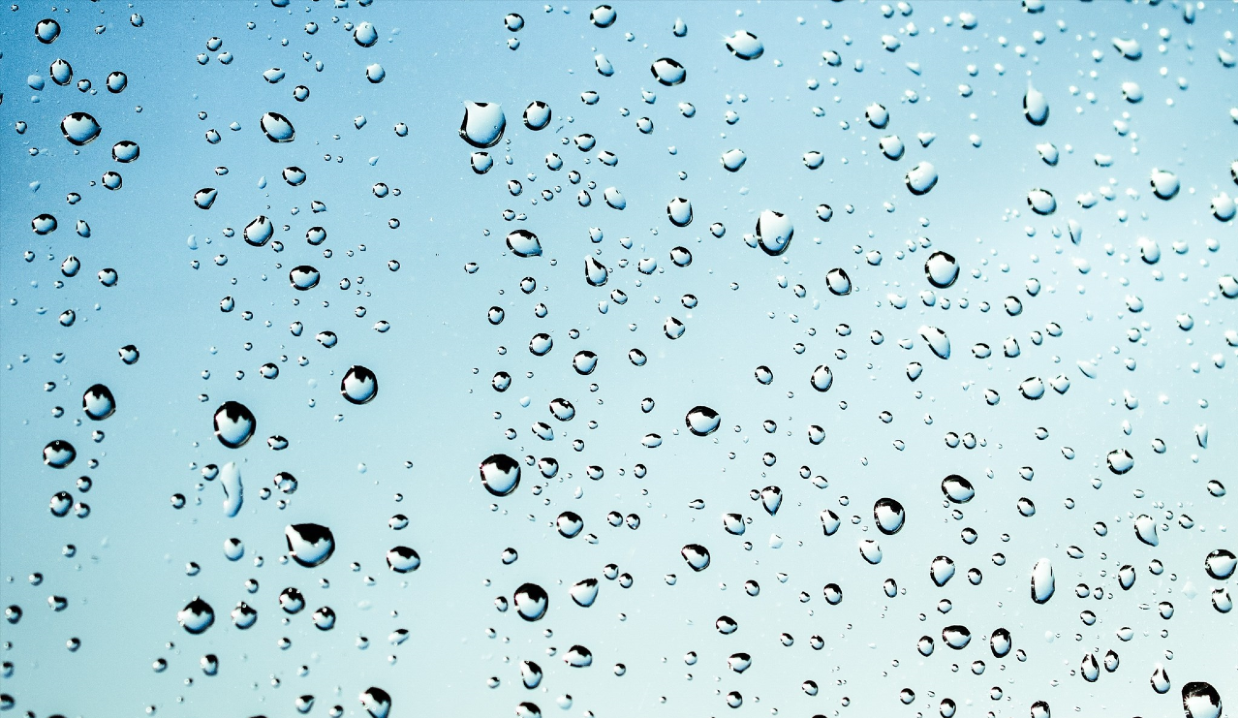
\includegraphics[width=\paperwidth]{Water3.png}};

\node[inner sep=0pt] (background) at (current page.center) {\includegraphics[width=\paperwidth]{WaterBackground1.png}};


\draw (current page.center)node [fill=blue!1!white!10,fill opacity=.3,text opacity=1,inner sep=2cm] { \Huge\centering\bfseries\sffamily\parbox[c][][t]{\paperwidth}{\centering \textcolor{Bittersweet}{WATR 081 - Fall 2020} \\\textcolor{BurntOrange}{Wastewater Treatment}\\[15pt] % Book title
% {\Large A Profound Subtitle}\\[20pt] % Subtitle
{\large Shabbir Basrai}}}; % Author name
\end{tikzpicture}
\begin{center}

\includegraphics[scale=0.5]{SCC_Logo_Primary.png}
\end{center}
\vfill
\endgroup

%----------------------------------------------------------------------------------------
%	COPYRIGHT PAGE
%----------------------------------------------------------------------------------------

\newpage
~\vfill
\thispagestyle{empty}

\noindent Copyright \copyright\ 2020 Shabbir Basrai\\ % Copyright notice
%
%\noindent \textsc{Published by Publisher}\\ % Publisher
%
%\noindent \textsc{book-website.com}\\ % URL
%
%\noindent Licensed under the Creative Commons Attribution-NonCommercial 3.0 Unported License (the ``License''). You may not use this file except in compliance with the License. You may obtain a copy of the License at \url{http://creativecommons.org/licenses/by-nc/3.0}. Unless required by applicable law or agreed to in writing, software distributed under the License is distributed on an \textsc{``as is'' basis, without warranties or conditions of any kind}, either express or implied. See the License for the specific language governing permissions and limitations under the License.\\ % License information, replace this with your own license (if any)

\noindent \textit{Revision Date: August, 2020} % Printing/edition date

%----------------------------------------------------------------------------------------
%	TABLE OF CONTENTS
%----------------------------------------------------------------------------------------

%\usechapterimagefalse % If you don't want to include a chapter image, use this to toggle images off - it can be enabled later with \usechapterimagetrue

\chapterimage{WastewaterTreatmentPlantAerialBandW.jpg} % Table of contents heading image

\pagestyle{empty} % Disable headers and footers for the following pages

\tableofcontents % Print the table of contents itself

\cleardoublepage % Forces the first chapter to start on an odd page so it's on the right side of the book

\pagestyle{fancy} % Enable headers and footers again

%----------------------------------------------------------------------------------------
%	PART
%----------------------------------------------------------------------------------------

\part{Week 1}

%----------------------------------------------------------------------------------------
%	CHAPTER 1
%----------------------------------------------------------------------------------------

% \chapterimage{chapter_head_2.pdf} % Chapter heading image

% \chapter{Text Chapter}

% \section{Paragraphs of Text}\index{Paragraphs of Text}


\chapterimage{Water1.png} % Chapter heading image

\chapter{Introduction to Wastewater Treatment}

% \section{Paragraphs of Text}\index{Paragraphs of Text}


% \everymath{\displaystyle}
% \linespread{2}%controls the spacing between lines. Bigger fractions means crowded lines%
% %\pagestyle{fancy}
% %\usepackage[margin=1 in, top=1in, includefoot]{geometry}
% %\everymath{\displaystyle}
% \linespread{2}%controls the spacing between lines. Bigger fractions means crowded lines%
% %\pagestyle{fancy}
% \pagestyle{fancy}
% \setlength{\headheight}{56.2pt}
% \colorlet{Mycolor1}{green!10!orange!90!}

% \chead{\ifthenelse{\value{page}=1}{
\includegraphics[scale=0.3]{SCC}\\ \textbf \textbf Introduction to Wastewater Treatment}}
% \rhead{\ifthenelse{\value{page}=1}{}{}}
% \lhead{\ifthenelse{\value{page}=1}{}{\textbf Introduction to Wastewater Treatment}}
% \rfoot{\ifthenelse{\value{page}=1}{Module 1: WATR 048 - Spring 2019}{Module 1: WATR 048 - Spring 2019}}

% \cfoot{Page \thepage\ of \pageref{LastPage}}
% \lfoot{Shabbir Basrai}
% \renewcommand{\headrulewidth}{2pt}
% \renewcommand{\footrulewidth}{1pt}

% \newcommand{\stkout}[1]{\ifmmode\text{\sout{\ensuremath{#1}}}\else\sout{#1}\fi}
% %Defining colour with different models.
% \definecolor{mypink1}{rgb}{0.858, 0.188, 0.478}
% \definecolor{mypink2}{RGB}{219, 48, 122}
% \definecolor{mypink3}{cmyk}{0, 0.7808, 0.4429, 0.1412}
% \definecolor{mygray}{gray}{0.6}
% \colorlet{LightRubineRed}{RubineRed!70!}
% \colorlet{Mycolor1}{green!10!orange!90!}
% \definecolor{Mycolor2}{HTML}{00F9DE}

% %New command used in the table with all available colour names
% \newcommand{\thiscolor}[1]{\texttt{#1} \hfill \fcolorbox{black}{#1}{\hspace{2mm}}}

% %This changes the row separation in the table
% \renewcommand{\arraystretch}{1.5}




%\noindent\textsc{Area \& Volume Math Problems}
%\definecolor{shadecolor}{RGB}{200,200,240}
% \item \noindent\textsc{Why Treat Wastewater}
\section{Why Treat Wastewater}\index{Why Treat Wastewater}
\begin{itemize}
\item Wastewater is used water from home and industries\\
\item Wastewater must be treated prior to returning it back into the environment - typically into the receiving waters which include lakes, rivers and ocean.


\item Wastewater treatment removes:
\begin{itemize}
\item organic matter
\item inorganic  pollutants including plant nutrients - nitrogen and phosphorous\\
\item pathogenic (disease causing) organisms\\
\end{itemize}

\item Wastewater treatment protects:
\begin{itemize}
\item The environment
\item Human health
\end{itemize}

\item In the receiving waters, inadequately treated wastewater discharge depletes dissolved oxygen levels - \hl{Eutrophication}, potentially destructing its normal aquatic life including fish.  Wastewater discharge promotes eutrophication due to:

\begin{itemize}
\item Nutrients such as nitrogen and phosphorous present in wastewater effluent promotes growth of plant and algal matter.  Dissolved oxygen is consumed as a part of the normal decay of this plant and algal matter.  
\item The consumption of organic material present in wastewater discharge by aerobic bacteria also results in oxygen depletion in the receiving waters.  


\end{itemize}
\end{itemize}

\section{Wastewater Treatment Regulations}\index{Wastewater Treatment Regulations}
% \begin{snugshade*}
% \item \noindent\textsc{Wastewater Treatment Regulations}
% \end{snugshade*}

\begin{itemize}
\item The \hl{National Pollutant Discharge Elimination System (NPDES) permit program} was created in 1972 by the Clean Water Act (CWA)
\item Applies to sources that discharge pollutants to waters of the United States.
\item Requires all facilities discharging “pollutants” into any body of water in the USA to obtain and comply with a \hl{NPDES permit}
\item NPDES permit \hl{establishes} \textul{discharge limits}, \textul{monitoring} and \textul{reporting} \hl{requirements}\\
\item The NPDES permitting and enforcement responsibilities have been delegated by the EPA to the State of California for implementation through the \hl{State Water Resources Control Board(SWRCB)} and the \textul{nine} \hl{Regional Water Quality Control Boards (Regional Water Boards)}.
\item In California, NPDES permits are also referred to as waste discharge requirements (WDRs) that regulate discharges to waters of the United States.
\end{itemize}


\section{Wastewater Process Overview}\index{Wastewater Process Overview}
Wastewater treatment involves the following elements:

\subsection{Generation}\index{Generation}

Wastewater originates from domestic, industrial, commercial or agricultural activities. The characteristics of wastewater vary depending on the source. Types of wastewater include: 
\begin{itemize}
\item \hl{Domestic Sewage:}  wastewater derived principally from dwellings, business buildings, institutions, and \\
\item \hl{Industrial Sewage:}  liquid waste from industrial processes\\
\end{itemize}
Typical per person generation of wastewater in the USA is about 70-100 gallons per day

\subsection{Collections}\index{Collections}

\begin{itemize}
\item Wastewater is collected from its point of origin - home, businesses, industries etc. and conveyed via sewer lines to a centralized wastewater treatment facility.  
\item When the rainwater drainage is made part of the sewer system, the system is termed as \hl{Combined System}.  
\item The system where the sewage is conveyed separately from the stormwater flows is termed as \hl{Separated System}.  
\item In the Separated System, the Sanitary Sewers convey the wastewater and the Stormwater Sewer conveys the storm water flows.  
\item For the Combined System, rainstorms pose the threat of overwhelming the sewers and the treatment plant
\end{itemize}  
\begin{center}
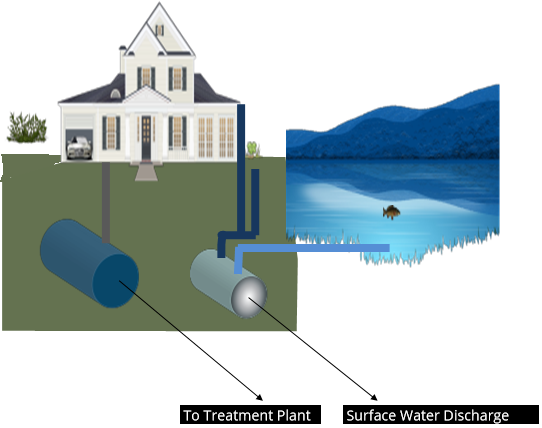
\includegraphics[scale=0.45]{SeperatedSystem1} \hspace{1 cm} 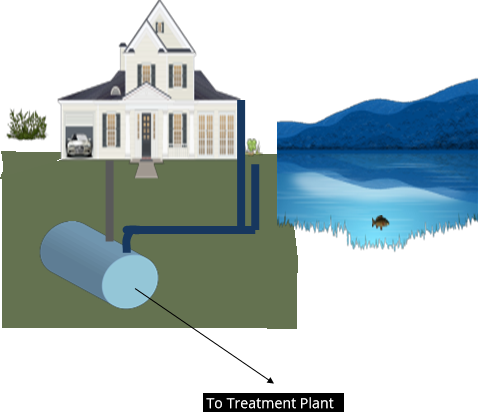
\includegraphics[scale=0.45]{CombinedSystem1}
\end{center}
			\hspace{2.6cm} Separated System \hspace{3.2cm} \parbox{\textwidth}{Combined System}\\

\subsection{Treatment}\index{Treatment}

\begin{itemize}
\item Wastewater treatment can involve physical, chemical or biological processes or combinations of these processes depending on the required outflow standards. 
\item Wastewater treatment typically involves a series of steps with increasing level of treatment:
\begin{itemize}
\item \hl{Preliminary}:  The preliminary process removes large/coarse solids which include rocks, tree branches, grit and other debris present in wastewater.
\item \hl{Primary}:  The primary process is also a physical process where the separable wastewater solids - solids that float and solids that can settle, are removed.  
\item \hl{Secondary}:  Secondary treatment is a biological treatment process where microorganisms consume the organic matter present in the wastewater. 
\item \hl{Tertiary or Advanced Treatment}:  The tertiary/advanced treatment processes improve the quality of treated water beyond the secondary treatment level.  This process may include nutrient removal and disinfection.

\item Solids treatment processes are primarily geared to ensure that the solids generated as part of the wastewater treatment processes, meet the federal regulatory requirements established for wastewater generated solids, at the lowest cost and environmental impact.
\end{itemize}

A generalized layout/process sequencing in a wastewater treatment plant is shown below:
\begin{center}
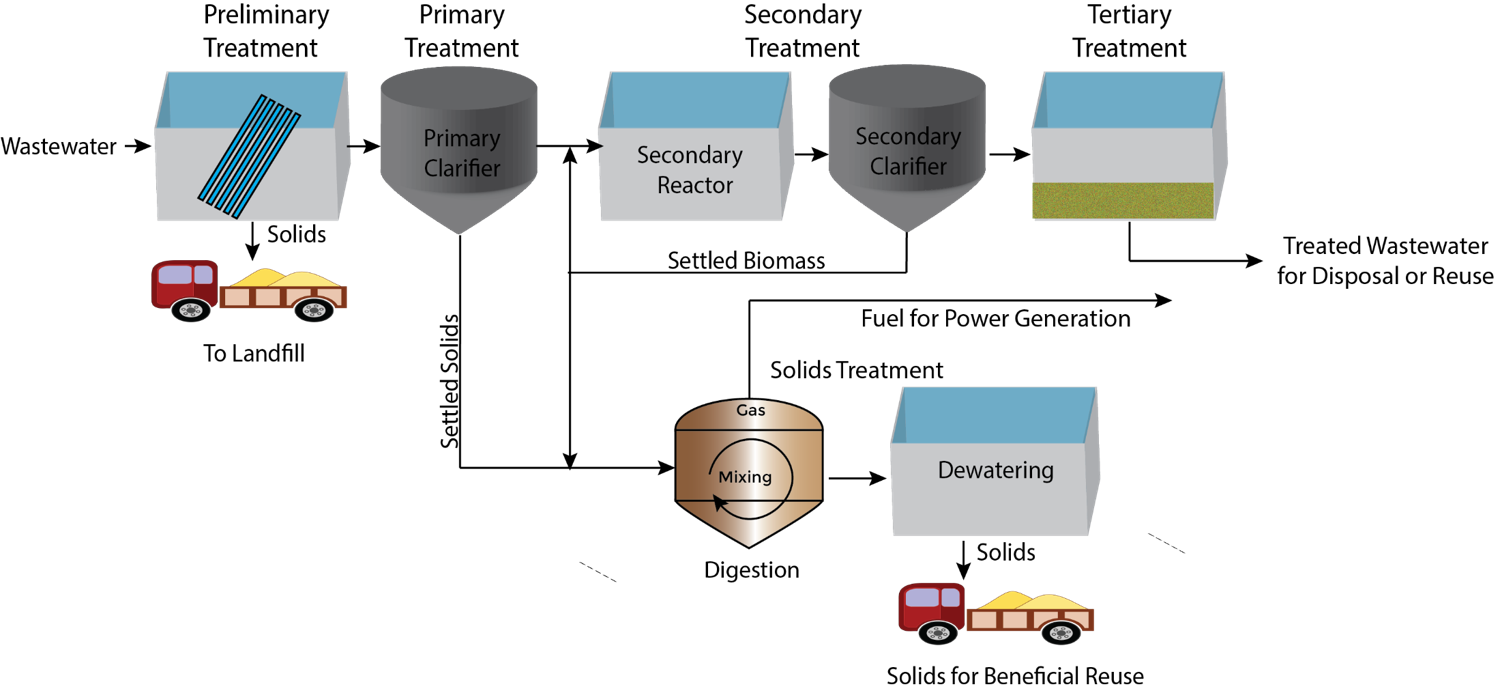
\includegraphics[scale=0.6]{TreatmentFlow}
\end{center}
Individual wastewater treatment processes involve different process options or sequences which are illustrated in the graphic below:
\begin{center}
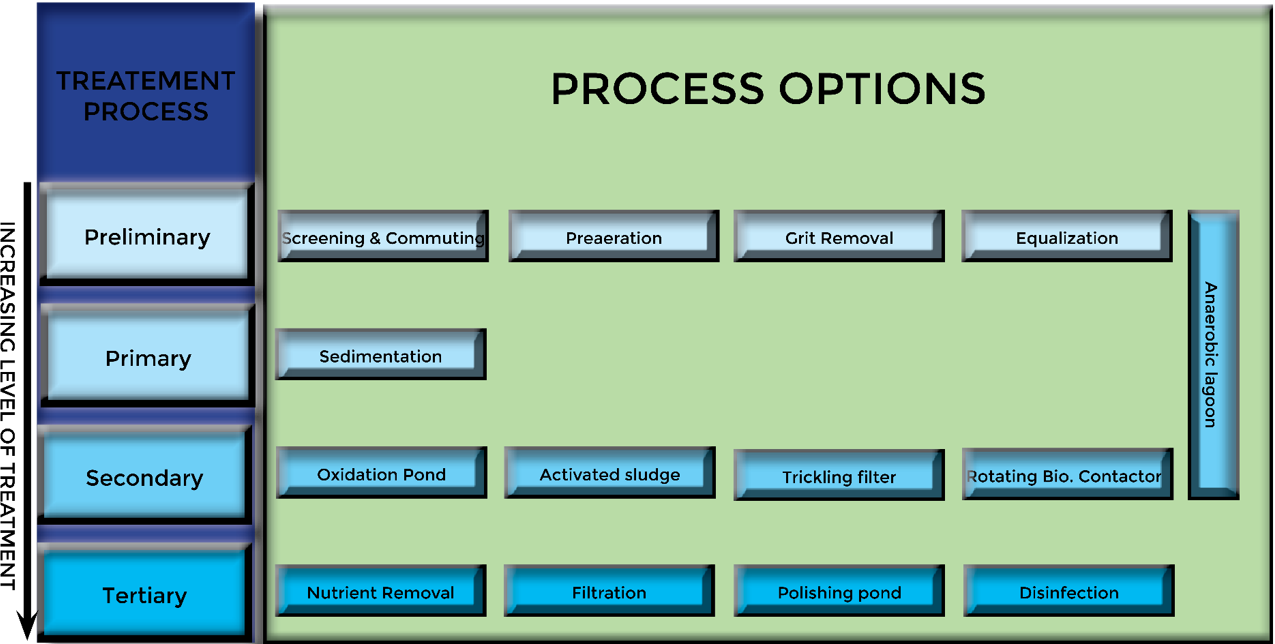
\includegraphics[scale=0.42]{Treatment}
\end{center}
\end{itemize}
As the treatment process becomes more advanced along with the increasing awareness of the resources involved in the treatment, there is a move underway to transform Wastewater Treatment Plants (WWTF) to Renewable Resource Recovery Facilities (RRRF) or Water Resource Recovery Facilities (WRRF) - one which produces clean water, recovers energy and generates nutrients.

\subsection{Disposal or Reuse}\index{Disposal or Reuse}

\begin{itemize}
\item Wastewater treatment processes can be designed to \hl{dispose} the treated water where the water is reintroduced to the environment or for \hl{reuse} where the treated water is \hl{reclaimed} or \hl{recycled} - for various purposes including irrigation, industrial use or for potable use.
\item Water disposal methods include:\\
\begin{itemize}
\item \hl{Surface water discharge}
\item \hl{Subsurface discharge}
\end{itemize}
\item Water reuse methods include:\\
\begin{itemize}
\item Potable water reuse
\begin{itemize}
\item \hl{Indirect potable reuse:}  Here the treated water is blended with groundwater or surface water and then reclaimed and treated further 
for drinking (potable) water use
\item \hl{Direct potable reuse:}  Here the treated wastewater is subjected to advanced treatment and introduced directly into a municipal water supply system
\end{itemize}
\item Water reclamation for irrigation or industrial use\\
\item Land application for beneficial use\\
\end{itemize}
\item Solids generated from the wastewater treatment process may be removed and disposed to a landfill or subject to further treatment which may allow for energy recovery - from the organic solids and for beneficial reuse due to its plant nutrient content.\\
\end{itemize}


\chapterimage{MathCover.png} % Chapter heading image
\chapter{Wastewater Math}


% \begin{enumerate}
% \definecolor{shadecolor}{RGB}{200, 200, 240}
% \begin{snugshade*}
%\section{Units and Unit Conversion}\index{Units and Unit Conversion}
% 	\item \noindent\textsc{Units and Unit Conversion}
% \end{snugshade*}
\section{Unit Conversions}\index{Unit Conversions}
For converting one measurement unit to another.

Step 1:  \texthl{Make sure the original unit is for the same measurement as the converted (desired) unit.}  So if the original unit is for area, say in ft$^2$ the converted unit should be another area unit such as in$^2$ or acre but it cannot be gallons as gallon is a unit of volume.

Step 2: Write down the conversion formula as:

$Quantity \enspace in \enspace converted \enspace unit = Quantity \enspace (\cancel{Original \enspace Unit}) *   Conversion  \enspace Factor \enspace  \dfrac{Conversion \enspace unit}{\cancel{Original \enspace unit}}$


\begin{table}[h!]

\begin{center}
    \begin{tabular}{ | p{4cm} |p{8cm}|}
    \hline
    
    
Length  & inches, ft, miles\\
\hline 
Area  & ft$^2$, acres \\
\hline 
Volume & ft$^3$, gallons, acres-ft.\\
\hline 
Density & weight per volume, lbs/ft$^3$, lbs/gallon\\
\hline 
Flow & ft$^3$/min, MGD, acres-ft/day\\
\hline 

	

    \end{tabular}
 \caption{Common units in wastewater calculations}	
    \end{center}

    \end{table}



\section{Example Problems}
Problem 1\\
Convert 1000 $ft^3$ to cu. yards\\

$1000 \cancel{ft^3}*\dfrac{cu.yards}{27\cancel{ft^3}} = 37 cu.yards$

Problem 2\\
Convert 10 gallons/min to $ft^3$/hr\\

$\dfrac{10 \cancel{gallons}}{\cancel{min}}*  \dfrac{ft^3}{7.48 \cancel{gallons}}  * \dfrac{60 \cancel{min}}{hr}   = \dfrac{80.2ft^3}{hr}$


Problem 3\\
Convert 100,000 $ft^3$ to acre-ft.\\
$100,000 \cancel{ft^3} * \dfrac{acre-ft}{43,560 \cancel{ft^2-ft}} =  2.3 acre-ft$\\
\textbf{Note:} From the conversion table: acre = 43,560 $ft^2$\\
Thus, acre-ft  = 43,560 $ft^2$-ft\\

\section{Pounds Formula}\index{Pounds Formula}
%\section{Pounds Formula}\index{Pounds Formula}

% \begin{snugshade*}
% \item \noindent\textsc{Pounds Formula}
% \end{snugshade*}
Pounds formula is used for:
\begin{itemize}
\item Calculating the quantity in pounds of a particular wastewater constituent entering or leaving a wastewater treatment process
\item Calculating the pounds of chemicals to be added\\
\end{itemize}
So if the concentration of a particular constituent (in mg/liter) and the volume or flow of wastewater is given, one can calculate the amount of that constituent in pounds using the following – Pounds Formula:
$$lbs \enspace \textbf{or} \enspace \dfrac{lbs}{day}=Concentration\Big(\frac{mg}{l}\Big)*8.34*volume(MG) \enspace \textbf{or} \enspace Flow (MGD)$$\\

The Davidson Pie as shown below provides a pictorial representation of the Pounds Formula.

	\begin{figure}[H]
\begin{center}
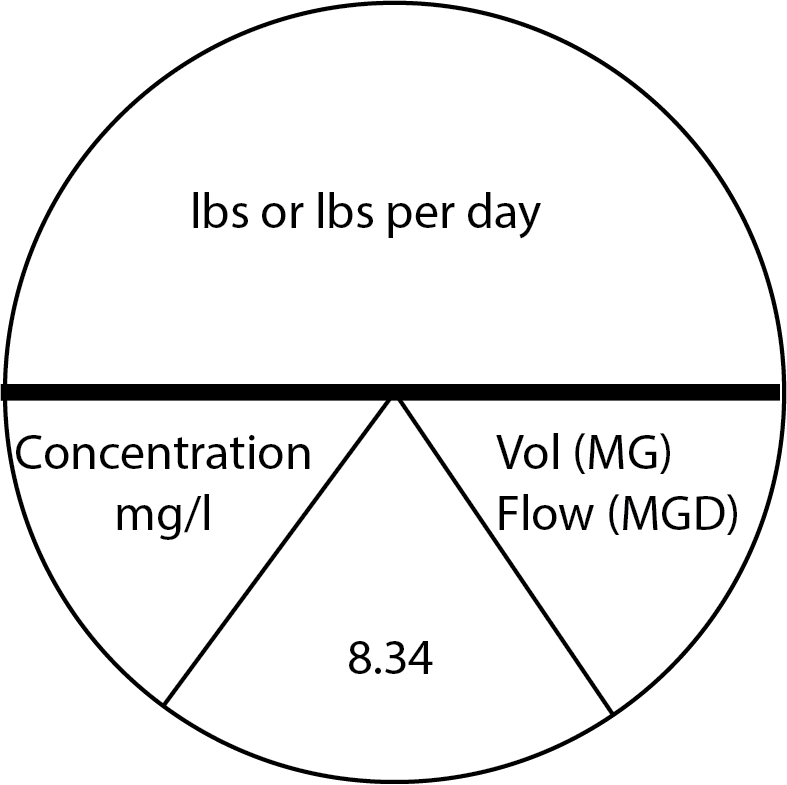
\includegraphics[scale=0.5]{PoundsFormula}
\end{center}
\caption{Davidson Pie}
\end{figure}

In the Pounds Formula, there are three variables – lbs, concentration and volume, and one constant - 8.34.  Knowing any of the two variables in the formula, one can calculate the third (unknown) variable by rearranging the equation.\\

\vspace{0.3cm}
Davidson Pie provides a pictorial reference for calculating any unknown variable.  If for example, if Concentration is unknown, it can be calculated as follows: \\$$Concentration\Big(\frac{mg}{l}\Big)=\dfrac{lbs \enspace \textbf{or} \enspace \dfrac{lbs}{day}}{8.34*Volume(MG) \enspace \textbf{or} \enspace Flow (MGD)}$$\\

\vspace{0.3cm}

Likewise, if Volume (or Flow) is the unknown variable. it can be calculated as:  \\$$Volume (MG) \enspace or \enspace Flow(MGD)=\dfrac{lbs \enspace \textbf{or} \enspace \dfrac{lbs}{day}}{Concentration\Big(\dfrac{mg}{l}\Big)* \enspace 8.34  }$$
\newpage
\section{Concentration}\index{Concentration}

Concentration is typically expressed as mg/l which is the weight of the constituent (mg) in 1 l (liter) of solution (wastewater).  As 1 l of water weighs 1 million mg, a concentration of 1 mg/l implies 1 mg of constituent per 1 million mg of water or one part per million (ppm).   \textbf{Thus, mg/l and ppm are synonymous.}\\  
Sometimes the constituent concentration is expressed in terms of percentage.\\
\vspace{6pt}
For example:  sludge containing 5\% solids or a 12.5\% chlorine concentration solution.\\
\vspace{6pt}
As one liter of water weighs 1,000,000 mg, one percent of that weight is 10,000 mg.  So 1\% solids implies 10,000 mg of solids per liter or 10,000 mg/l or 10,000 ppm.\\
\vspace{6pt}
$1\% \enspace concentration = 10,000 \enspace ppm \enspace or \enspace\dfrac{mg}{l}$\\
$0.1\% \enspace concentration = 1,000 \enspace ppm \enspace or \enspace \dfrac{mg}{l}$\\
$0.01\% \enspace concentration = 100 \enspace ppm \enspace or \enspace \dfrac{mg}{l}$\\
$10\% \enspace concentration = 100,000 \enspace ppm \enspace or \enspace \dfrac{mg}{l}$\\
$5\% \enspace concentration = 50,000 \enspace ppm \enspace or \enspace \dfrac{mg}{l}$\\
$12.5\% \enspace concentration = 125,000 \enspace ppm \enspace or \enspace \dfrac{mg}{l}$\\

\subsection{Example Problems}
% \hl{Example Problems}\\

Problem 1\\Calculate the lbs/day of solids entering the plant given the influent flow is 5 MGD with an average solids concentration  of 250 mg/l.\\

Solution\\

Applying lbs formula:\\
$\dfrac{lbs}{day}=5 MGD *250\dfrac{mg}{l}*8.34 = \boxed{10,425\dfrac{lbs}{day}}$
\\
\vspace{6pt}
Problem 2\\Calculate the lbs of solids in the primary sludge if the sludge flow is 7500 gallons and the solids concentration is 4.5\%.\\
Solution\\
Applying lbs formula:\\
$lbs \enspace solids = \dfrac{7500}{1,000,000}MG * 4.5*10,000 *8.34 = \boxed{2,815 \enspace lbs \enspace solids}$\\
\textbf{Note:}\\  
1) 7500 gallons was converted to MG by dividing by 1,000,000\\
$7500 \enspace gallons * \dfrac{1 MG}{1,000,000 \enspace gallon}$\\
2) 4.5\% was converted to mg/l by multiplying by 10,000 as 1\%=10,000mg/l


\section{Area \& Volume}\index{Area \& Volume}
% \section{Area \& Volume}\index{Area \& Volume}

% \begin{snugshade*}
% 	\item \noindent\textsc{Area \& Volume}
% \end{snugshade*}

\begin{center}
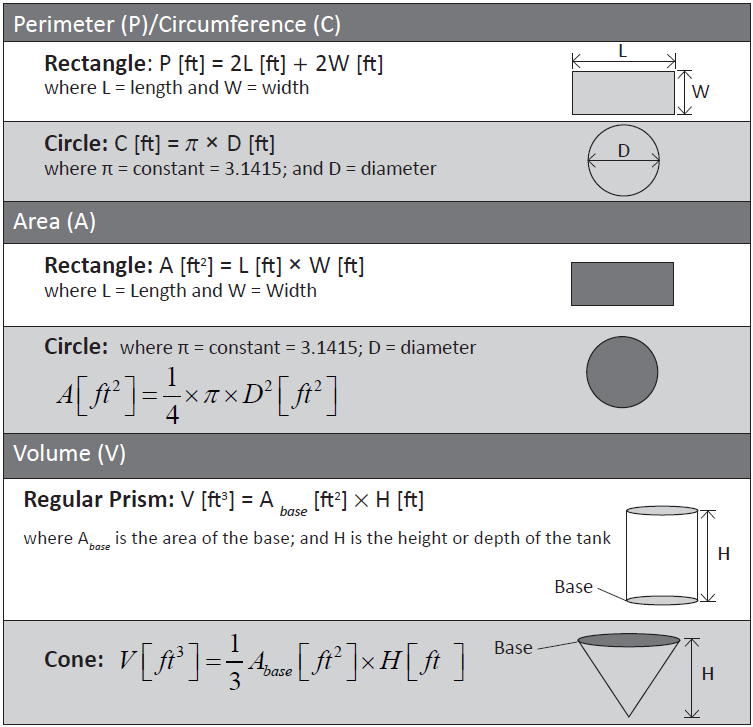
\includegraphics[scale=0.5]{Area&VolumeFormula}
\end{center}
\subsection{Example Problems}
% \hl{Example Problems}\\
\begin{enumerate}

\item The floor of a rectangular building is 20 feet long by 12 feet wide and the inside walls are 10 feet high. Find the total surface area of the inside walls of this building\\
Solution:\\
% \begin{center}
\begin{tikzpicture}
	%%% Edit the following coordinate to change the shape of your
	%%% cuboid
      
	%% Vanishing points for perspective handling
	\coordinate (P1) at (-7cm,1.5cm); % left vanishing point (To pick)
	\coordinate (P2) at (8cm,1.5cm); % right vanishing point (To pick)

	%% (A1) and (A2) defines the 2 central points of the cuboid
	\coordinate (A1) at (0em,0cm); % central top point (To pick)
	\coordinate (A2) at (0em,-2cm); % central bottom point (To pick)

	%% (A3) to (A8) are computed given a unique parameter (or 2) .8
	% You can vary .8 from 0 to 1 to change perspective on left side
	\coordinate (A3) at ($(P1)!.8!(A2)$); % To pick for perspective 
	\coordinate (A4) at ($(P1)!.8!(A1)$);

	% You can vary .8 from 0 to 1 to change perspective on right side
	\coordinate (A7) at ($(P2)!.7!(A2)$);
	\coordinate (A8) at ($(P2)!.7!(A1)$);

	%% Automatically compute the last 2 points with intersections
	\coordinate (A5) at
	  (intersection cs: first line={(A8) -- (P1)},
			    second line={(A4) -- (P2)});
	\coordinate (A6) at
	  (intersection cs: first line={(A7) -- (P1)}, 
			    second line={(A3) -- (P2)});

	%%% Depending of what you want to display, you can comment/edit
	%%% the following lines

	%% Possibly draw back faces

	\fill[gray!40] (A2) -- (A3) -- (A6) -- (A7) -- cycle; % face 6
	\node at (barycentric cs:A2=1,A3=1,A6=1,A7=1) {\tiny Floor=W*L};
	
	\fill[gray!50] (A3) -- (A4) -- (A5) -- (A6) -- cycle; % face 3
	\node at (barycentric cs:A3=1,A4=1,A5=1,A6=1) {\tiny Wall - W*H};
	
	\fill[gray!10, opacity=0.2] (A5) -- (A6) -- (A7) -- (A8) -- cycle; % face 4
	\node at (barycentric cs:A5=1,A6=1,A7=1,A8=1) {\tiny Wall - L*H};
	
	\fill[gray!10,opacity=0.5] (A1) -- (A2) -- (A3) -- (A4) -- cycle; % f2
	\node at (barycentric cs:A1=1,A2=1,A3=1,A4=1) {\tiny Wall - L*H};
	
	\fill[gray!40,opacity=0.2] (A1) -- (A4) -- (A5) -- (A8) -- cycle; % f5
	\node at (barycentric cs:A1=1,A4=1,A5=1,A8=1) {\tiny Ceiling=W*L};	
	
	\draw[thick,dashed] (A5) -- (A6);
	\draw[thick,dashed] (A3) -- (A6);
	\draw[thick,dashed] (A7) -- (A6);

	%% Possibly draw front faces

	%\fill[orange] (A1) -- (A8) -- (A7) -- (A2) -- cycle; % face 1
	\node at (barycentric cs:A1=1,A8=1,A7=1,A2=1) {\tiny Wall - W*H};
	


	%% Possibly draw front lines
	\draw[thick] (A1) -- (A2);

	\draw[<->] (-1.8,0.38) -- (-1.8,-1.3)node [midway, above=-1.8mm] {\hspace{-1.3cm}\tiny Height=10'};
	\draw[<->] (-1.6,-1.4) -- (-.3,-2.1)node [midway, above=-2.6mm] {\hspace{-1.3cm}\tiny Length=20'};
	\draw[<->] (2.6,-1.13) -- (0.2,-2.2)node [midway, below=.6mm] {\hspace{1.2cm}\tiny Width=12'};
	\draw[thick] (A3) -- (A4);
	\draw[thick] (A7) -- (A8);
	\draw[thick] (A1) -- (A4);
	\draw[thick] (A1) -- (A8);
	\draw[thick] (A2) -- (A3);
	\draw[thick] (A2) -- (A7);
	\draw[thick] (A4) -- (A5);
	\draw[thick] (A8) -- (A5);
	
	% Possibly draw points
	% (it can help you understand the cuboid structure)
%	\foreach \i in {1,2,...,8}
%	{
%	  \draw[fill=black] (A\i) circle (0.15em)
%	    node[above right] {\tiny \i};
%	}
	% \draw[fill=black] (P1) circle (0.1em) node[below] {\tiny p1};
	% \draw[fill=black] (P2) circle (0.1em) node[below] {\tiny p2};
\end{tikzpicture}\\
% \end{center}
2 Walls W*H + 2 Walls L*H= $2*12*10ft^2 + 2*20*10ft^2$\\
$=240+400=\boxed{640ft^2}$\\

2 Walls W*H + 2 Walls L*H + Floor + Ceiling= $2*12*10ft^2 + 2*20*10ft^2 + 2*12*20ft^2$\\
$=240+400+480=\boxed{1,120ft^2}$\\

\item How many gallons of paint will be required to paint the inside walls of a 40 ft long x 65 ft wide x 20 ft high tank if the paint coverage is 150 sq. ft per gallon.  Note:  We are painting walls only.  Disregard the floor and roof areas.\\
Solution:\\
\vspace{0.3cm}
% \begin{center}
\begin{tikzpicture}
	%%% Edit the following coordinate to change the shape of your
	%%% cuboid
      
	%% Vanishing points for perspective handling
	\coordinate (P1) at (-7cm,1.5cm); % left vanishing point (To pick)
	\coordinate (P2) at (8cm,1.5cm); % right vanishing point (To pick)

	%% (A1) and (A2) defines the 2 central points of the cuboid
	\coordinate (A1) at (0em,0cm); % central top point (To pick)
	\coordinate (A2) at (0em,-2cm); % central bottom point (To pick)

	%% (A3) to (A8) are computed given a unique parameter (or 2) .8
	% You can vary .8 from 0 to 1 to change perspective on left side
	\coordinate (A3) at ($(P1)!.8!(A2)$); % To pick for perspective 
	\coordinate (A4) at ($(P1)!.8!(A1)$);

	% You can vary .8 from 0 to 1 to change perspective on right side
	\coordinate (A7) at ($(P2)!.7!(A2)$);
	\coordinate (A8) at ($(P2)!.7!(A1)$);

	%% Automatically compute the last 2 points with intersections
	\coordinate (A5) at
	  (intersection cs: first line={(A8) -- (P1)},
			    second line={(A4) -- (P2)});
	\coordinate (A6) at
	  (intersection cs: first line={(A7) -- (P1)}, 
			    second line={(A3) -- (P2)});

	%%% Depending of what you want to display, you can comment/edit
	%%% the following lines

	%% Possibly draw back faces

	\fill[gray!40] (A2) -- (A3) -- (A6) -- (A7) -- cycle; % face 6
	\node at (barycentric cs:A2=1,A3=1,A6=1,A7=1) {};
	
	\fill[gray!50] (A3) -- (A4) -- (A5) -- (A6) -- cycle; % face 3
	\node at (barycentric cs:A3=1,A4=1,A5=1,A6=1) {\tiny Wall - W*H};
	
	\fill[gray!10, opacity=0.2] (A5) -- (A6) -- (A7) -- (A8) -- cycle; % face 4
	\node at (barycentric cs:A5=1,A6=1,A7=1,A8=1) {\tiny Wall - L*H};
	
	\fill[gray!10,opacity=0.5] (A1) -- (A2) -- (A3) -- (A4) -- cycle; % f2
	\node at (barycentric cs:A1=1,A2=1,A3=1,A4=1) {\tiny Wall - L*H};
	
	\fill[gray!40,opacity=0.2] (A1) -- (A4) -- (A5) -- (A8) -- cycle; % f5
	\node at (barycentric cs:A1=1,A4=1,A5=1,A8=1) {};	
	
	\draw[thick,dashed] (A5) -- (A6);
	\draw[thick,dashed] (A3) -- (A6);
	\draw[thick,dashed] (A7) -- (A6);

	%% Possibly draw front faces

	%\fill[orange] (A1) -- (A8) -- (A7) -- (A2) -- cycle; % face 1
	\node at (barycentric cs:A1=1,A8=1,A7=1,A2=1) {\tiny Wall - W*H};
	


	%% Possibly draw front lines
	\draw[thick] (A1) -- (A2);

	\draw[<->] (-1.8,0.38) -- (-1.8,-1.3)node [midway, above=-1.8mm] {\hspace{-1.3cm}\tiny Height=20'};
	\draw[<->] (-1.6,-1.4) -- (-.3,-2.1)node [midway, above=-2.6mm] {\hspace{-1.3cm}\tiny Length=40'};
	\draw[<->] (2.6,-1.13) -- (0.2,-2.2)node [midway, below=.6mm] {\hspace{1.2cm}\tiny Width=65'};
	\draw[thick] (A3) -- (A4);
	\draw[thick] (A7) -- (A8);
	\draw[thick] (A1) -- (A4);
	\draw[thick] (A1) -- (A8);
	\draw[thick] (A2) -- (A3);
	\draw[thick] (A2) -- (A7);
	\draw[thick] (A4) -- (A5);
	\draw[thick] (A8) -- (A5);
	
	% Possibly draw points
	% (it can help you understand the cuboid structure)
%	\foreach \i in {1,2,...,8}
%	{
%	  \draw[fill=black] (A\i) circle (0.15em)
%	    node[above right] {\tiny \i};
%	}
	% \draw[fill=black] (P1) circle (0.1em) node[below] {\tiny p1};
	% \draw[fill=black] (P2) circle (0.1em) node[below] {\tiny p2};
\end{tikzpicture}\\
% \end{center}
\vspace{0.3cm}
2 Walls W*H + 2 Walls L*H = $2*65*20ft^2 + 2*40*20ft^2= 2,600+1,600=4,200ft^2$\\
$\implies @150\dfrac{ft^2}{gal} \enspace paint \enspace coverage \enspace \rightarrow \enspace \dfrac{4,200\cancel{ft^2}}{150\dfrac{\cancel{ft^2}}{gal}}=\boxed{28 \enspace gallons}$
\vspace{0.3cm}
\item What is the circumference of a 100 ft diameter circular clarifier?\\
\vspace{0.3cm}
Solution:\\
\vspace{0.3cm}
$Circumference=\pi*D=3.14*100ft=\boxed{314ft}$
\vspace{0.3cm}
\item If the surface area of a clarifier is 5,025$ft^2$, what is its diameter?\\
\vspace{0.3cm}
Solution:\\
\vspace{0.3cm}
$Surface \enspace area=\dfrac{\pi}{4}*D^2 \enspace \implies 5025(ft^2)=0.785*D^2 (ft^2)$\\
$\implies D^2=\dfrac{5025}{0.785} \implies D=\sqrt{6401.3}=\boxed{80ft}$
\vspace{0.3cm}

\item How many gallons of wastewater would 600 feet of 6-inch diameter pipe hold, approximately?\\
\vspace{0.3cm}
Solution:\\

\vspace{0.3cm}
% \begin{center}
\begin{tikzpicture}
\draw (0,0) ellipse (0.1cm and 0.3cm);
\draw (10,0) ellipse (0.1cm and 0.3cm);
\draw [-] (0,-0.29) -- (10,-0.29);
\draw [-] (0,0.29) -- (10,0.29);
\draw [<->] (10,-0.28) -- (10,0.28) node [midway, below=-3mm] {\hspace{2.6cm}Diameter=6"};
\draw [<->] (0,-.68) -- (10,-.68)node [midway, below] {\hspace{0.9cm}Length=600'};
\end{tikzpicture}
% \end{center}
\vspace{0.3cm}
$Volume=\dfrac{\pi}{4}D^2*L=0.785*\Big(\dfrac{6}{12}\Big)^2*600\cancel{ft^3}*7.48\dfrac{gallons}{\cancel{ft^3}}=\boxed{881 \enspace gallons}$
\vspace{0.5cm}
\item A 110 ft diameter digester with a 12 ft deep cone is operated at a side water depth of 20 ft.  Caluclate the volume of sludge in the digester in $ft^3$ and gallons.\\
\vspace{0.3cm}
Solution:\\
\vspace{0.3cm}
% \begin{center}
\begin{tikzpicture}
\draw (0,0) ellipse (2cm and 0.3cm);
\draw (0,-2.3) ellipse (2cm and 0.3cm);
\draw (0,-.8) ellipse (2cm and 0.3cm);
\draw [-] (2,-2.3) -- (2,0);
\draw [<->] (-2,0) -- (2,0) node [midway, below=-0.9cm] {\hspace{0.9cm}Diameter (D)=110'}; 
\draw [<->] (-2.6,-2.3) -- (-2.6,0) node [midway, below=-.3cm] {\hspace{-2.6cm}Cylinder Height};
\draw [<->] (2.5,-2.3) -- (2.5,-0.8) node [midway, below=-0.2cm] {\hspace{5.2cm}Side Water Depth (SWD) =20'};
\draw [-] (0,-4) -- (2,-2.3);
\draw [-] (0,-4) -- (-2,-2.3);
\draw [-] (0,-4) -- (2,-2.3);
\draw [-] (-2,0) -- (-2,-2.3);
\draw [<->] (2.5,-2.3) -- (2.5,-4)node [midway, below=-0.4cm] {\hspace{3.8cm}Cone Depth (CD)=12'};
\end{tikzpicture}\\
% \end{center}
$Digester \enspace volume=Volume_{cylinder}+Volume_{cone}$\\
$\implies Digester \enspace volume=\dfrac{\pi}{4}D^2*SWD+\dfrac{1}{3}*\Bigg(\pi*D^2*CD\Bigg)$\\
\vspace{0.3cm}
$=0.785*110^2*20+1.05*110^2*12=\boxed{227,988ft^3}$\\
\vspace{0.3cm}
$227,988\cancel{ft^3}*7.48\dfrac{gallons}{\cancel{ft^3}}=\boxed{1,705,352 \enspace gallons}$
\end{enumerate}

\section{Process Removal Efficiency}\index{Process Removal Efficiency}

% \section{Process Removal Efficiency}\index{Process Removal Efficiency}
% \begin{snugshade*}
% 	\item \noindent\textsc{Process Removal Efficiency}
% \end{snugshade*}
\begin{itemize}
\item Process removal rate or removal efficiency is the percentage of the inlet concentration removed.  
\item It is used for quantifying the pollutant removal during wastewater treatment and is established based upon the amount of a particular wastewater constituent entering and leaving a treatment process.

\item $Process \enspace Removal \enspace Rate \enspace (\%) = \dfrac{Pollutant \enspace  In-Pollutant\enspace  Out}{Pollutant \enspace In}*100$\\

\item If 10 units of a pollutant are entering a process and 8 units of pollutant are leaving (process removes 2 units), then the process removal rate for that pollutant is (10-8)/10*100=20\%.  In this example the process is 20\% efficient in removing that particular pollutant.

\item The amount of pollutant can be measured in terms of concentration (mg/l) or in terms of mass loading (lbs).  The pounds formula is used for calculating the mass loadings.  
\end{itemize}
The above example is for calculating the removal efficiency using the inlet and outlet concentrations or mass loading.\\
The methods below can be used for calculating either the inlet or outlet pollutant concentrations, if the removal efficiency and the corresponding inlet or outlet concentrations are given. 


\hl{Case 1:  Calculating outlet conc. (X) given the inlet conc. and removal efficiency (RE\%):}

\tikzstyle{block} = [rectangle, draw, fill=red!40, 
    text width=6em, text centered, rounded corners, minimum height=3em]
\tikzstyle{arrow} = [draw, -latex']
\begin{figure}[!h]
\centering
\begin{tikzpicture}[node distance =1.5cm, auto]
    \draw ++(0,0) node [block] (Process) {Process};
   \node[node distance=1.9in] (dummy_in) [left of=Process] {In};
   \node[node distance=1.9in] (dummy_out) [right of=Process] {Out};
	\node (Removal) [below of=Process, yshift=-0in] {${Removal \enspace Efficiency=RE\% \enspace (Given)}$};
    \path [arrow] (dummy_in)-- (Process)  node [above] {\hspace{-5.8cm}$A \enspace mg/l \enspace (Given) $} node [below] {\hspace{-5.8cm}$100 \enspace mg/l$};
    \path [arrow] (Process) -- (dummy_out)  node [above] {\hspace{-4cm}$X \enspace mg/l \enspace (Unknown)$} node [below] {\hspace{-3.9cm}($100-RE\%)\enspace mg/l$};
   \draw[arrow] (Process) -- (Removal);
\end{tikzpicture}
\end{figure}
Using the fact that if the inlet concentration was 100 mg/l, the outlet concentration would be 100 minus the removal efficiency.\\
Setup the equation as:  $\dfrac{Out}{In}: \enspace \dfrac{X \enspace mg/l}{A \enspace mg/l}=\dfrac{100-RE\%}{100}$\\
Calculate X using cross multiplication - if $\dfrac{A}{B}=\dfrac{C}{D} \implies A=B*\dfrac{C}{D}$:\\
$X \enspace mg/l=A \enspace mg/l*\dfrac{100-RE\%}{100}$\\


\hl{Case 2:  Calculating inlet conc. (X) given the outlet conc. and removal efficiency (RE\%):}

\begin{figure}[!h]
\centering
\begin{tikzpicture}[node distance =1.5cm, auto]
    \draw ++(0,0) node [block] (Process) {Process};
   \node[node distance=1.9in] (dummy_in) [left of=Process] {In};
   \node[node distance=1.9in] (dummy_out) [right of=Process] {Out};
	\node (Removal) [below of=Process, yshift=-0in] {$Removal \enspace Efficiency=RE\% \enspace (Given)$};
    \path [arrow] (dummy_in)-- (Process)  node [above] {\hspace{-5.8cm}$X \enspace mg/l \enspace (Unknown)$} node [below] {\hspace{-5.8cm}$100 \enspace mg/l$};
    \path [arrow] (Process) -- (dummy_out)  node [above] {\hspace{-4cm}$A \enspace mg/l \enspace (Given)$} node [below] {\hspace{-3.9cm}($100-RE\%)\enspace mg/l$};
   \draw[arrow] (Process) -- (Removal);
\end{tikzpicture}
\end{figure}
Using the fact that if the inlet concentration was 100 mg/l, the outlet concentration would be 100 minus the removal efficiency.\\
Setup the equation as:  $\dfrac{In}{Out}: \enspace \dfrac{X \enspace mg/l}{A \enspace mg/l}=\dfrac{100}{100-RE\%}$\\
\vspace{0.3cm}
Calculate X using cross multiplication - if $\dfrac{A}{B}=\dfrac{C}{D} \implies A=B*\dfrac{C}{D}$:\\
$X \enspace mg/l=A \enspace mg/l*\dfrac{100}{100-RE\%}$\\

\vspace{0.4cm}
\subsection{Example Problems}
% \hl{Example Problems:}\\

\begin{enumerate}

\item What is the \% removal efficiency if the influent concentration is 10 mg/L and the effluent concentration is 2.5 mg/L?\\
$Removal \enspace Rate (\%) = \dfrac{In-Out}{In}*100 \implies \dfrac{10-2.5}{10}*100=\boxed{75\%}$



\item Calculate the outlet concentration if the inlet concentration is 80 mg/l and the process removal efficiency is 60\%\\
Solution:\\

\tikzstyle{block} = [rectangle, draw, fill=red!40, 
    text width=6em, text centered, rounded corners, minimum height=3em]
\tikzstyle{arrow} = [draw, -latex']
\begin{figure}[!h]
\centering
\begin{tikzpicture}[node distance =1.5cm, auto]
    \draw ++(0,0) node [block] (Process) {Process};
   \node[node distance=1.5in] (dummy_in) [left of=Process] {In};
   \node[node distance=1.5in] (dummy_out) [right of=Process] {Out};
	\node (Removal) [below of=Process, yshift=-0in] {$Removal \enspace Efficiency=60\%$};
    \path [arrow] (dummy_in)-- (Process)  node [above] {\hspace{-4.39cm}$80mg/l$} node [below] {\hspace{-4.39cm}$100mg/l$};
    \path [arrow] (Process) -- (dummy_out)  node [above] {\hspace{-3.cm}$Xmg/l$} node [below] {\hspace{-3cm}40mg/l};
   \draw[arrow] (Process) -- (Removal);
\end{tikzpicture}
%\caption[MFCC]{Diagrama en bloques del cálculo de las MFCC para un frame.}
%\label{MFCC}
\end{figure}

$\dfrac{Out}{In} \enspace:\enspace\dfrac{Actual \enspace Outlet (X)}{80}=\dfrac{100-60}{100}$\\
$\implies \dfrac{Actual \enspace Outlet (X)}{80} =0.4$\\
$\implies Actual \enspace  Outlet (X) = 0.4 * 80 = \boxed{32 mg/l}$\\


\item Calculate the inlet concentration if the outlet concentration is 80 mg/l and the process removal efficiency is 60\%\\

\tikzstyle{block} = [rectangle, draw, fill=red!40, 
    text width=6em, text centered, rounded corners, minimum height=3em]
\tikzstyle{arrow} = [draw, -latex']
\begin{figure}[!h]
\centering
\begin{tikzpicture}[node distance =1.5cm, auto]
    \draw ++(0,0) node [block] (Process) {Process};
   \node[node distance=1.5in] (dummy_in) [left of=Process] {In};
   \node[node distance=1.5in] (dummy_out) [right of=Process] {Out};
	\node (Removal) [below of=Process, yshift=-0in] {$Removal \enspace Efficiency=60\%$};
    \path [arrow] (dummy_in)-- (Process)  node [above] {\hspace{-4.39cm}$Xmg/l$} node [below] {\hspace{-4.39cm}$100mg/l$};
    \path [arrow] (Process) -- (dummy_out)  node [above] {\hspace{-3.cm}80mg/l} node [below] {\hspace{-3cm}40mg/l};
   \draw[arrow] (Process) -- (Removal);
\end{tikzpicture}
\end{figure}

$\dfrac{In}{Out} \enspace : \enspace \dfrac{Actual \enspace inlet \enspace  (X)}{80}=\dfrac{100}{100-60}\implies \dfrac{Actual \enspace inlet \enspace  (X)}{80}=2.5$\\    
Rearranging the equation:   $Actual \enspace inlet (X)=2.5*80 = \boxed{200 mg/l}$\\

\item If a plant removes 35\% of the influent BOD in the primary treatment and 85\% of the remaining BOD in the secondary system, what is the BOD of the raw wastewater if the BOD of the final effluent is 20mg/l\\
Solution:\\

\begin{figure}[!h]
\centering
\begin{tikzpicture}[node distance =1.5cm, auto]
    \draw ++(0,0) node [block] (Primary) {Primary};
    
   \node[node distance=1.9in] (dummy_in) [left of=Primary] {Influent BOD};
   \node[node distance=1.9in] (dummy_out) [right of=Primary] {Primary BOD Out};
	\node (Removal) [below of=Primary, yshift=-0in] {$Removal \enspace Efficiency=35\% $};
    \path [arrow] (dummy_in)-- (Primary)  node [above] {\hspace{-4.8cm}$X \enspace mg/l \enspace$} node [below] {};
    \path [arrow] (Primary) -- (dummy_out)  node [above] {\hspace{-4.9cm}$0.65X \enspace mg/l$} node [below] {};
   \draw[arrow] (Process) -- (Removal);
\end{tikzpicture}
\end{figure}


\begin{figure}[!h]
\centering
\begin{tikzpicture}[node distance =1.5cm, auto]
    \draw ++(0,0) node [block] (Secondary) {Secondary};
    
   \node[node distance=1.9in] (dummy_in) [left of=Secondary] {Primary BOD Out};
   \node[node distance=1.9in] (dummy_out) [right of=Secondary] {Secondary BOD Out};
	\node (Removal) [below of=Secondary, yshift=-0in] {$Removal \enspace Efficiency=85\% $};
    \path [arrow] (dummy_in)-- (Secondary)  node [above] {\hspace{-4.8cm}$0.65X \enspace mg/l \enspace$} node [below] {\hspace{-5cm}$100 \enspace mg/l$};
    \path [arrow] (Secondary) -- (dummy_out)  node [above] {\hspace{-4.9cm}$20 \enspace mg/l$} node [below] {\hspace{-4.9cm}$15 \enspace mg/l$};
   \draw[arrow] (Process) -- (Removal);
\end{tikzpicture}
\end{figure}
\vspace{0.3cm}
For the Secondary process:\\
$\dfrac{In}{Out}: \enspace \dfrac{0.65X}{20}=\dfrac{100}{15} \implies X \enspace mg/l=\dfrac{100*20}{15*0.65}=\boxed{205 \enspace mg/l}$\\

\vspace{0.3cm}
Alternate Solution \#1

$\xrightarrow[
				\text{X}\dfrac{mg}{l}
			]
			{
			\text{Influent BOD}
			}
 \boxed{Primary}
 \xrightarrow[
 				\text{X-0.35X=X*(1-0.35)=0.65X}\dfrac{mg}{l}
 			]
 			{
 			\text{Primary Effluent BOD}
 			}
 \boxed{Secondary}
 \xrightarrow[
				\text{0.65X-0.5525X=(0.65-0.5525)X=0.0975X }
			 ]
			{
			\text{Secondary Effluent BOD}
			}
$\\
\hspace{2.8cm}$\downarrow$ {\tiny(0.35X)BOD Removed}\hspace{3.2cm}$\downarrow$ {\tiny(0.65*0.85)X = 0.5525X BOD Removed}\\
$\implies 0.0975X=20 \implies X=\dfrac{20}{0.0975}=\boxed{205\dfrac{mg}{l}}$\\

\vspace{0.3cm}

Alternate Solution \#2:\\
$\xrightarrow[\text{X}\dfrac{mg}{l}]{\text{Influent BOD}}\boxed{Primary}\xrightarrow[\text{0.65X}]{\text{Primary Effluent BOD}}\boxed{Secondary}\xrightarrow[\text{(0.65*0.15)X}]{\text{Secondary Effluent BOD}}$\\
\hspace{2.8cm}$\downarrow$ {\tiny(0.35X)BOD Removed}\hspace{2.2cm}$\downarrow$ {\tiny(0.65X*0.85)BOD Removed}\\

Primary Effluent BOD = Influent BOD * (1-Primary BOD Removal), and\\
Secondary Effluent BOD=[Primary Effluent BOD]*(1-Secondary BOD Removal)\\
Secondary Eff. BOD=[Influent BOD * (1-Primary BOD Removal)]*(1-Secondary BOD Removal)\\

Therefore, 20 = [X*(1-0.35)] * (1-0.85)= X*0.65*0.15\\
$\implies 20 \enspace \dfrac{mg}{l}= 0.0975X \implies X=\dfrac{20}{0.0975}=\boxed{205 \enspace \dfrac{mg}{l}}$

\end{enumerate}
\section{Pumping}\index{Pumping}
% \section{Pumping}\index{Pumping}
% \pagebreak
% \begin{snugshade*}
% 	\item \noindent\textsc{Pumping}
% \end{snugshade*}
For Grades I \& II, pumping rate problems include the following:
% \begin{enumerate}
% \definecolor{shadecolor}{RGB}{225, 235, 235}
% \begin{snugshade*}
% \item \noindent\textsc{Calculating volume pumped in a given time interval given the pump flow rate\\}
% \end{snugshade*}
\subsection{Calculating volume pumped given the pump flow rate}\index{Calculating volume pumped given the pump flow rate}

\textbf{Method:\\}
\hspace{1cm}Step 1. Multiply the pump flow rate by the time interval\\
\textbf{Make sure:}
\begin{itemize}
\item The time units - in the given time interval and in the pump flow rate match
\end{itemize}
\subsection{Calculating time to pump a certain volume}\index{Calculating time to pump a certain volume}
% \begin{snugshade*}
% \item \noindent\textsc{Calculating time to pump a certain volume given the pump flow rate\\}
% \end{snugshade*}
\textbf{Method:}
\hspace{1cm}Step 1. Calculate the total volume pumped\\
\hspace{1cm}Step 2.	Divide the total volume by the pump flow rate\\
\textbf{Make sure:}
\begin{itemize}
\item The volume units - in the volume that needs to be pumped and in the pump flow rate match
\item The time unit in the pump flow rate needs to be converted to the time unit that you need the answer in
\end{itemize}
% \end{enumerate}

\section{Example Problems}
% \hl{Example Problems:}\\

\begin{enumerate}

\item A sludge pump is set to pump 5 minutes each hour. It pumps at the rate of 35 gpm. How many gallons of sludge are pumped each day?\\
Solution:\\
$\dfrac{35 \enspace gal \enspace sludge}{\cancel{min}}*\dfrac{5 \enspace \cancel{min}}{\cancel{hr}} *\dfrac{24 \enspace \cancel{hr}}{day}=\boxed{\dfrac{4,200 \enspace gallons}{day}}$\\
\vspace{0.5cm}

\item A sludge pump operates 5 minutes each 15 minute interval.  If the pump capacity is 60 gpm, how many gallons of sludge are pumped daily?

$\dfrac{60 \enspace gal \enspace sludge}{\xcancel{min}}*\dfrac{5 \enspace \xcancel{min}}{15 \enspace \cancel{min}}*1440\dfrac{\cancel{min}}{day}=\boxed{\dfrac {28,800 \enspace gal \enspace sludge }{day}}$\\

\item Given the tank is 10ft wide, 12 ft long and 18 ft deep tank including 2 ft of freeboard when filled to capacity. How much time (minutes) will be required to pump down this tank to a depth of 2 ft when the tank is at maximum capacity using a 600 GPM pump\\
Solution:\\
\vspace{0.5cm}


\begin{tikzpicture}

\pgfmathsetmacro{\cubexx}{4}
\pgfmathsetmacro{\cubeyy}{1.5}
\pgfmathsetmacro{\cubezz}{2}
\pgfmathsetmacro{\cubex}{4}
\pgfmathsetmacro{\cubey}{0.5}
\pgfmathsetmacro{\cubez}{2}
\pgfmathsetmacro{\cubexxx}{4}
\pgfmathsetmacro{\cubeyyy}{4}
\filldraw [fill=cyan!10!white, draw=black] (0,-\cubey,0) -- ++(-\cubexx,0,0) -- ++(0,-\cubeyy,0) -- ++(\cubexx,0,0) -- cycle ;
\filldraw [fill=cyan!0!white, draw=black] (0,-\cubey,0) -- ++(0,0,-\cubezz) -- ++(0,-\cubeyy,0) -- ++(0,0,\cubezz) -- cycle;
\filldraw [fill=cyan!10!white, draw=black] (0,-\cubey,0) -- ++(0,0,-\cubezz) -- ++(0,-\cubeyy,0) -- ++(0,0,\cubezz) -- cycle;
%\filldraw [fill=cyan!10!white, draw=black] (0,-\cubey,0) -- ++(-\cubexx,0,0) -- ++(0,0,-\cubezz) -- ++(\cubexx,0,0) -- cycle;
%%%\draw (0,-0.5,0) -- ++(-\cubex,0,0) -- ++(0,-\cubey,-\cubez) -- ++(\cubex,0,0) -- cycle;
\draw (-\cubex,0,0) -- ++(0,0,-\cubez) -- ++(0,-\cubey,0) -- ++(0,0,\cubez) -- cycle;
\draw (0,-\cubey,0) -- ++(-\cubex,0,0) -- ++(0,0,-\cubez) -- ++(\cubex,0,0) -- cycle;
\filldraw [fill=white, draw=black] (0,0,0) -- ++(-\cubex,0,0) -- ++(0,-\cubey,0) -- ++(\cubex,0,0) -- cycle ;
\filldraw [fill=white, draw=black] (0,0,0) -- ++(0,0,-\cubez) -- ++(0,-\cubey,0) -- ++(0,0,\cubez) -- cycle;
\filldraw [fill=white, draw=black] (0,0,0) -- ++(0,0,-\cubez) -- ++(0,-\cubey,0) -- ++(0,0,\cubez) -- cycle;
\filldraw [fill=white, draw=black] (0,0,0) -- ++(-\cubex,0,0) -- ++(0,0,-\cubez) -- ++(\cubex,0,0) -- cycle;

%\filldraw [fill=RoyalBlue!10!white, draw=black] (0,-1.5,0) -- ++(-\cubex,0,0) -- ++(0,-\cubey,0) -- ++(\cubex,0,0) -- cycle ;

%\filldraw [fill=RoyalBlue!10!white, draw=black] (0,-1.5,0) -- ++(0,0,-\cubez) -- ++(0,-\cubey,0) -- ++(0,0,\cubez) -- cycle;



%%\draw (0,-0.5,0) -- ++(-\cubex,0,0) -- ++(0,0,-\cubez) -- ++(\cubex,0,0) -- cycle;
%%\filldraw [fill=white, draw=black] (-\cubex,0,0) -- ++(0,0,-\cubez) -- ++(0,-\cubey,0) -- ++(0,0,\cubez) -- cycle;
%%\filldraw [fill=white, draw=black] (0,-\cubey,0) -- ++(-\cubex,0,0) -- ++(0,0,-\cubez) -- ++(\cubex,0,0) -- cycle ;

\draw [<->] (-4,-2.3) -- (0,-2.3) node [midway, below] {12' Long};
\draw [<->] (1,-1.3) -- (1,.2) node [midway, midway] {\hspace{4.5cm}16' Water Depth (Initial)};
\draw [<->] (0.4,-1.62) -- (0.4,-1.1) node [midway, midway] {\hspace{-4.8cm} 2' Water Depth (Final)};
\draw [<->] (1,.8) -- (1,.2) node [midway, midway] {\hspace{2.4cm}2' Freeboard};
\draw [<->] (1,-1.3) -- (0,-2.3) node [midway, midway] {\hspace{2.3cm}10' Wide};
\end{tikzpicture}\\
Volume to be pumped=$12 \enspace ft*10 \enspace ft *(16-2)\enspace ft=1,680ft^3$\\
\vspace{0.3cm}
$\implies \dfrac{1,680\cancel{ft^3}*7.48\dfrac{\cancel{gal}}{\cancel{ft^3}}}{600\dfrac{\cancel{gal}}{min}}=\boxed{21min}$
\end{enumerate}

\chapterimage{QuizIcon.jpg}
\chapter{Week 1 Module Assessment Quiz}



1. Eutrophication is the degradation of plant and organic matter in a body of water\\

a. True \\
b. False \\
\vspace{0.3cm}

2. Direct potable reuse is when advanced treated wastewater is directly introduced into the water supply system\\

a. True \\
b. False \\
\vspace{0.3cm}

3. Acre-ft is a measure of volume.\\

a. True \\
b. False \\

\vspace{0.3cm}
4. The units ppm and \% are considered roughly equivalent for wastewater treatment calculations.\\
\vspace{0.3cm}
a. True \\
b. False \\
\vspace{0.3cm}

5. Sludge with a sludge density of 7\% would have a solids concentration of:\\

a. 7 mg/l \\
b. 700 mg/l \\
c. 7000 mg/l \\
d. 70,000 mg/l \\

\vspace{0.3cm}
6. Convert 1.7 MGD to $ft^3/s$
\vspace{0.3cm}


7. If a primary clarifier consistently operates at 30 \% efficiency and produces an effluent which averages 140 mg/l BOD, what is the influent BOD?\\
\vspace{0.3cm}


8. How long (in minutes) will it take to pump down 25 feet of water in a 110 ft diameter cylindrical tank when using a 1420 gpm pump\\

\vspace{0.3cm}

9. NPDES stands for\\

a. National Pollutant Discharge Elimination System \\
b. National Permit for Discharge of Effluents \\
c. Natural Process for Discharge of Effluent Systems \\

\vspace{0.3cm}
\vspace{26cm}

\textbf{Answers:}\\
\vspace{0.3cm}
1.	b.  \\

\vspace{0.3cm}
2.	a.  \\

\vspace{0.3cm}
3.	a.  \\

\vspace{0.3cm}
4.	b.  \\
\vspace{0.3cm}

5.	d.  \\

\vspace{0.3cm}
6. Solution:\\
\vspace{0.3cm}
$\dfrac{1.7 \cancel{MG}}{\cancel{day}}*  \dfrac{1,000,000 \enspace \cancel{gal}}{\cancel{MG}}*\dfrac{ft^3}{7.48 \cancel{gallons}}  * \dfrac{\cancel{day}}{1,440 *60 sec}   = \boxed{\dfrac{2.63 \enspace ft^3}{s}}$\\
\vspace{0.3cm}
7.	Solution:\\
\vspace{0.3cm}
Calculate the inlet concentration if the outlet concentration is 80 mg/l and the process removal efficiency is 60\%\\

\tikzstyle{block} = [rectangle, draw, fill=red!40, 
    text width=6em, text centered, rounded corners, minimum height=3em]
\tikzstyle{arrow} = [draw, -latex']
\begin{figure}[!h]
\centering
\begin{tikzpicture}[node distance =1.5cm, auto]
    \draw ++(0,0) node [block] (Process) {Process};
   \node[node distance=1.5in] (dummy_in) [left of=Process] {In};
   \node[node distance=1.5in] (dummy_out) [right of=Process] {Out};
	\node (Removal) [below of=Process, yshift=-0in] {$Removal \enspace Efficiency=30\%$};
    \path [arrow] (dummy_in)-- (Process)  node [above] {\hspace{-4.39cm}$Xmg/l$} node [below] {\hspace{-4.39cm}$100mg/l$};
    \path [arrow] (Process) -- (dummy_out)  node [above] {\hspace{-3.cm}140mg/l} node [below] {\hspace{-3cm}70mg/l};
   \draw[arrow] (Process) -- (Removal);
\end{tikzpicture}
\end{figure}

$\dfrac{In}{Out} \enspace : \enspace \dfrac{Actual \enspace inlet \enspace  (X)}{140}=\dfrac{100}{100-30}\implies \dfrac{Actual \enspace inlet \enspace  (X)}{140}=1.43$\\    
Rearranging the equation:   $Actual \enspace inlet (X)=1.43*140 = \boxed{200 mg/l}$\\

\vspace{0.3cm}
8.	Solution:\\
\vspace{0.3cm}

\begin{tikzpicture}
\draw (0,0) ellipse (2cm and 0.3cm);
\draw (0,-2.3) ellipse (2cm and 0.3cm);
\draw [-] (2,-2.3) -- (2,0);
\draw [<->] (-2,0) -- (2,0) node [midway, above=3mm] {\hspace{0.1cm}Diameter=110'}; 
\draw [<->] (2.5,-2.3) -- (2.5,0) node [midway, below] {\hspace{1.9cm}Height=25'};
%\draw [-] (0,-4) -- (2,-2.3);
%\draw [-] (0,-4) -- (-2,-2.3);
%\draw [-] (0,-4) -- (2,-2.3);
\draw [-] (-2,0) -- (-2,-2.3);
\end{tikzpicture}

\vspace{0.3cm}

$Time=\dfrac{Total \enspace volume \enspace to \enspace be \enspace pumped}{Pump \enspace flow \enspace rate}$

\vspace{0.3cm}
$\implies \dfrac{(0.785*110^2*25)\cancel{ft^3}*\dfrac{7.48\cancel{gal}}{\cancel{ft^3}}}{\dfrac{1420\cancel{gal}}{min}}= \boxed{1,251 \enspace min}$\\

\vspace{0.3cm}
9.	a.  \\




% \end{enumerate}

% \pagebreak
% \begin{center}
% \phantom{A}
% \vspace{10cm}

% BLANK PAGE
% \end{center}
% \pagebreak
% \lipsum[1-7] % Dummy text
% 
%------------------------------------------------

%\section{Citation}\index{Citation}
%
%This statement requires citation \cite{article_key}; this one is more specific \cite[162]{book_key}.

%------------------------------------------------

%\section{Lists}\index{Lists}
%
%Lists are useful to present information in a concise and/or ordered way\footnote{Footnote example...}.
%
%\subsection{Numbered List}\index{Lists!Numbered List}
%
%\begin{enumerate}
%\item The first item
%\item The second item
%\item The third item
%\end{enumerate}
%
%\subsection{Bullet Points}\index{Lists!Bullet Points}
%
%\begin{itemize}
%\item The first item
%\item The second item
%\item The third item
%\end{itemize}
%
%\subsection{Descriptions and Definitions}\index{Lists!Descriptions and Definitions}
%
%\begin{description}
%\item[Name] Description
%\item[Word] Definition
%\item[Comment] Elaboration
%\end{description}


%----------------------------------------------------------------------------------------
%	PART 2
%----------------------------------------------------------------------------------------

\part{Week 2}
%----------------------------------------------------------------------------------------
%	CHAPTER 1
%----------------------------------------------------------------------------------------

% \chapter{Wastewater Math}


% \documentclass{article}
% %\usepackage[english]{babel}%
% \usepackage{graphicx}
% \usepackage{tabulary}
% \usepackage{tabularx}
% \usepackage[normalem]{ulem}
% \usepackage{cancel}
% \usepackage{tikz} 
% \usepackage{pdflscape}
% \usepackage{colortbl}
% \usepackage{lastpage}
% \usepackage{multirow}
% \usepackage{enumerate}
% \usepackage[shortlabels]{enumitem}
% \usepackage{color,soul}
% \usepackage{pdflscape}
% \usepackage{hyperref}
% %\usepackage[table]{xcolor}
% \usepackage{rotating}
% \usepackage{amsmath}
% \usepackage{fixltx2e}
% \usepackage{framed}
% \usepackage{mdframed}
% \usepackage[T1]{fontenc}
% \usepackage[utf8]{inputenc}
% \usepackage{textcomp}
% \usepackage{siunitx}
% \usepackage{ifthen}
% \usepackage{fancyhdr}
% \usepackage{gensymb}
% \usepackage{newunicodechar}
% \usepackage[document]{ragged2e}
% \usepackage[margin=1in,top=1.1in,headheight=57pt,headsep=0.1in]
% {geometry}
% \usepackage{ifthen}
% \usepackage{fancyhdr}
% \everymath{\displaystyle}
% \usepackage[document]{ragged2e}
% \usepackage{fancyhdr}
% \everymath{\displaystyle}
% \usepackage{empheq}

% \usepackage[most]{tcolorbox}

% \usepackage{booktabs} % Required for nicer horizontal rules in tables


% \usepackage{enumitem}

% %\usepackage[table,xcdraw]{xcolor}
% \usetikzlibrary{arrows}
% \linespread{2}%controls the spacing between lines. Bigger fractions means crowded lines%
% %\pagestyle{fancy}
% %\usepackage[margin=1 in, top=1in, includefoot]{geometry}
% %\everymath{\displaystyle}
% \linespread{1.3}%controls the spacing between lines. Bigger fractions means crowded lines%
% %\pagestyle{fancy}
% \pagestyle{fancy}
% \setlength{\headheight}{56.2pt}

% \definecolor{myblue}{rgb}{.8, .8, 1}
% \newcommand*\mybluebox[1]{%
% \colorbox{myblue}{\hspace{1em}#1\hspace{1em}}}

% \chead{\ifthenelse{\value{page}=1}{
\includegraphics[scale=0.3]{SCC}\\ \textbf \textbf Wastewater Constituents Analysis \& Laboratory Methods}}
% \rhead{\ifthenelse{\value{page}=1}{}{}}
% \lhead{\ifthenelse{\value{page}=1}{}{Wastewater Constituents Analysis \& Laboratory Methods}}
% \rfoot{\ifthenelse{\value{page}=1}{Module 1: WATR 048 - Spring 2019}{Module 1: WATR 048 - Spring 2019}}

% \lfoot{Shabbir Basrai}
% \cfoot{Page \thepage\ of \pageref{LastPage}}
% \renewcommand{\headrulewidth}{2pt}
% \renewcommand{\footrulewidth}{1pt}
% \begin{document}
% %\begin{empheq}[box=\mybluebox]{align}
% %a&=b\\
% %E&=mc^2 + \int_a^a x\, dx
% %\end{empheq}

% \newlist{steps}{enumerate}{1} % Defines "Steps" for enumerate as Step 1, Step 2 etc.
% \setlist[steps, 1]{label = Step \arabic*:} % Defines "Steps" for enumerate as Step 1, Step 2 etc.

% \setlist{nolistsep} % Reduce spacing between bullet points and numbered lists


%_______________________________________________________________________________________________________________________________________%
\chapterimage{TitleIII.png} % Chapter heading image

\chapter{Constituents and Properties}
% \begin{enumerate}[1.]
% 	\definecolor{shadecolor}{RGB}{200, 200, 240}

% 	%%%%%%%%%%%
% 	% LEVEL 2 %
% 	%%%%%%%%%%%

% 	\begin{snugshade*}
% 		\item \noindent\textsc{Wastewater Constituents}%$$$$$$$$$$$$$$$$$$$$%
% 	\end{snugshade*}
% 	Solids, organic matter, nutrients, pathogens and oil \& grease are the main target constituents of wastewater treatment operations.
% 	\begin{enumerate}[A.]%___________%
% 			\definecolor{shadecolor}{RGB}{225, 235, 235}

				%%%%%%%%%%%
				% LEVEL 3 %
				%%%%%%%%%%%
		% \begin{snugshade*}
		% 	\item \noindent\textsc{Organic Matter}%###############################%
		% \end{snugshade*}
			\section{Wastewater Constituents}\index{Wastewater Constituents}			
		\subsection{Organics}\index{Organics}		
		\begin{itemize}
			\item The main reason for treating domestic wastewater is to remove the organic matter.  
			\item Organics are substances containing carbon, hydrogen and oxygen, and some of which may be combined with nitrogen, sulfur or phosphorous.
			\item About 50 percent of the solids present in wastewater are organic.  This fraction is generally of animal or vegetable life, dead animal matter, plant tissue or organisms, and also include synthetic organic compounds.
			\item The principal organic compounds present in domestic wastewater are proteins, carbohydrates and fats together with the products of their decomposition.
			\item Organics are subject to decay or decomposition through the activity of bacteria and other living organisms.  \hl{Since the organic fraction can be driven off at high temperatures, they are also called \textbf{volatile solids}}.\
			\item \emph{Organics in wastewater is typically quantified in terms of oxygen required to oxidize the carbon based material present} in wastewater using the following methods:\\
\subsubsection{Biochemical Oxygen Demand (BOD)}\index{Biochemical Oxygen Demand (BOD)}

			  %     \begin{enumerate}[i.]
			  %     	\definecolor{shadecolor}{RGB}{220,220,220}
					% %%%%%%%%%%%
					% % LEVEL 4 %
					% %%%%%%%%%%%
			  %     	\begin{snugshade*}
			  %     		\item \noindent\textsc{Biochemical Oxygen Demand (BOD)}%@@@@@@@@@@@@@@@@@@%
			  %     	\end{snugshade*}					
			      	\begin{itemize}
			      		\item Oxygen is required for the consumption of organic matter by aerobic bacteria
			      		\item BOD test measures the depletion of oxygen in a wastewater sample over a five day period
			      		\item BOD measures the organic content in terms of oxygen required for the microorganisms to consume the organic material present

			      		\item BOD is typically measured as BOD$_5$ which is the oxygen demand of the wastewater measured after 5 days of the initiation of the test.
			      		\item The test involves incubating a known dilution of wastewater in a 300 ml bottle for 5 days at 20\si{\degree}C.  The dissolved oxygen (DO) content at the start and end of the incubation period is used for calculating the BOD.
			      		\item For the test to be considered valid, the following criteria need to be met: 1) DO consumption during the test must be at least 2 mg/l, 2) DO remaining at the end of the test must be at least 1 mg/l, and 3) DO consumed in blank should be 0.2 mg/l or less
			      		      			
			      		\item BOD is a parameter to measure the strength of wastewater and the measurement of the wastewater treatment plant or treatment process influent and effluent BOD is standard practice to measure its performance.  Typical domestic wastewater BOD is about 200-250 mg/l.
			      		\item The oxygen consumed by the microorganisms during the BOD test is primarily for: 1) Oxidizing the carbonaceous material (cBOD – carbonaceous BOD), and 2) Oxidizing nitrogenous constituents such as ammonia (nBOD – nitrogenous BOD).
			      		\item Thus, BOD (Total) = cBOD + nBOD.  The cBOD and nBOD is measured by adding certain chemical inhibitors which will inhibit the bacteria responsible for consuming the nitrogenous matter, thus measuring only the cBOD as part of the BOD test.
			      		\item Since not all of the organics is metabolized in the 5 days of the regular BOD test, certain wastewater discharge permits require reporting of the ultimate BOD value (BOD$_U$)\\
			      	\end{itemize}

			    \subsubsection{Chemical Oxygen Demand (COD)}\index{Chemical Oxygen Demand (COD)}
			      	% \begin{snugshade*}
			      	% 	\item \noindent\textsc{Chemical Oxygen Demand (COD)}%@@@@@@@@@@@@@@@@@@%
			      	% \end{snugshade*}		  
			      	\begin{itemize}
			      		\item The COD test involves using chemical oxidizers to measure the oxygen demand of the wastewater.
			      		\item As the chemical oxidizers will oxidize other constituents present, including inorganic matter, the COD value of wastewater will be higher than the BOD.  
			      		\item The COD test can be conducted rather quickly than the 5 day BOD test, it is an effective method to quantify the wastewater strength and process efficiencies and allow operators to make timely process adjustments.
			      	\end{itemize}

			    \subsubsection{Total Organic Carbon (TOC)}
			      	% \begin{snugshade*}
			      	% 	\item \noindent\textsc{Total Organic Carbon (TOC):}\\%@@@@@@@@@@@@@@@@@@%
			      	% \end{snugshade*}
			      	The TOC method utilizes laboratory analytical instruments which directly measure the organic carbon content by quantifying the amount of carbon dioxide produced from the complete combustion of the organics present.
			      % \end{enumerate}
		\end{itemize}
		
		
		
			\hl{Note: BOD measures the amount of oxygen required by the microorganisms present to consume the organic material while COD measures the chemical oxidation required to oxidize all chemicals including organics present in wastewater.  BOD value of typical domestic sewage is about 200 - 250 mg/l while the COD value ranges from 300 - 450 mg/l.  Typical BOD:COD ratio ranges from 0.5-0.8.}\\


\subsection{Solids}\index{Solids}
% 		\pagebreak
% 				\begin{snugshade*}
% 			\item \noindent\textsc{Solids}
% 		\end{snugshade*}	
		Like BOD, wastewater solids is another critical parameter for establishing the wastewater strength and determining treatment process efficiencies. 
		\begin{itemize}
			\item The \texthl{solids can be classified as suspended or dissolved} based upon its ability to pass through a standardized filter paper.
			\item When the wastewater is filtered:
			      \begin{itemize}
			      	\item the residual solids remaining on the filter paper after drying in an oven at 103\si{\degree}C is the \hl{suspended solids} portion, and 
			      	\item the solids remaining after drying the filtrate are the \hl{dissolved solids}.
			      \end{itemize}
			\item Suspended solids include larger floating particles and consist of sand, grit, clay, fecal matter, paper, pieces of wood, particles of food and garbage, and similar materials.
			\item Suspended solids can be categorized based upon its settling characteristics as:
			      \begin{itemize}
			      	\item \hl{Settleable}
			      	\item \hl{Non-settleable}
			      	      \begin{itemize}
			      	      	\item \hl{Colloidial}-small, charged (typically negative) particles which do not settle easily.  Some of the colloidial particles are small enough to pass through the filter paper used for filtering the suspended solids
			      	      	\item \hl{Floatable}-example oil and grease and small plastics
			      	      \end{itemize}
			      \end{itemize}
			\item Dissolved solids in wastewater include organics.  However, the major elements of dissolved solids are inorganic ions such as Ca$^{+2}$, Mg$^{+2}$, Cl$^-$, SO$_4$ $^{-2}$ , HCO$_3$ $^-$, Fe$^{+2}$, PO$_4$ $^{-3}$, NO$_3$ $^-$.  These ions are part of the dissolved salts such as sodium chloride (NaCl), calcium bicarbonate (Ca(HCO$_3$)$_2$), magnesium phosphate (Mg$_3$PO$_4$) and others which are normally present in water and wastewater. 
			      \begin{itemize}
			      	\item Conductivity or electrical conductance (EC) measurement is typically conducted as the wastewater enters the plant as \hl{conductivity provides an indirect and simple measure of the amount of dissolved solids present.}  
			      	\item Conductivity or electrical conductance (EC) is a measure the amount of electrical current that can be conducted by a solution.  
			      	\item The conductance of electricity in a solution is due to the presence of dissolved inorganic ions 
			      	\item The higher the concentration of these ions, the higher is the conductivity. 
			      	\item \underline{Conductivity is measured in the units of mhos/cm or Siemens/cm.}  (Note:  mhos is the reverse of ohm which is a measure of resistance).
			      	\item Typical wastewater conductivities range from 50 to 1500 S/cm
			      \end{itemize}
			\item Both suspended and dissolved solids can be either \hl{volatile (organic)} or \hl{fixed (inorganic)}.
			\item \hl{Total Solids is thus a sum of TSS and dissolved solids or volatile and fixed solids.}
			      \begin{itemize}
			      	\item The volatile solids are typically of plant or animal origin .
			      	\item The fixed solids include sand, gravel and silt as well as the dissolved salts.
			      \end{itemize}
			      \begin{minipage}{0.5\textwidth}
			      	\item The volatile or fixed fractions are quantified by incinerating the solids in a muffler furnace at 550\si{\degree} which removes only the volatile solids leaving only the fixed solids behind.
			      	\item In terms of the size of the solids, the distribution is approximately thirty percent suspended and about seventy percent dissolved solids - which includes the colloidal particles which have passed through the filter paper.\\ 
			      	\item As primary treatment process involve settling of solids, establishing the settleable portion of the suspended solids is important.\\  
			      	\item \hl{The settleable solids are quantified using an Imhoff cone and are reported in ml/L}.  Imhoff cone is a 1 liter, clear cone shaped container, with volume graduations (ml) at the bottom.
			      						
			      \end{minipage}	
			      \begin{minipage}{0.5\textwidth}
			      	\begin{center}
			      		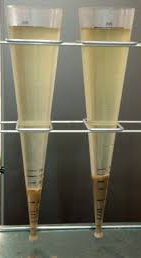
\includegraphics[scale=0.7]{ImhoffCone}\\
			      		Imhoff Cone\\
			      		\textit{Note the ml markings at the bottom of the cone}
			      		
			      		
			      	\end{center}
		      \end{minipage}
%			      \end{minipage}
			      	\item One factor which affects settleability is the conveyance time of the sewage to the treatment plant. 			
			      	\item The settleable component of the suspended solids will decrease as the sewage becomes more septic due to longer conveyance times.
			\item Influent and effluent total suspended solids are measured to establish the overall treatment and individual process efficiencies.  
			\item Volatile solids measurements before and after biological processes such as secondary treatment and digestion provide information on the process efficiency.\\
		\end{itemize}


	\subsubsection{Procedures for Solids Analysis}\index{Procedures for Solids Analysis}
% 		\begin{enumerate}%$$$$$$$$$$$$$$$$$$$$%
% 			\definecolor{shadecolor}{RGB}{220, 220, 220}
% 			\begin{snugshade*}
% 				\item \noindent\textsc{Procedures for Solids Analysis}
% 			\end{snugshade*}		
	\textbf{Determining wastewater suspended solids - Total(TSS) and Volatile(VSS) concentrations:}\\	
			% \begin{enumerate}[a.]
			% 	\definecolor{shadecolor}{RGB}{110, 192, 221}
			% 	\begin{snugshade*}
			% 		\item \noindent\textsc{Determining wastewater suspended solids - Total(TSS) and Volatile(VSS) concentrations:}
			% 	\end{snugshade*}
				 
				%\hl{How total suspended solids concentration is established for a wastewater sample:}
				\begin{itemize}
					\item A known volume of wastewater sample is filtered through a pre-weighed filter paper
					\item The suspended solids will be retained by the filter
					\item The water with the dissolved solids will pass through the filter
					\item The filter paper with the filter solids is rinsed with distilled water to remove 
					\item The filter paper with the solids is dried in the oven and then weighed
					\item The difference between the weight of the dried filter paper with the solids and the pre-weighed filter paper, measured in mg, will be the suspended solids in: mg per the original quantity of wastewater sample taken.  This value can be converted to give the suspended solids content in mg/l
					\item A filter paper with the dried solids is incinerated in a muffler furnace
					\item The difference in the weight of the solids, before and after incineration is the fixed solids
					\item The difference between the weight of the solids before incineration and the fixed solids is the volatile solids
				\end{itemize}
				
	\textbf{Determining wastewater and sludge total solids (TS) and volatile solids (VS) concentrations:}\\	
				
				% \begin{snugshade*}
				% 	\item \noindent\textsc{Determining wastewater and sludge total solids (TS) and volatile solids (VS) concentrations:}
				% \end{snugshade*}
				\begin{itemize}
					\item A certain quantity of wastewater (by volume) or sludge (by weight) is taken in a pre-weighed dish and weighed.  Note:  the sample is not filtered.
					\item The dish with the sample is dried in an oven
					\item The difference in the weight of the pre-weighed dish from that of the dish with the dried sample is the total solids
					\item The dried solids are incinerated in a muffler furnace
					\item The difference in the weight of the solids, before and after incineration is the fixed solids
					\item The difference between the fixed solids and the total solids is the volatile solids
					\item Total solids of a sludge sample is reported as a \% of the sludge weight.  A 7\% sludge has 7 lbs of solids for every 100 lbs of sludge.
				\end{itemize}
				
							
				
				
					\hl{For sludge samples, volatile solids is typically reported as the volatile solids fraction in \% of the total solids content of the sludge.  For example, if a 8\% sludge (i.e sludge which has 8\% TS or 80,000mg/l solids), is reported to have 70\% volatile, it means that 70\% of the total solids - 0.7*8\%=5.6\% or 56,000mg/l is the sludge volatile solids content.  \emph{70\% volatile does not meet the sludge has 700,000mg/l volatile solids}}\\
				
% 			\end{enumerate}
	\subsubsection{Summary of Wastewater Solids}\index{Summary of Wastewater Solids}		
% 			\begin{snugshade*}
% 				\item \noindent\textsc{Summary of Wastewater Solids}
% 			\end{snugshade*}
			\begin{itemize}
				\item Solids in wastewater can be categorized as dissolved or suspended
				      \begin{itemize}
				      	\item Suspended solids can be further categorized as settleable or unsettleable
				      \end{itemize}
				\item Solids can also be categorized as organic (aka: volatile) or inorganic (aka: fixed)
				\item Colloidial particles are small sized particles some of which pass through the filter and accounted as part of dissolved solids
				\item TSS - Total Suspended Solids are the solids that are captured on the filter paper upon filtration of the wastewater sample.  
				\item Wastewater samples typically analyzed for TSS include:  plant, primary and secondary processes - influent and effluent.  TSS is reported in mg/l
				\item TS - Total Solids are solids content of sludge.  TS of sludge is established by drying a preweighed quantity of sludge in an oven and is typically reported as \% solids - which is how many parts (by weight) of solids per 100 parts (by weight) of sludge.
				\item Volatile solids are solids that are removed when the solids are incinerated at 550C.  The solids that remain after incineration are fixed or non-volatile or inorganic solids.
			\end{itemize}
	\subsubsection{Wastewater Solids Content}\index{Wastewater Solids Content}			
% 			\begin{snugshade*}
% 				\item \noindent\textsc{Typical influent wastewater contains:}
% 			\end{snugshade*}
			\begin{itemize}
				\item Less than 0.1\% total solids.  Total solids concentration in typical wastewater is about 750mg/l
				\item The total solids are 50\% organic (volatile) and 50\% inorganic (fixed)
				\item Of the total solids, dissolved solids constitute about 70\% of the solids and the remaining 30\% solids are suspended solids
				\item 40\% of the dissolved solids are volatile the remaining 60\% are fixed
				\item 70\% of the suspended solids are volatile and the remaining 30\% are fixed
			\end{itemize}
			% \clearpage\thispagestyle{empty}
			\begin{figure}[!htbp]
			\vspace{2cm}
				\begin{center}
					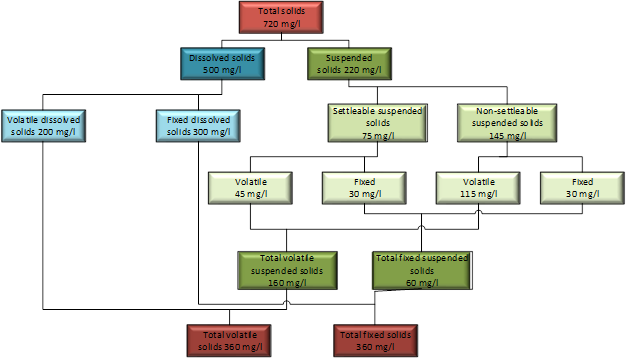
\includegraphics[scale=0.8]{WastewaterSolids}\\
					\caption{Typical Wastewater Solids Concentrations}
				\end{center}
				\end{figure}
% % 			\end{enumerate}
				
\subsection{Nutrients}\index{Nutrients}	
% 			\begin{snugshade*}
% 				\item \noindent\textsc{Nutrients}
% 			\end{snugshade*}	
			\begin{itemize}
				\item Plant nutrients - nitrogen and phosphorous, present in wastewater effluent discharge, promote growth of plant and algal matter in the receiving waters causing destruction of the normal aquatic life mainly due to oxygen depletion - eutrophication.
				      
				\item Because of the potential impacts of the presence of these nutrients in wastewater effluent on the receiving waters,  limits on the levels of these nutrients is typically stipulated in the treatment plant's wastewater discharge permit.
				      
				\item Typically, conventional secondary treatment processes are designed primarily remove the organics from the wastewater.  Secondary treatment process designed to additionally remove nutrients is deemed as tertiary or advanced treatment is termed as Biological Nutrient Removal (BNR).
			\end{itemize}
	\subsubsection{Nitrogen}\index{Nitrogen}				
% 			\begin{enumerate}%@@@@@@@@@@@@@@@@@@%
% 				\definecolor{shadecolor}{RGB}{220,220,220}
% 				\begin{snugshade*}
% 					\item \noindent\textsc{Nitrogen}%@@@@@@@@@@@@@@@@@@%
% 				\end{snugshade*}

	\textbf{Forms of nitrogen:}\\	
% 				\begin{itemize}
% 					\item Forms of nitrogen:\\
					      \begin{itemize}
					      	\item About 60\% of nitrogen in wastewater is present as ammonia nitrogen (about 60\%).  The ammonium nitrogen is present either in the form of ammonia (NH$_3$ ) or as ammonium (NH$_4^+$ ) ion.   These two forms can rapidly change from one to the other depending on pH and temperature.  Under low pH (acidic) or neutral conditions – pH less than or equal to 7, ammonia exists mostly as ammonium.  Ammonia becomes the dominant form as the pH increases to 8 and beyond.
					      	\item The other dominant form of nitrogen, about 40\% of the total nitrogen is as organic nitrogen
					      	\item Nitrogen measured as Total Kjeldahl Nitrogen (TKN) which is the sum of the organic nitrogen and the ammonia nitrogen concentrations.  Total inorganic nitrogen is the total concentration of ammonia nitrogen, NO3-, and NO2-.   Table provides the concentrations and forms of nitrogen in wastewater.
					      \end{itemize}
					      \setlength{\arrayrulewidth}{0.7mm}
					      \setlength{\tabcolsep}{8 pt}
					      \renewcommand{\arraystretch}{0.8}
					      \begin{center}
					      \begin{figure}[!htbp]
					      	\noindent \begin{tabular}[!htbp]{ |p{6cm}|p{2.0cm}|p{2.5cm}|p{2.cm}|}
					      	\hline
					      	\multicolumn{4}{|c|}{\textbf{Forms of Nitrogen in Wastewater}} \\
					      	\hline
					      	%\thead{A Head} & \thead{A Second \\ Head} & \thead{A Third \\ Head} \\
					      	%\hline%
					      	
					      	\hspace{1.8 cm}Forms of Nitrogen & \hspace{0.25 cm} Formula & \hspace{.4 cm} Found in & \hspace{.4 cm} Typical \newline \hspace{.2 cm}Concentration\\
					      	\hline
					      	\small Ammonia/Ammonium & \small NH$_3$/NH$_4^{\enspace +}$ &  \small Influent wastewater & 30-50 mg/l\\
					      	
					      	Total Kjeldahl Nitrogen \newline  \small (Ammonia/Ammonium + Organic Nitrogen) &  \small TKN &  \small Wastewater \newline  \small effluent  & 30-60 mg/l \\
					      	
					      	\small Total Inorganic Nitrogen \newline  \small (Ammonia/Ammonium + Nitrite + Nitrate) & \small TIN &  \small  Wastewater \newline  \small effluent  & 1-40 mg/l \\
					      	
					      	\small Nitrate  & $NO_3^{\enspace -}$ &  \small Nitrified effluent &  \small 1-35 mg/l \\
					      	
					      	\small Nitrate  &  $NO_2^{\enspace -}$ &  \small Partially nitrified effluent &  \small 0.1-2 mg/l \\
					      	
					      	\hline
					      	\end{tabular}
					      	\caption{Forms of Nitrogen}
					      	\end{figure}
					      \end{center}
					      
		\subsubsection{Phosphorous}\index{Phosphorous}			
		\textbf{Forms of phosphorous:}\\
					      \begin{itemize}
					      	\item The principal forms are organically bound phosphorus, polyphosphates, and orthophosphates.
					      	\item Organically bound phosphorus originates from body and food waste and, upon biological decomposition of these solids, is converted to orthophosphates. 
					      	\item Polyphosphates originate from synthetic detergents and are hydrolyzed to orthophosphates. Thus, the principal form of phosphorus in wastewater is assumed to be orthophosphates, although the other forms may exist. Orthophosphates consist of the negative ions PO$_4$$^{3-}$, HPO$_4$$^{2-}$, and H$_2$PO$_4$ $^-$.  These may form chemical combinations with cations (positively charged ions).
					      \end{itemize}

\subsection{Oil and Grease}\index{Oil and Grease}	
			Fats, oil and grease in wastewater originate from homes, food establishments and industries.
			\begin{itemize}
				\item Oil and grease content of wastewater is established in the laboratory by extracting it with a solvent - \textit{n}-hexane.  The concentration of oil and grease is reported in mg/l and typical oil and grease content of wastewater ranges from 80 - 120 mg/l
				\item Presence of excessive oils and grease could potentially impact the secondary treatment process
				\item Oils and grease are removed as floatables in primary treatment and sent with the sludge to the digesters
			\end{itemize}
		



\section{Wastewater Properties}\index{Wastewater Parameters}			
		Laboratory and field tests are conducted to measure parameters which are critical for monitoring and controlling treatment.  The following are the key parameters that are measured.	
			
\subsection{pH}\index{pH}	
			\hl{pH is a measure of the hydrogen ion (H$^+$) content or the acidity or basicity of a solution.}  pH impacts the chemical and micribiological elements of wastewater treatment processes and thus pH measurement and control is critical.
			\begin{itemize}
				\item Pure water dissociates into equal concentration of hydrogen ions and hydroxide ions:\\ 
				      $H_2O \rightarrow H^+ + OH^-$.
				\item The H$^+$ are responsible for acidic properties and the OH$^-$ ions for the basic properties.  
				\item pH is the inverse of H$^+$ concentration; pH increases when the concentration of H$^+$ decreases relative to the concentration of OH-. 
				\item pH scale ranges from 0 – 14. When the concentration of both H$^+$ and OH$^-$ are equal, as in pure water, it is considered neutral and its pH is 7.0.  \item If the pH of a sample solution is below 7.0, the sample is termed acidic and is alkaline or basic if its pH is above 7.0. 
				\item Each change of 1 pH unit represents a 10 fold change in concentration.  For example, a sample with a pH of 2.0 is 1000 times more acidic than a sample with a pH of 5.0. 
				\item pH is measured by an electrode that is sensitive only to H$^+$ or using a pH strip which is essentially an adsorbent paper which is pre-impregnated with chemicals which change color under different H$^+$ concentrations.
				\item Most organisms involved in biological wastewater treatment processes do well within a a narrow range of pH near neutral (pH of 7).			
			\end{itemize}
			
\subsection{Oxidation Reduction Potential (ORP)}\index{Oxidation Reduction Potential (ORP)}			
			\begin{itemize}
				\item ORP measurements are common in wastewater process control for monitoring conditions and process efficiency
				\item ORP is measured in milivolts (mV) using a probe\\
				\item ORP is a measure of the potential of oxidation/reduction – electron transfer, based chemical reactions to occur 
				\item If the measured ORP value (in mV), is positive it indicates an environment where oxidation will occur and if negative, an environment where reduction reactions will occur
				\item Higher positive value indicates a stronger oxidative environment and likewise, a lower (more negative) ORP value indicates a stronger reductive environment 
				\item For example, during chlorine disinfection, which is an oxidation process, the wastewater will exhibit a positive ORP.  Stronger the oxidative power of chlorine, higher will be the wastewater ORP value
				\item All living matter, including microbes depend upon respiration to generate energy and respiration involves series of chemical oxidation-reduction reactions 
				\item Bacteria grow and thrive only in specific chemical - oxidative-reductive environments which support its inbuilt metabolic pathways
				\item Aerobic bacteria need molecular oxygen as the terminal electron acceptor as part of its cellular respiration proces.  Bacteria adapted to exist in an environment where molecular oxygen is not present (anoxic and anaerobic), rely on electron acceptors such as NO$_3^-$ (denitrification), SO$_4^-$ (sulfide formation) and carbon (methane formers in anaerobic digestion)
				\item Aerobic bacteria responsible for cBOD removal in the secondary treatment process would be inhibited or wiped-out if the wastewater oxidation potential dropped and become reductive.  Likewise, if the wastewater in the sewer pipes which is normally of reductive (negative ORP)  was to become oxidative because of aeration (dissolving oxygen) it would cease the hydrogen slufide activity of the anaerobic bacteria
				\end{itemize}
		
			\setlength{\arrayrulewidth}{0.6mm}
			\setlength{\tabcolsep}{8 pt}
			\renewcommand{\arraystretch}{1.2}
			\begin{center}
			\begin{table}[!htbp]
				\begin{tabular}{ |p{9.5cm}|p{4.0cm}|}
					\hline
					\multicolumn{2}{|c|}{\textbf{Typical Wastewater Process ORPs}} \\
					\hline
					
					\hline
					\small Clorine disinfection & \small +650 to +700 mV  \\
					\small Nitrification & \small +100 to +350 mV   \\
					\small Biological phosphorous removal & \small +20 to +250mV        \\
					\small Activated sludge	cBOD degradation with free molecular oxygen & \small +50 to +250 mV  \\
					\small Denitrification                                              & \small +50 to -50 mV   \\
					\small Influent wastewater                                          & \small - 200 mV  \\ 
					\small Sulfide formation                                & \small -50 to -250 mV  \\
					\small Anaerobic Digestion: Acid formation (Acidogenesis)           & \small -100 to -225 mV \\
					\small Biological phosphorous removal & \small -100 to -250 mV \\
					\small Anaerobic Digestion: Methane production  (Methanogenesis)     & \small -75 to -400 mV  \\
					\hline
				\end{tabular}
	\end{table}			
			\end{center}
			
\subsection{Alkalinity}\index{Alkalinity}	
			\begin{itemize}
				\item \hl{Alkalinity is the ability of a water to neutralize acids.}  
				\item During certain wastewater treatment processes including anaerobic digestion, acids are generated as a result of microbiological activity.  The bacteria and other biological entities which play an active role in wastewater treatment are most effective at a neutral to slightly alkaline pH of 7 to 8.  In order to maintain these optimal pH conditions for biological activity there must be sufficient alkalinity present in the wastewater to neutralize acids generated by the active biomass.
				\item This ability to maintain the proper pH in the wastewater as it undergoes treatment is the reason why alkalinity is so important to the wastewater industry.
				\item The alkalinity is due to the presence of acid neutralizing bases in the water including the hydroxyl (OH$^-$), carbonate (CO$_3$$^-$) and bicarbonate (HCO$_3$$^-$)  ions.  These ions are of mineral origin and are also formed from carbon dioxide which comes from the atmosphere and from the microbial decomposition of organic material.  The resistance to pH change of the water will continue until all the alkalinity contributing ions are neutralized.  
				\item The pH of a water serves as a guide to the types of alkalinity present in the water but is unrelated to the alkalinity content of a water.  Important Note:  Alkalinity is a measure of the ability to neutralize acids whereas a solution is termed alkaline (or basic) if its pH greater than 7. 
				\item Alkalinity is expressed as milligrams per liter of CaCO$_3$
			\end{itemize}
			
\subsection{Dissolved Oxygen}\index{Dissolved Oxygen}	
			\begin{itemize}
				\item Dissolved oxygen (DO) is the concentration of oxygen dissolved in the wastewater sample and is typically measured in the field using a DO probe.  A titration based Winkler Test is used in the laboratory
				\item The \hl{presence of oxygen indicates an aerobic environment} where dissolved, free oxygen is available for aerobic microorganisms to live, BOD removal in the activated sludge process occurs as a result of the activity of aerobic bacteria.  The absence of DO indicates that the environment or condition is either anoxic or anaerobic.  
				\item \hl{In an anoxic environment, free oxygen is not present, but oxygen is available from its combined  forms - nitrate (NO$_3$ $^-$) and sulfate (SO$_4$ $^-$)} for the the consumption of microorganisms.  Example of an anoxic process is denitrification.  In denitrification, the anoxic bacteria in the presence of food (cBOD) consume the combined oxygen in nitrates (NO$_3$ $^-$ ) and convert it to nitrogen gas.
				\item \hl{The complete absence of oxygen including free and combined oxygen is an anaerobic environment.}
				\item Microorganisms are termed as obligate aerobes if they cannot survive without free oxygen.  Facultative aerobes are microorganisms which can survive in both aerobic and anaerobic environments.  
			\end{itemize}
			
\subsection{Microbiological testing and monitoring}\index{Microbiological testing and monitoring}	
			
			Microbes play a critical role in wastewater treatment.  
			\begin{itemize}
				\item Heterotrohic (organisms that consume organic material) microbes are responsible for the biological wastewater treatment processes - secondary treatment process, digestion and nutrient removal; and
				\item Pathogens - agents that cause disease are present in wastewater effluent.
			\end{itemize}
Microbiological testing and monitoring is conducted as part of the wastewater treatment typically for the following:
\begin{enumerate}[1.]
				
				\item Microbiological testing related to monitoring and troubleshooting biological wastewater treatment\\
				
				Microbes involved in biological wastewater treatment processes include:\\
				\begin{itemize}
					\item Fungi - Filamentous fungi occasionally bloom in activated sludge processes due to low pH or nutrient deficiency and cause problems with the settleability.
					\item Protozoa - Protozoas play a important role in the secondary treatment process.  Common protozoas in the activated sludge process include:
					      \begin{itemize}
					      	\item Amoeba
					      	\item Flagellate
					      	\item Cilliate
					      \end{itemize}
					\item Rotifers
					\item Nematodes
					\item Bacteria - Bacteria is the predominant microorganism responsible for the biological wastewater water treatment.  
				\end{itemize}
				\begin{itemize}
					\item The effectiveness of the biological wastewater treatment processes is primarily due to the presence of a microbial ecosystem with a right balance of populations of different microbial species.
					\item Methods used for monitoring the microbial composition include direct monitoring using a light microscope to see which and how many of the different microbial species are present - typically used for activated sludge process.
					\item Indirect method includes monitoring other parameters such as pH and alkalinity which are influenced by microbiological activity.
					\item The microbial monitoring ensures process stability and helps identify potential process upset conditions caused by changes to the microbial population due to other external factors - toxicty, organic loading, temperature etc.
				\end{itemize}

\item Microbiological testing related to monitoring and controlling pathogens in treated wastewater effluent\\

	
				Pathogens in wastewater belong to the following groups:
				\begin{itemize}
					\item Bacteria:  Although, bacteria is present in large numbers in feces, pathogenic or bacteria are present only because of an infection and this pathogenic bacteria can potentially spread the infection to other healthy individuals.  Disease spread by pathogenic bacteria include diarrhea, cholera and typhoid among many others.
					      
					\item Viruses: A large number of viruses may infect humans and are present in feces.  These include enteroviruses (including polioviruses), hepatitis A virus, reoviruses and diarrhea-causing viruses (especially rotavirus).
					      
					\item Protozoa:  Many species of protozoa can infect humans and cause diarrhoea and dysentery. Girardia which casues diarrheal illness is an example of a protozoan pathogen
					      
					\item Helminths:  These are parasitic worms that can infect humans and are transmitted to others through its eggs or larval forms
					      
				\end{itemize}
				
				\begin{itemize}
					\item As one of the main reasons for treating wastewater is to protect public health, microbiological/pathogen testing of the wastewater effluent and the surface water impacted by the wastewater discharge is conducted to meet the requirements of a wastewater discharge permit, to monitor the pathogen impact of treated wastewater discharge and assess the level of contamination of a public body of water.
					\item The bacteriological tests involves detection and quantification of one or more of the following bacteria:  total coliforms, fecal coliforms, E. Coli, and Enterococcus.  
					      \begin{itemize}
					      	\item The main reason why these bacteria such as coliforms and enterococcus are used \hl{as it is not practical to detect and quantify all pathogens associated with wastewater.}  
					      	\item These selected bacteria originate from feces and indicate fecal contamination and thus serve as an indicator organisms for pathogens of wastewater origin.  
					      	\item Also, they are abundant, potentially less harmful, and easy to detect.  E. coli has been shown to be a better predictor of the potential for impacts to human health and therefore many newer wastewater discharge permits require E. Coli testing in lieu of fecal coliform testing requirements.
					      \end{itemize}
					\item The microbiological test sample is always collected as a grab in a clean, sterile borosilicate glass or plastic bottle containing sodium thiosulfate. 
					      \begin{itemize}
					      	\item Sodium thiosulfate is added to remove residual chlorine which will kill coliforms during transit. 
					      	\item If the sample is not preserved or maintained under proper conditions until the test is conducted in the laboratory, the test would provide erroneous results.
					      	\item Samples must be refrigerated if they cannot be analyzed within 1 hour of collection and must be handled with care to prevent contamination and adverse conditions such as prolonged exposure to direct sunlight.
					      	\item The maximum holding time for state or federal permit reporting purposes is 6 hours. 
					      \end{itemize} 
					\item As it is not possible to exactly quantify the number of bacteria present, a statistical based - \hl{Most Probable Number (MPN)} approach is utilized.  The methods for wastewater bacteriological tests include:  multiple-tube fermentation technique, membrane filtration and quanti-tray testing. 
				\end{itemize}
			\end{enumerate}

\subsection{Specific Gravity}\index{Specific Gravity}				
			\begin{itemize}
				\item Specific gravity is a term to express the weight of a solution with respect to that of water
				\item Water weighs 1 kg/L or 8.34 lbs/gallon or 62.4 lbs/ft$^3$
				\item A solution with a specific gravity of 1.2 will weigh 1.2 times the same volume of water.  1 L of that solution will weigh ( 1.2 kg )/L  or  ( 1.2*8.34=10lbs )/gallon.
				\item Typically wastewater and the associated unthickened sludge, for all practical purposes is assumed to have a specific gravity of 1 - implying 8.34 lbs/gallon.
				\item Specific gravity is typically used for calculations related to chemicals used in wastewater treatment.
			\end{itemize}
\chapterimage{SamplingCoverBW.png}
\chapter{Wastewater Sampling}		
\section{Wastewater Sampling}\index{Wastewater Sampling}
		\begin{itemize}
			\item Field or laboratory measurement of a certain parameter is critical in wastewater treatment operations to obtain information about wastewater characteristics in order to either characterize a wastewater stream, or to monitor a treatment process or for permit compliance.  
			\item A sample is a small part of the whole representing the whole.  Thus, a sample needs to be such that it truly represents the entire population – which in a wastewater operations could be either a wastewater stream, wastewater solids or a chemical used.
		\end{itemize}
		
\subsection{Sampling Methods}\index{Sampling Methods}
\subsubsection{Grab Samples}\index{Grab Samples}
				\begin{itemize}
					\item A grab sample is a sample collected at a specific spot at a site over a short period of time.  
					\item Grab sampling allows for instantaneous analysis of parameters such as pH, dissolved oxygen, chlorine residual, temperature and other parameters which change rapidly with time.
					\item A grab sample represents a snapshot of space and time of a process stream.
					\end{itemize}
\subsubsection{Composite Samples}\index{Composite Samples}
				\begin{itemize}
					\item A composite sample is a collection of discrete samples are combined over a certain period or space and therefore represent the average performance of a wastewater treatment plant or a process during the collection period.\\  
					\item Composite sampling can be either based on:
					      
					      1. constant time interval (time proportioned sampling)\\
					      2. constant wastewater volume interval (flow-proportioned sampling), and\\
					      3. treatment process space - includes samples taken at different depths\\
					      
					\item Composite samples are typically collected using automated samplers which can be programmed to collect samples at pre-established time intervals – for time proportional sampling.
					\item Time and space composite samples are collected by adding equal volumes of samples collected from different times or locations.  
					\item Flow proportional composite samples comprise of volume of each subsample based on flow.\\  
				\end{itemize}
				
			\begin{center}
				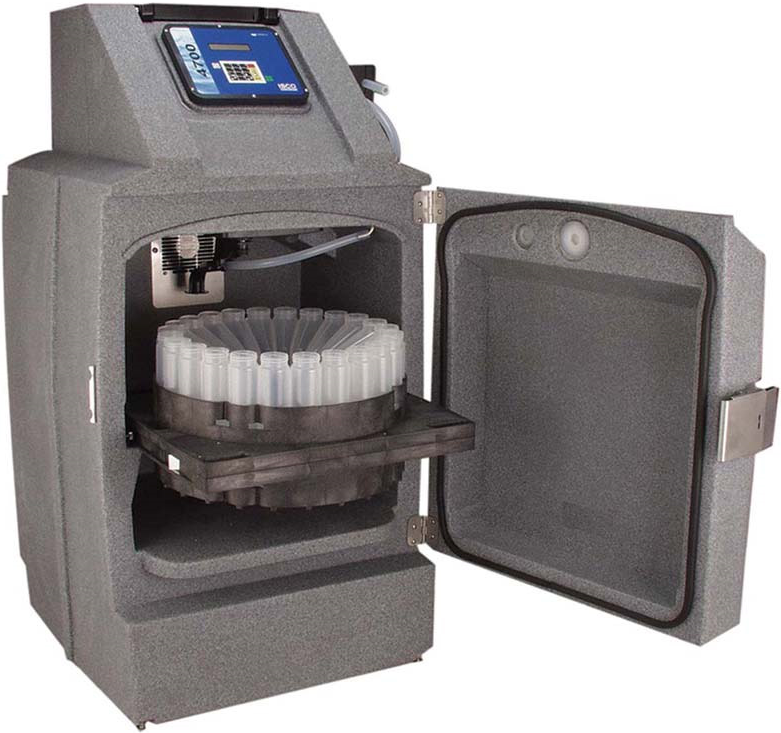
\includegraphics[scale=0.2]{Autosampler} \hspace{2cm} 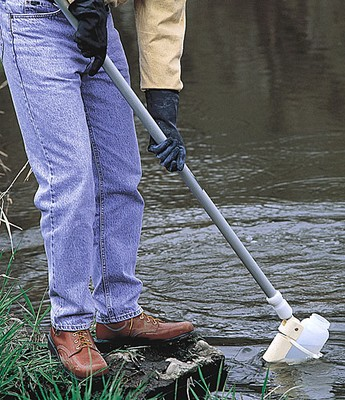
\includegraphics[scale=0.37]{Grabsampler}\\
			\end{center}
			\hspace{2.3cm} Automated Sampler \hspace{2.0cm} \parbox{\textwidth}{Grab Sampling Using a Long Handle Dipper}\\

\subsubsection{Sampling Precautions and Protocols}\index{Sampling Precautions and Protocols}
			\begin{itemize}
				\item Samples should represent the major portion of the process or the process stream and should be taken from places where the mixing is thorough, avoiding dead spots and areas of heavier or lighter loadings. 
				\item The collected sample is invariably exposed to conditions very different from the original source and is subject to change due to chemical and microbiological activity.  
				\item Thus, in order to ensure integrity of sample, sample preservation techniques specific to the analysis to be performed is needed.  
				      \begin{itemize}
				      	\item The preservation technique should not only allow for stabilizing the parameter to be analyzed, it should also not interfere with the analyses.  
				      	\item The common preservation techniques involve use of proper containers, temperature control, addition of chemical preservatives, and observance of the recommended maximum sample holding time.
				      \end{itemize}
			\end{itemize}

\section{Data Reporting}\index{Data Reporting}	
		\begin{itemize}
			\item Arithmetic mean is typically calculated for reporting data where multiple samples have been collected and analyzed for the same process stream at different times and for reporting average value over a certain time period – daily, monthly etc.\\ \item Arithmetic mean mathematically is calculated by adding all the result values and dividing by the total number of data points.\\
		\end{itemize}
		Mathematically the arithmetic mean is represented as:\\
		$$\bar{x}=\frac{\sum_{i=1}^{n} x^i}{n} = \frac{x_1+x_2+x_3...x_n}{n}$$
		For example:\\
		Arithmetic mean of the following set of data points:  200, 304, 250, 400 is calculated as:\\
		\vspace{10pt}
		Arithmetic Mean = $\frac{200 + 302 + 250 + 400}{4}= 288$\\
		\vspace{10pt}
		For data sets for analysis such as fecal coliform could include values which vary by several orders of magnitudes, using the arithmetic mean to report the average value is not appropriate as the lower or higher values would bias the calculated mean.\\
		\vspace{10pt}
		For example, consider a data set with values:  260, 300, 500, 5,000, 320 and 200.\\
		\vspace{10pt}
		The arithmetic mean = $\frac{260+300+500+5,000+320+200}{6} = 3,444$\\
		Here the 5000 value completely skews the arithmetic mean.
		
		Therefore, for such tests, the geometric mean calculation is used for reporting the average value.\\
		
		
		Mathematically a geometric mean is represented as:\\
		$$\Bigg(\prod_{i=a}^n\Bigg)^{\frac{1}{n}}=\sqrt[n]{a_1*a_2*a_3...a_n}$$
		 
		Calculation method:\\
		1.	Find the product of all the data points (analogous to first calculating the sum of all the data points when calculating the arithmetic mean)\\
		260*300*500*5,000*320*200 = 12,480,000,000,000,000\\
		2.	Raise the product to the inverse of the number of data points\\
		(*Using the power function of a scientific calculator)\\
		Here n (\# data points) = 6 $\implies$ geometric mean = $(12,480,000,000,000,000)^{\frac{1}{6}}   = 482$

\chapterimage{Collections.jpg} % Chapter heading image

\chapter{Collections}






The collection system resembles a tree that branches out from the treatment plant to collect the wastewater from individual sources.

\section{Wastewater Collection Piping}\index{Wastewater Collection Piping}	
	\begin{itemize}
		\item A \hl{lateral} is the piping that connects the public sewer to the building. 
		\item Laterals flow into larger lines called \hl{mains}.
		\item Mains carry the flow into the largest lines in the system, called \hl{trunk lines}. 
		\item A trunk line is the pipe that brings water into the treatment plant.
	\end{itemize}
\section{Sanitary Sewer Systems}\index{Sanitary Sewer Systems}

Sanitary sewer systems collect and convey wastewater from residential, commercial and industrial sources to a centralized wastewater treatment facility for treatment. 

\subsection{Storm-water systems}\index{Storm-water systems}

Storm-water systems are designed solely for the conveyance of storm-waters waters directly to streams, rivers, lakes, or the ocean.
 
\subsection{Combined sewer systems}\index{Combined sewer systems}
\begin{itemize}
\item Combined sewer systems collect and convey sanitary sewage and urban runoff in a common piping system.
\item Combined sewers could potentially cause serious water pollution problems during combined sewer overflow (CSO) events when wet weather flows exceed the sewage treatment plant capacity.
	\end{itemize}
\begin{center}
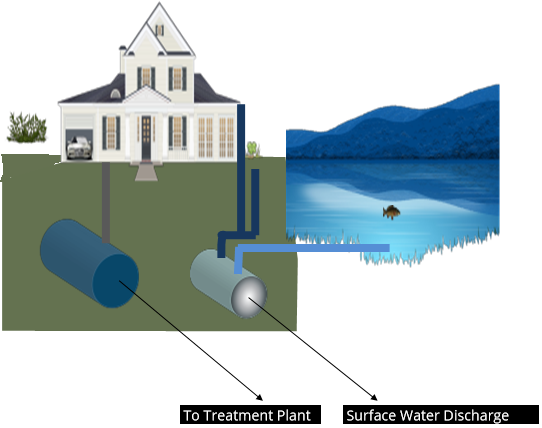
\includegraphics[scale=0.45]{SeperatedSystem1} \hspace{1 cm} 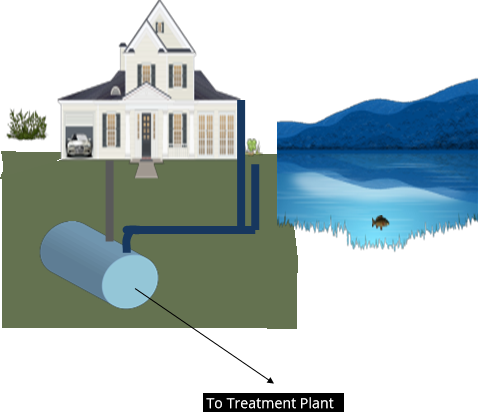
\includegraphics[scale=0.45]{CombinedSystem1}
\end{center}
			\hspace{2.6cm} Separated System \hspace{3.2cm} \parbox{\textwidth}{Combined System}\\

\section{Collections Systems Basics}\index{Collections Systems Basics}
	\begin{itemize}
\item The primary type of a collection system is a \hl{gravity system}. A gravity system is so named because the wastewater flows down gradient in the sewer, driven by forces of gravity. 
\item The collection system includes the gravity sewers, force mains, manholes, pumping equipment, and other facilities that collect and convey the water to a wastewater treatment plant. 
\item Sewers are generally laid at a minimum slope to ensure open channel flow through the pipe at a \hl{minimum velocity of 2.0 feet per second}. The minimum velocity is required to ensure that solids do not settle out in the sewer.  
\item When the sewer lines reach a certain depth, the flow must be lifted back through a lift or pump station.  
\item \hl{Lift stations} are built whenever wastewater must be pumped to a higher altitude, whether it's to lift water up so that it can gravity flow or to pump it over a rise or hill.  
\item The discharge from the pump station may be to another gravity sewer at that location or through a pressurized force main. 
\item Key elements of lift stations include a wastewater receiving well (wet-well), pumps and piping with associated valves.
\item The size of the wet well affects the operating of the station. If a wet well is too small, excessive starting and stopping of the pump motors will occur, resulting in premature failure. If the wet well is too large, solids will tend to settle on the bottom, blocking the pump suction line and leading to the generation of hydrogen sulfide and methane.
\item The dry well is the portion of the dry well/wet well pumping station that houses the necessary equipment required to pump the wastewater. The dry well is so named because it is isolated from the incoming wastewater.
\item Centrifugal pumps are the most common type of pump found in wastewater pumping stations. 
\item In the USA, wastewater generated in a typical home is about 70 gal/day/person
\end{itemize}

\section{Collections Related Operational Issues}\index{Collections Related Operational Issues}
Infiltration and inflow (I/I) is the unwanted flow into the wastewater collections systems.
\subsection{Infiltration}\index{Infiltration}
\begin{itemize} 
\item Groundwater entering sanitary sewers through defective pipe joints and broken pipes is called infiltration. \hl{Remember:  \textbf{ground filters}}
\end{itemize}

\subsection{Inflow}\index{Inflow}
\begin{itemize} 
\item During rainstorms or snow thaws, large volumes of water may flow into the wastewater collections systems through leaky manhole covers or combined storm-water /wastewater connections.  In addition, private residences may have roof, cellar, yard, area, or foundation drains inappropriately connected to sanitary sewers.  These flows are termed as inflows. \hl{Remember: \textbf{rain flow}}
\end{itemize}

\textbf{Implications of I/I:}\\%$$$$$$$$$$$$$$$$$$$$%
\begin{itemize}
\item I/I decrease the efficiency and capacity of wastewater collection systems and treatment systems 
\item I/I can advance the need for capital costs to manage and treat flows
\item I/I contribute to the hydraulic overloading of treatment processes, which can affect public health and the compliance with NPDES permit requirements
\item I/I could cause Sanitary and combined sewer overflows(SSOs and CSOs) when wastewater flow volumes exceed the design capacity of the treatment plant 
\item I/I increase collection system and treatment facility operating costs
\end{itemize}

\subsection{Odors}\index{Odors}
\begin{itemize}
\item Hydrogen sulfide (H$_2$S), its associated compounds and methane are generated due to microbial

 activity in wastewater and the conveyance systems.  The \hl{rotten egg like smell} of hydrogen sulfide causes public nuisance odors, poses a health hazard for collections systems workers and causes corrosion of the system through its conversion to sulfuric acid.  The hydrogen sulfide generation is typically controlled by reducing the potential for septicity in wastewater through proper design of the system -  adequate velocities and adequate air space and through chemical treatment.
 \end{itemize}

\subsection{Fats, Oils and Grease (FOG)}\index{Fats, Oils and Grease (FOG)}
\begin{itemize}
\item FOG from food home, food establishments and industries affect the operation of the collection system
\item FOG has a tendency to accumulate in sewer pipes decreasing its wastewater carrying capacity.
\item Excessive FOG accumulation may cause sewer overflows
 \end{itemize}
 
\chapterimage{QuizIcon.jpg}
\chapter{Week 2 Module Assessment Quiz}

1. A lateral is the largest sewer line which brings the wastewater to the treatment plant\\

a. True \\
b. False \\
\vspace{0.5cm}

2. Total solids are made up of dissolved and suspended solids both of which contain organic and inorganic matter\\

a. True\\ 
b. False \\
\vspace{0.5cm}


3. A 24-hr flow proportioned sample may be collected for a fecal coliform test\\

a. True \\
b. False \\
\vspace{0.5cm}


4. Inflow is storm water entering into the sewer system\\

a. True \\
b. False \\
\vspace{0.5cm}


5. Fats, oils and grease accumulation in sewers can cause sewer overflows\\

a. True \\
b. False \\

\vspace{0.5cm}

6. A sewer system designed to transport only wastewater from homes, industries, institutions and businesses is called:\\

a. Combined sewer \\
b. Sanitary sewer \\
c. Service sewer \\
d. Building sewer \\

\vspace{0.5cm}

7. A device called an Imhoff cone is commonly used to measure settleable solids in:\\

a. \% \\
b. mL/L \\
c. mg/L \\
d. ppm \\
e. SVI units \\

\vspace{0.5cm}

8. An aerobic treatment process is one that requires the presence of:\\

a. Ozone \\
b. organic oxygen \\
c. no oxygen \\
d. combined oxygen \\
e. dissolved oxygen \\

\vspace{0.5cm}

9. Sludge solids in wastewater has an average specific gravity of 1.2; this means they are\\

a. 12\% heavier than water \\
b. 20\% heavier than water \\
c. 2\% lighter than water \\
d. 20\% lighter than water \\

\vspace{0.5cm}

10. Positive ORP indicates the presence of an $\rule{1cm}{0.15mm}$ environment

a. Oxidative \\
b. Reductive \\
c. Anaerobic \\
d. Toxic. \\
\vspace{2cm}
\textbf{Answers:}\\
1.	b. \\ 

\vspace{0.5cm}

2.	a. \\ 

\vspace{0.5cm}

3.	b.  \\
\vspace{0.5cm}


4.	a.  \\
\vspace{0.5cm}


5.	a.  \\
\vspace{0.5cm}


6.	b.  \\
\vspace{0.5cm}


7.	b.  \\

\vspace{0.5cm}

8.	e.  \\








					      
					% \item Nitrogen removal as part of the secondary treatment mainly involves nitrification-denitrification processes which involve conversion of ammonia nitrogen to nitrogen gas.
					      
% 				\end{itemize}
% 				\begin{snugshade*}
% 					\item \noindent\textsc{Phosphorous}
% 				\end{snugshade*}
% 				\begin{itemize}
% 					\item Forms of phosphorous:\\
% 					      \begin{itemize}
% 					      	\item The principal forms are organically bound phosphorus, polyphosphates, and orthophosphates.
% 					      	\item Organically bound phosphorus originates from body and food waste and, upon biological decomposition of these solids, is converted to orthophosphates. 
% 					      	\item Polyphosphates originate from synthetic detergents and are hydrolyzed to orthophosphates. Thus, the principal form of phosphorus in wastewater is assumed to be orthophosphates, although the other forms may exist. Orthophosphates consist of the negative ions PO$_4$$^{3-}$, HPO$_4$$^{2-}$, and H$_2$PO$_4$ $^-$.  These may form chemical combinations with cations (positively charged ions).
% 					      \end{itemize}
% 					\item Phosphorous removal in wastewater is typically accomplished by:
% 					      \begin{itemize}
% 					      	\item Biological uptake which utilizes specific phosphorous accumulating bacteria, and 
% 					      	\item Chemical precipitation
% 					      \end{itemize}
% 				\end{itemize}
% 			\end{enumerate}%@@@@@@@@@@@@@@@@@@%
% 			\pagebreak	
% 			\begin{snugshade*}
% 				\item \noindent\textsc{Oil and Grease}
% 			\end{snugshade*}
% 			Fats, oil and grease in wastewater originate from homes, food establishments and industries.
% 			\begin{itemize}
% 				\item Oil and grease content of wastewater is established in the laboratory by extracting it with a solvent - \textit{n}-hexane.  The concentration of oil and grease is reported in mg/l and typical oil and grease content of wastewater ranges from 80 - 120 mg/l
% 				\item Presence of excessive oils and grease could potentially impact the secondary treatment process
% 				\item Oils and grease are removed as floatables in primary treatment and sent with the sludge to the digesters
% 			\end{itemize}
% 	\end{enumerate}			
				
% 		%______________%
		
% 		\pagebreak
% 		\begin{snugshade*}
% 			\item \noindent\textsc{Wastewater Sampling}\\%$$$$$$$$$$$$$$$$$$$$%
% 		\end{snugshade*}
% 		\begin{itemize}
% 			\item Field or laboratory measurement of a certain parameter is critical in wastewater treatment operations to obtain information about wastewater characteristics in order to either characterize a wastewater stream, or to monitor a treatment process or for permit compliance.  
% 			\item A sample is a small part of the whole representing the whole.  Thus, a sample needs to be such that it truly represents the entire population – which in a wastewater operations could be either a wastewater stream, wastewater solids or a chemical used.
% 		\end{itemize}
		
% 		\begin{enumerate}[A.]
% 			\definecolor{shadecolor}{RGB}{225, 235, 235}
% 			\begin{snugshade*}
% 				\item \noindent\textsc{Sampling Methods:}\\%$$$$$$$$$$$$$$$$$$$$%
% 			\end{snugshade*}
			
% 			\begin{enumerate}[i.
% ]				\definecolor{shadecolor}{RGB}{220, 220, 220}
% 				\begin{snugshade*}
% 					\item \noindent\textsc{Grab Sampling}
% 				\end{snugshade*}
% 				\begin{itemize}
% 					\item A grab sample is a sample collected at a specific spot at a site over a short period of time.  
% 					\item Grab sampling allows for instantaneous analysis of parameters such as pH, dissolved oxygen, chlorine residual, temperature and other parameters which change rapidly with time.
% 					\item A grab sample represents a snapshot of space and time of a process stream. 
% 				\end{itemize}
% 				\begin{snugshade*}
% 					\item \noindent\textsc{Composite Sampling}
% 				\end{snugshade*}
% 				\begin{itemize}
% 					\item A composite sample is a collection of discrete samples are combined over a certain period or space and therefore represent the average performance of a wastewater treatment plant or a process during the collection period.\\  
% 					\item Composite sampling can be either based on:
					      
% 					      1. constant time interval (time proportioned sampling)\\
% 					      2. constant wastewater volume interval (flow-proportioned sampling), and\\
% 					      3. treatment process space - includes samples taken at different depths\\
					      
% 					\item Composite samples are typically collected using automated samplers which can be programmed to collect samples at pre-established time intervals – for time proportional sampling.
% 					\item Time and space composite samples are collected by adding equal volumes of samples collected from different times or locations.  
% 					\item Flow proportional composite samples comprise of volume of each subsample based on flow.\\  
% 				\end{itemize}
				
% 			\end{enumerate}
% 			\begin{center}
% 				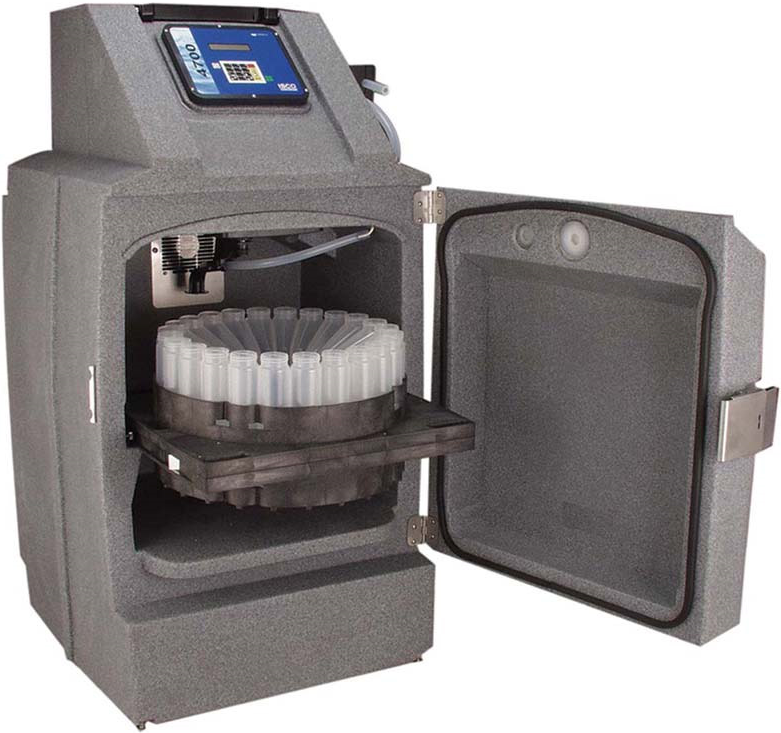
\includegraphics[scale=0.2]{Autosampler} \hspace{2cm} 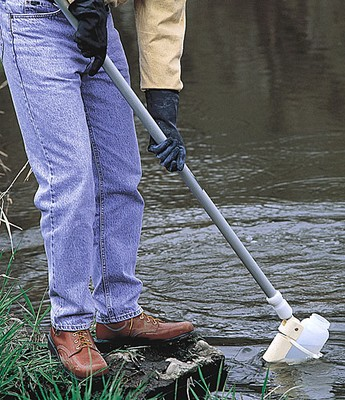
\includegraphics[scale=0.37]{Grabsampler}\\
% 			\end{center}
% 			\hspace{2.3cm} Automated Sampler \hspace{2.0cm} \parbox{\textwidth}{Grab Sampling Using a Long Handle Dipper}\\
% 			\begin{snugshade*}
% 				\item \noindent\textsc{Sampling Precautions and Protocols::}\\%$$$$$$$$$$$$$$$$$$$$%
% 			\end{snugshade*}
% 			\begin{itemize}
% 				\item Samples should represent the major portion of the process or the process stream and should be taken from places where the mixing is thorough, avoiding dead spots and areas of heavier or lighter loadings. 
% 				\item The collected sample is invariably exposed to conditions very different from the original source and is subject to change due to chemical and microbiological activity.  
% 				\item Thus, in order to ensure integrity of sample, sample preservation techniques specific to the analysis to be performed is needed.  
% 				      \begin{itemize}
% 				      	\item The preservation technique should not only allow for stabilizing the parameter to be analyzed, it should also not interfere with the analyses.  
% 				      	\item The common preservation techniques involve use of proper containers, temperature control, addition of chemical preservatives, and observance of the recommended maximum sample holding time.
% 				      \end{itemize}
% 			\end{itemize}
% 		\end{enumerate}
		

% 	\begin{snugshade*}
% 		\item \noindent\textsc{Wastewater Parameters}%$$$$$$$$$$$$$$$$$$$$%
% 	\end{snugshade*}
% 		Laboratory and field tests are conducted to measure parameters which are critical for monitoring and controlling treatment.  The following are the key parameters that are measured.	
			
% 		\begin{enumerate}[A.]
% 			\definecolor{shadecolor}{RGB}{225, 235, 235}
% 			\begin{snugshade*}
% 				\item \normalsize{\textbf{pH}}
% 			\end{snugshade*}
% 			\hl{pH is a measure of the hydrogen ion (H$^+$) content or the acidity or basicity of a solution.}  pH impacts the chemical and micribiological elements of wastewater treatment processes and thus pH measurement and control is critical.
% 			\begin{itemize}
% 				\item Pure water dissociates into equal concentration of hydrogen ions and hydroxide ions:\\ 
% 				      H$_2$O → H+ + OH$^-$.
% 				\item The H$^+$ are responsible for acidic properties and the OH$^-$ ions for the basic properties.  
% 				\item pH is the inverse of H$^+$ concentration; pH increases when the concentration of H$^+$ decreases relative to the concentration of OH-. 
% 				\item pH scale ranges from 0 – 14. When the concentration of both H$^+$ and OH$^-$ are equal, as in pure water, it is considered neutral and its pH is 7.0.  \item If the pH of a sample solution is below 7.0, the sample is termed acidic and is alkaline or basic if its pH is above 7.0. 
% 				\item Each change of 1 pH unit represents a 10 fold change in concentration.  For example, a sample with a pH of 2.0 is 1000 times more acidic than a sample with a pH of 5.0. 
% 				\item pH is measured by an electrode that is sensitive only to H$^+$ or using a pH strip which is essentially an adsorbent paper which is pre-impregnated with chemicals which change color under different H$^+$ concentrations.
% 				\item Most organisms involved in biological wastewater treatment processes do well within a a narrow range of pH near neutral (pH of 7).			
% 			\end{itemize}
			
% 			\begin{snugshade*}
% 				\item \noindent\textsc{ Oxidation Reduction Potential (ORP):}
% 			\end{snugshade*}
% 			ORP is a measure of the potential of a wastewater to allow for microbiological oxidation and reduction reactions.\\
% 			An example of wastewater treatment process where microbiological oxidation involved include the activated sludge process.  Whereas, anaerobic digestion is a microbiological reduction based process.
% 			\begin{itemize}
% 				\item ORP value is measured in millivolts (mV), using an electrochemical probe
% 				\item The measured ORP value provides an indication of the potential of oxidation and reduction reactions in that sample.
% 				\item A higher positive ORP is indicative of oxidation potential of the wastewater whereas a negative ORP value indicates potential for a reduction reaction to occur.
% 				\item ORP measurements are used for controlling treatment processes including nitrification, odor control and disinfection.  For example, in the disinfection process utilizing chlorine (bleach), ORP measurements provides the strength of the oxidation potential of chlorine present in the wastewater being disinfected.  This measurement is used for precisely controlling the chlorine dosing.  The proper chlorine control results in optimizing chlorine dosing which reduces potential toxicity issues and dechlorination costs.
% 			\end{itemize}
% 			Typical ORP applications include the following processes and process elements
			
			
% 			\setlength{\arrayrulewidth}{0.3mm}
% 			\setlength{\tabcolsep}{8 pt}
% 			\renewcommand{\arraystretch}{0.8}
% 			\begin{center}
% 				\begin{tabular}{ |p{9.5cm}|p{4.0cm}|}
% 					\hline
% 					\multicolumn{2}{|c|}{\textbf{Typical Wastewater Process ORPs}} \\
% 					\hline
					
% 					\hline
% 					\small Collections	Sulfide formation                                & \small -50 to -250 mV  \\
% 					\small Influent wastewater                                          & \small - 200 mV        \\
% 					\small Activated sludge	cBOD degradation with free molecular oxygen & \small +50 to +250 mV  \\
% 					\small Biological phosphorous removal                               & \small +25 to +250 mV  \\
% 					\small Denitrification                                              & \small +50 to -50 mV   \\
% 					\small Anaerobic Digestion: Acid formation (Acidogenesis)           & \small -100 to -225 mV \\
% 					\small Anaerobic Digestion: Methane production (Methanogenesis)     & \small -75 to -400 mV  \\
% 					\hline
% 				\end{tabular}
				
% 			\end{center}
			
% 			\begin{snugshade*}
% 				\item \noindent\textsc{Alkalinity}
% 			\end{snugshade*}
% 			\begin{itemize}
% 				\item \hl{Alkalinity is the ability of a water to neutralize acids.}  
% 				\item During certain wastewater treatment processes including anaerobic digestion, acids are generated as a result of microbiological activity.  The bacteria and other biological entities which play an active role in wastewater treatment are most effective at a neutral to slightly alkaline pH of 7 to 8.  In order to maintain these optimal pH conditions for biological activity there must be sufficient alkalinity present in the wastewater to neutralize acids generated by the active biomass.
% 				\item This ability to maintain the proper pH in the wastewater as it undergoes treatment is the reason why alkalinity is so important to the wastewater industry.
% 				\item The alkalinity is due to the presence of acid neutralizing bases in the water including the hydroxyl (OH$^-$), carbonate (CO$_3$$^-$) and bicarbonate (HCO$_3$$^-$)  ions.  These ions are of mineral origin and are also formed from carbon dioxide which comes from the atmosphere and from the microbial decomposition of organic material.  The resistance to pH change of the water will continue until all the alkalinity contributing ions are neutralized.  
% 				\item The pH of a water serves as a guide to the types of alkalinity present in the water but is unrelated to the alkalinity content of a water.  Important Note:  Alkalinity is a measure of the ability to neutralize acids whereas a solution is termed alkaline (or basic) if its pH greater than 7. 
% 				\item Alkalinity is expressed as milligrams per liter of CaCO$_3$
% 			\end{itemize}
			
% 			\begin{snugshade*}
% 				\item \noindent\textsc{Dissolved oxygen:}
% 			\end{snugshade*}
% 			\begin{itemize}
% 				\item Dissolved oxygen (DO) is the concentration of oxygen dissolved in the wastewater sample and is typically measured in the field using a DO probe.  A titration based Winkler Test is used in the laboratory
% 				\item The \hl{presence of oxygen indicates an aerobic environment} where dissolved, free oxygen is available for aerobic microorganisms to live, BOD removal in the activated sludge process occurs as a result of the activity of aerobic bacteria.  The absence of DO indicates that the environment or condition is either anoxic or anaerobic.  
% 				\item \hl{In an anoxic environment, free oxygen is not present, but oxygen is available from its combined  forms - nitrate (NO$_3$ $^-$) and sulfate (SO$_4$ $^-$)} for the the consumption of microorganisms.  Example of an anoxic process is denitrification.  In denitrification, the anoxic bacteria in the presence of food (cBOD) consume the combined oxygen in nitrates (NO$_3$ $^-$ ) and convert it to nitrogen gas.
% 				\item \hl{The complete absence of oxygen including free and combined oxygen is an anaerobic environment.}
% 				\item Microorganisms are termed as obligate aerobes if they cannot survive without free oxygen.  Facultative aerobes are microorganisms which can survive in both aerobic and anaerobic environments.  
% 			\end{itemize}
% 			\begin{snugshade*}
% 				\item \noindent\textsc{Microbiological testing and monitoring:}
% 			\end{snugshade*}
% 			Microbiological testing and monitoring is conducted as part of the wastewater treatment for two main reasons:
% 			\begin{enumerate}[1.]
% 				\item Heterotrohic (organisms that consume organic material) microbes are responsible for the biological wastewater treatment processes - secondary treatment process, digestion and nutrient removal; and
% 				\item Pathogens - agents that cause disease are present in wastewater effluent.
% 			\end{enumerate}
% 			\begin{enumerate}
% 				\definecolor{shadecolor}{RGB}{220, 220, 220}
% 				\begin{snugshade*}
% 					\item \noindent\textsc{Microbiological testing related to monitoring and troubleshooting biological wastewater treatment:}\\
% 				\end{snugshade*}
				
% 				Microbes involved in biological wastewater treatment processes include:\\
% 				\begin{itemize}
% 					\item Fungi - Filamentous fungi occasionally bloom in activated sludge processes due to low pH or nutrient deficiency and cause problems with the settleability.
% 					\item Protozoa - Protozoas play a important role in the secondary treatment process.  Common protozoas in the activated sludge process include:
% 					      \begin{itemize}
% 					      	\item Amoeba
% 					      	\item Flagellate
% 					      	\item Cilliate
% 					      \end{itemize}
% 					\item Rotifers
% 					\item Nematodes
% 					\item Bacteria - Bacteria is the predominant microorganism responsible for the biological wastewater water treatment.  
% 				\end{itemize}
% 				\begin{itemize}
% 					\item The effectiveness of the biological wastewater treatment processes is primarily due to the presence of a microbial ecosystem with a right balance of populations of different microbial species.
% 					\item Methods used for monitoring the microbial composition include direct monitoring using a light microscope to see which and how many of the different microbial species are present - typically used for activated sludge process.
% 					\item Indirect method includes monitoring other parameters such as pH and alkalinity which are influenced by microbiological activity.
% 					\item The microbial monitoring ensures process stability and helps identify potential process upset conditions caused by changes to the microbial population due to other external factors - toxicty, organic loading, temperature etc.
% 				\end{itemize}
				

% 				\begin{snugshade*}
% 					\item \noindent\textsc{Microbiological testing related to monitoring and controlling pathogens in treated wastewater effluent :}\\
% 				\end{snugshade*}
				
% 				Pathogens in wastewater belong to the following groups:
% 				\begin{itemize}
% 					\item Bacteria:  Although, bacteria is present in large numbers in feces, pathogenic or bacteria are present only because of an infection and this pathogenic bacteria can potentially spread the infection to other healthy individuals.  Disease spread by pathogenic bacteria include diarrhea, cholera and tyhoid among many others.
					      
% 					\item Viruses: A large number of viruses may infect humans and are present in feces.  These include enteroviruses (including polioviruses), hepatitis A virus, reoviruses and diarrhoea-causing viruses (especially rotavirus).
					      
% 					\item Protozoa:  Many species of protozoa can infect humans and cause diarrhoea and dysentery. Girardia which casues diarrheal illness is an example of a protozoan pathogen
					      
% 					\item Helminths:  These are parasitic worms that can infect humans and are transmitted to others through its eggs or larval forms
					      
% 				\end{itemize}
				
% 				\begin{itemize}
% 					\item As one of the main reasons for treating wastewater is to protect public health, microbiological/pathogen testing of the wastewater effluent and the surface water impacted by the wastewater discharge is conducted to meet the requirements of a wastewater discharge permit, to monitor the pathogen impact of treated wastewater discharge and assess the level of contamination of a public body of water.
% 					\item The bacteriological tests involves detection and quantification of one or more of the following bacteria:  total coliforms, fecal coliforms, E. Coli, and Enterococcus.  
% 					      \begin{itemize}
% 					      	\item The main reason why these bacteria such as coliforms and enterococcus are used \hl{as it is not practical to detect and quantify all pathogens associated with wastewater.}  
% 					      	\item These selected bacteria originate from feces and indicate fecal contamination and thus serve as an indicator organisms for pathogens of wastewater origin.  
% 					      	\item Also, they are abundant, potentially less harmful, and easy to detect.  E. coli has been shown to be a better predictor of the potential for impacts to human health and therefore many newer wastewater discharge permits require E. Coli testing in lieu of fecal coliform testing requirements.
% 					      \end{itemize}
% 					\item The microbiological test sample is always collected as a grab in a clean, sterile borosilicate glass or plastic bottle containing sodium thiosulfate. 
% 					      \begin{itemize}
% 					      	\item Sodium thiosulfate is added to remove residual chlorine which will kill coliforms during transit. 
% 					      	\item If the sample is not preserved or maintained under proper conditions until the test is conducted in the laboratory, the test would provide erroneous results.
% 					      	\item Samples must be refrigerated if they cannot be analyzed within 1 hour of collection and must be handled with care to prevent contamination and adverse conditions such as prolonged exposure to direct sunlight.
% 					      	\item The maximum holding time for state or federal permit reporting purposes is 6 hours. 
% 					      \end{itemize} 
% 					\item As it is not possible to exactly quantify the number of bacteria present, a statistical based - \hl{Most Probable Number (MPN)} approach is utilized.  The methods for wastewater bacteriological tests include:  multiple-tube fermentation technique, membrane filtration and quanti-tray testing. 
% 				\end{itemize}
% 			\end{enumerate}
			
% 			\begin{snugshade*}
% 				\item \noindent\textsc{Specific Gravity}
% 			\end{snugshade*}
% 			\begin{itemize}
% 				\item Specific gravity is a term to express the weight of a solution with respect to that of water
% 				\item Water weighs 1 kg/L or 8.34 lbs/gallon or 62.4 lbs/ft$^3$
% 				\item A solution with a specific gravity of 1.2 will weigh 1.2 times the same volume of water.  1 L of that solution will weigh ( 1.2 kg )/L  or  ( 1.2*8.34=10lbs )/gallon.
% 				\item Typically wastewater and the associated unthickened sludge, for all practical purposes is assumed to have a specific gravity of 1 - implying 8.34 lbs/gallon.
% 				\item Specific gravity is typically used for calculations related to chemicals used in wastewater treatment.
% 			\end{itemize}
			
% 		\end{enumerate}
% 		\pagebreak
% 		\begin{snugshade*}
% 			\item \noindent\textsc{Data Reporting:}\\%$$$$$$$$$$$$$$$$$$$$%
% 		\end{snugshade*}
% 		\begin{itemize}
% 			\item Arithmetic mean is typically calculated for reporting data where multiple samples have been collected and analyzed for the same process stream at different times and for reporting average value over a certain time period – daily, monthly etc.\\ \item Arithmetic mean mathematically is calculated by adding all the result values and dividing by the total number of data points.\\
% 		\end{itemize}
% 		Mathematically the arithmetic mean is represented as:\\
% 		$$\bar{x}=\frac{\sum_{i=1}^{n} x^i}{n} = \frac{x_1+x_2+x_3...x_n}{n}$$
% 		For example:\\
% 		Arithmetic mean of the following set of data points:  200, 304, 250, 400 is calculated as:\\
% 		\vspace{10pt}
% 		Arithmetic Mean = $\frac{200 + 302 + 250 + 400}{4}= 288$\\
% 		\vspace{10pt}
% 		For data sets for analysis such as fecal coliform could include values which vary by several orders of magnitudes, using the arithmetic mean to report the average value is not appropriate as the lower or higher values would bias the calculated mean.\\
% 		\vspace{10pt}
% 		For example, consider a data set with values:  260, 300, 500, 5,000, 320 and 200.\\
% 		\vspace{10pt}
% 		The arithmetic mean = $\frac{260+300+500+5,000+320+200}{6} = 3,444$\\
% 		Here the 5000 value completely skews the arithmetic mean.
		
% 		Therefore, for such tests, the geometric mean calculation is used for reporting the average value.\\
		
		
% 		Mathematically a geometric mean is represented as:\\
% 		$$\Bigg(\prod_{i=a}^n\Bigg)^{\frac{1}{n}}=\sqrt[n]{a_1*a_2*a_3...a_n}$$
		 
% 		Calculation method:\\
% 		1.	Find the product of all the data points (analogous to first calculating the sum of all the data points when calculating the arithmetic mean)\\
% 		260*300*500*5,000*320*200 = 12,480,000,000,000,000\\
% 		2.	Raise the product to the inverse of the number of data points\\
% 		(*Using the power function of a scientific calculator)\\
% 		Here n (\# data points) = 6 $\implies$ geometric mean = $(12,480,000,000,000,000)^{\frac{1}{6}}   = 482$
		
		
		
	
	
	
% 	%
% 	%\begin{enumerate}
% 	%	\definecolor{shadecolor}{RGB}{179, 203, 203}
% 	%\begin{snugshade*}
% 	%\item \noindent\textsc{Solids Analysis}%$$$$$$$$$$$$$$$$$$$$%
% 	%\end{snugshade*}
% 	%
% 	%\vspace{0.4cm}
% 	%\end{enumerate}
% 	%\begin{snugshade*}
% 	%\item \noindent\textsc{BOD}%$$$$$$$$$$$$$$$$$$$$%
% 	%\end{snugshade*}
	
	
% \end{enumerate}
% \pagebreak
% \begin{center}
% \phantom{A}
% \vspace{10cm}

% BLANK PAGE
% \end{center}
% \pagebreak
%	\begin{enumerate}[A.]%___________%
%			\definecolor{shadecolor}{RGB}{225, 235, 235}
%
%				%%%%%%%%%%%
%				% LEVEL 3 %
%				%%%%%%%%%%%
%
%		\begin{snugshade*}
%			\item \noindent\textsc{Organic Matter}%###############################%
%		\end{snugshade*}			
%		\begin{itemize}
%			\item The main reason for treating domestic wastewater is to remove the organic matter.  
%			\item Organics are substances containing carbon, hydrogen and oxygen, and some of which may be combined with nitrogen, sulfur or phosphorous.
%			\item About 50 percent of the solids present in wastewater are organic.  This fraction is generally of animal or vegetable life, dead animal matter, plant tissue or organisms, and also include synthetic organic compounds.
%			\item The principal organic compounds present in domestic wastewater are proteins, carbohydrates and fats together with the products of their decomposition.
%			\item Organics are subject to decay or decomposition through the activity of bacteria and other living organisms.  \hl{Since the organic fraction can be driven off at high temperatures, they are also called \textbf{volatile solids}}.\
%			\item \emph{Organics in wastewater is typically quantified in terms of oxygen required to oxidize the carbon based material present} in wastewater using the following methods:\\
%			      \begin{enumerate}[i.]
%			      	\definecolor{shadecolor}{RGB}{220,220,220}
%					%%%%%%%%%%%
%					% LEVEL 4 %
%					%%%%%%%%%%%
%			      	\begin{snugshade*}
%			      		\item \noindent\textsc{Biochemical Oxygen Demand (BOD)}%@@@@@@@@@@@@@@@@@@%
%			      	\end{snugshade*}					
%			      	\begin{itemize}
%			      		\item The BOD of wastewater is measured in terms of oxygen required for the microorganisms to consume the organic material present.
%			      		\item BOD is typically measured as BOD$_5$ which is the oxygen demand of the wastewater measured after 5 days of the initiation of the test.
%			      		\item The test involves incubating a known dilution of wastewater in a 300 ml bottle for 5 days at 20\si{\degree}C.  The dissolved oxygen (DO) content at the start and end of the incubation period is used for calculating the BOD.
%			      		\item For the test to be considered valid, the following criteria need to be met: 1) DO consumption during the test must be at least 2 mg/l, 2) DO remaining at the end of the test must be at least 1 mg/l, and 3) DO consumed in blank should be 0.2 mg/l or less
%			      		      			
%			      		\item BOD is a parameter to measure the strength of wastewater and the measurement of the wastewater treatment plant or treatment process influent and effluent BOD is standard practice to measure its performance.  Typical domestic wastewater BOD is about 200-250 mg/l.
%			      		\item The oxygen consumed by the microorganisms during the BOD test is primarily for: 1) Oxidizing the carbonaceous material (cBOD – carbonaceous BOD), and 2) Oxidizing nitrogenous constituents such as ammonia (nBOD – nitrogenous BOD).
%			      		\item Thus, BOD (Total) = cBOD + nBOD.  The cBOD and nBOD is measured by adding certain chemical inhibitors which will inhibit the bacteria responsible for consuming the nitrogenous matter, thus measuring only the cBOD as part of the BOD test.
%			      		\item Since not all of the organics is metabolized in the 5 days of the regular BOD test, certain wastewater discharge permits require reporting of the ultimate BOD value (BOD$_U$)\\
%			      	\end{itemize}
%			      	\begin{snugshade*}
%			      		\item \noindent\textsc{Chemical Oxygen Demand (COD)}%@@@@@@@@@@@@@@@@@@%
%			      	\end{snugshade*}		  
%			      	\begin{itemize}
%			      		\item The COD test involves using chemical oxidizers to measure the oxygen demand of the wastewater.
%			      		\item As the chemical oxidizers will oxidize other constituents present, including inorganic matter, the COD value of wastewater will be higher than the BOD.  
%			      		\item The COD test can be conducted rather quickly than the 5 day BOD test, it is an effective method to quantify the wastewater strength and process efficiencies and allow operators to make timely process adjustments.
%			      	\end{itemize}
%			      	\begin{snugshade*}
%			      		\item \noindent\textsc{Total Organic Carbon (TOC):}\\%@@@@@@@@@@@@@@@@@@%
%			      	\end{snugshade*}
%			      	The TOC method utilizes laboratory analytical instruments which directly measure the organic carbon content by quantifying the amount of carbon dioxide produced from the complete combustion of the organics present.
%			      \end{enumerate}
%		\end{itemize}
%		
%		
%		
%			\hl{Note: BOD measures the amount of oxygen required by the microorganisms present to consume the organic material while COD measures the chemical oxidation required to oxidize all chemicals including organics present in wastewater.  BOD value of typical domestic sewage is about 200 - 250 mg/l while the COD value ranges from 300 - 450 mg/l.  Typical BOD:COD ratio ranges from 0.5-0.8.}\\
%		
%		\pagebreak
%				\begin{snugshade*}
%			\item \noindent\textsc{Solids}
%		\end{snugshade*}	
%		Like BOD, wastewater solids is another critical parameter for establishing the wastewater strength and determining treatment process efficiencies. 
%		\begin{itemize}
%			\item The \texthl{solids can be classified as suspended or dissolved} based upon its ability to pass through a standardized filter paper.
%			\item When the wastewater is filtered:
%			      \begin{itemize}
%			      	\item the residual solids remaining on the filter paper after drying in an oven at 103\si{\degree}C is the \hl{suspended solids} portion, and 
%			      	\item the solids remaining after drying the filtrate are the \hl{dissolved solids}.
%			      \end{itemize}
%			\item Suspended solids include larger floating particles and consist of sand, grit, clay, fecal matter, paper, pieces of wood, particles of food and garbage, and similar materials.
%			\item Suspended solids can be categorized based upon its settling characteristics as:
%			      \begin{itemize}
%			      	\item \hl{Settleable}
%			      	\item \hl{Non-settleable}
%			      	      \begin{itemize}
%			      	      	\item \hl{Colloidial}-small, charged (typically negative) particles which do not settle easily.  Some of the colloidial particles are small enough to pass through the filter paper used for filtering the suspended solids
%			      	      	\item \hl{Floatable}-example oil and grease and small plastics
%			      	      \end{itemize}
%			      \end{itemize}
%			\item Dissolved solids in wastewater include organics.  However, the major elements of dissolved solids are inorganic ions such as Ca$^{+2}$, Mg$^{+2}$, Cl$^-$, SO$_4$ $^{-2}$ , HCO$_3$ $^-$, Fe$^{+2}$, PO$_4$ $^{-3}$, NO$_3$ $^-$.  These ions are part of the dissolved salts such as sodium chloride (NaCl), calcium bicarbonate (Ca(HCO$_3$)$_2$), magnesium phosphate (Mg$_3$PO$_4$) and others which are normally present in water and wastewater. 
%			      \begin{itemize}
%			      	\item Conductivity or electrical conductance (EC) measurement is typically conducted as the wastewater enters the plant as \hl{conductivity provides an indirect and simple measure of the amount of dissolved solids present.}  
%			      	\item Conductivity or electrical conductance (EC) is a measure the amount of electrical current that can be conducted by a solution.  
%			      	\item The conductance of electricity in a solution is due to the presence of dissolved inorganic ions 
%			      	\item The higher the concentration of these ions, the higher is the conductivity. 
%			      	\item \underline{Conductivity is measured in the units of µmhos/cm or µSiemens/cm.}  (Note:  mhos is the reverse of ohm which is a measure of resistance).
%			      	\item Typical wastewater conductivities range from 50 to 1500 µS/cm
%			      \end{itemize}
%			\item Both suspended and dissolved solids can be either \hl{volatile (organic)} or \hl{fixed (inorganic)}.
%			\item \hl{Total Solids is thus a sum of TSS and dissolved solids or volatile and fixed solids.}
%			      \begin{itemize}
%			      	\item The volatile solids are typically of plant or animal origin .
%			      	\item The fixed solids include sand, gravel and silt as well as the dissolved salts.
%			      \end{itemize}
%			      \begin{minipage}{0.65\textwidth}
%			      	\item The volatile or fixed fractions are quantified by incinerating the solids in a muffler furnace at 550°C which removes only the volatile solids leaving only the fixed solids behind.
%			      	\item In terms of the size of the solids, the distribution is approximately thirty percent suspended and about seventy percent dissolved solids - which includes the colloidal particles which have passed through the filter paper.\\ 
%			      	\item As primary treatment process involve settling of solids, establishing the settleable portion of the suspended solids is important.\\  
%			      	\item \hl{The settleable solids are quantified using an Imhoff cone and are reported in ml/L}.  Imhoff cone is a 1 liter, clear cone shaped container, with volume graduations (ml) at the bottom.
%			      						
%			      \end{minipage}	
%			      \begin{minipage}{0.25\textwidth}
%			      	\begin{center}
%			      		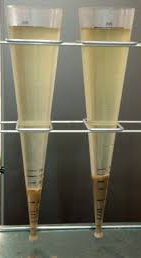
\includegraphics[scale=0.7]{ImhoffCone}\\
%			      		Imhoff Cone\\
%			      		\emph{Note the ml marking at the bottom of the cone}
%			      	\end{center}
%			      \end{minipage}
%			\item One factor which affects settleability is the conveyance time of the sewage to the treatment plant. 
%			\item The settleable component of the suspended solids will decrease as the sewage becomes more septic due to longer conveyance times.
%			\item Influent and effluent total suspended solids are measured to establish the overall treatment and individual process efficiencies.  
%			\item Volatile solids measurements before and after biological processes such as secondary treatment and digestion provide information on the process efficiency.\\
%		\end{itemize}
%		\begin{enumerate}%$$$$$$$$$$$$$$$$$$$$%
%			\definecolor{shadecolor}{RGB}{220, 220, 220}
%			\begin{snugshade*}
%				\item \noindent\textsc{Procedures for Solids Analysis}
%			\end{snugshade*}		
%			
%			\begin{enumerate}[a.]
%				\definecolor{shadecolor}{RGB}{110, 192, 221}
%				\begin{snugshade*}
%					\item \noindent\textsc{Determining wastewater suspended solids - Total(TSS) and Volatile(VSS) concentrations:}
%				\end{snugshade*}
%				 
%				%\hl{How total suspended solids concentration is established for a wastewater sample:}
%				\begin{itemize}
%					\item A known volume of wastewater sample is filtered through a pre-weighed filter paper
%					\item The suspended solids will be retained by the filter
%					\item The water with the dissolved solids will pass through the filter
%					\item The filter paper with the filter solids is rinsed with distilled water to remove 
%					\item The filter paper with the solids is dried in the oven and then weighed
%					\item The difference between the weight of the dried filter paper with the solids and the pre-weighed filter paper, measured in mg, will be the suspended solids in: mg per the original quantity of wastewater sample taken.  This value can be converted to give the suspended solids content in mg/l
%					\item A filter paper with the dried solids is incinerated in a muffler furnace
%					\item The difference in the weight of the solids, before and after incineration is the fixed solids
%					\item The difference between the weight of the solids before incineration and the fixed solids is the volatile solids
%				\end{itemize}
%				
%				
%				
%				\begin{snugshade*}
%					\item \noindent\textsc{Determining wastewater and sludge total solids (TS) and volatile solids (VS) concentrations:}
%				\end{snugshade*}
%				\begin{itemize}
%					\item A certain quantity of wastewater (by volume) or sludge (by weight) is taken in a pre-weighed dish and weighed.  Note:  the sample is not filtered.
%					\item The dish with the sample is dried in an oven
%					\item The difference in the weight of the pre-weighed dish from that of the dish with the dried sample is the total solids
%					\item The dried solids are incinerated in a muffler furnace
%					\item The difference in the weight of the solids, before and after incineration is the fixed solids
%					\item The difference between the fixed solids and the total solids is the volatile solids
%					\item Total solids of a sludge sample is reported as a \% of the sludge weight.  A 7\% sludge has 7 lbs of solids for every 100 lbs of sludge.
%				\end{itemize}
%				
%							
%				
%				
%					\hl{For sludge samples, volatile solids is typically reported as the volatile solids fraction in \% of the total solids content of the sludge.  For example, if a 8\% sludge (i.e sludge which has 8\% TS or 80,000mg/l solids), is reported to have 70\% volatile, it means that 70\% of the total solids - 0.7*8\%=5.6\% or 56,000mg/l is the sludge volatile solids content.  \emph{70\% volatile does not meet the sludge has 700,000mg/l volatile solids}}\\
%				
%			\end{enumerate}
%			
%			\begin{snugshade*}
%				\item \noindent\textsc{Summary of Wastewater Solids}
%			\end{snugshade*}
%			\begin{itemize}
%				\item Solids in wastewater can be categorized as dissolved or suspended
%				      \begin{itemize}
%				      	\item Suspended solids can be further categorized as settleable or unsettleable
%				      \end{itemize}
%				\item Solids can also be categorized as organic (aka: volatile) or inorganic (aka: fixed)
%				\item Colloidial particles are small sized particles some of which pass through the filter and accounted as part of dissolved solids
%				\item TSS - Total Suspended Solids are the solids that are captured on the filter paper upon filtration of the wastewater sample.  
%				\item Wastewater samples typically analyzed for TSS include:  plant, primary and secondary processes - influent and effluent.  TSS is reported in mg/l
%				\item TS - Total Solids are solids content of sludge.  TS of sludge is established by drying a preweighed quantity of sludge in an oven and is typically reported as \% solids - which is how many parts (by weight) of solids per 100 parts (by weight) of sludge.
%				\item Volatile solids are solids that are removed when the solids are incinerated at 550°C.  The solids that remain after incineration are fixed or non-volatile or inorganic solids.
%			\end{itemize}
%			
%			\begin{snugshade*}
%				\item \noindent\textsc{Typical influent wastewater contains:}
%			\end{snugshade*}
%			\begin{itemize}
%				\item Less than 0.1\% total solids.  Total solids concentration in typical wastewater is about 750mg/l
%				\item The total solids are 50\% organic (volatile) and 50\% inorganic (fixed)
%				\item Of the total solids, dissolved solids constitute about 70\% of the solids and the remaining 30\% solids are suspended solids
%				\item 40\% of the dissolved solids are volatile the remaining 60\% are fixed
%				\item 70\% of the suspended solids are volatile and the remaining 30\% are fixed
%			\end{itemize}
%			\newpage
%			\begin{sidewaysfigure}
%				\begin{center}
%					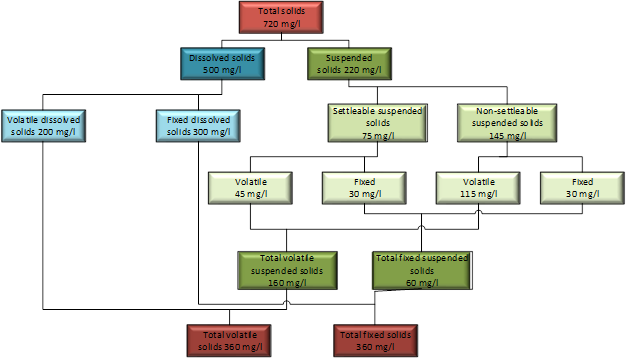
\includegraphics[scale=1.1]{WastewaterSolids}\\
%					Typical Wastewater Solids Concentrations
%				\end{center}
%			\end{sidewaysfigure}
%			\pagebreak
%			\end{enumerate}
%				
%			
%			\begin{snugshade*}
%				\item \noindent\textsc{Nutrients}
%			\end{snugshade*}	
%			\begin{itemize}
%				\item Plant nutrients - nitrogen and phosphorous, present in wastewater effluent discharge, promote growth of plant and algal matter in the receiving waters causing destruction of the normal aquatic life mainly due to oxygen depletion - eutrophication.
%				      
%				\item Because of the potential impacts of the presence of these nutrients in wastewater effluent on the receiving waters,  limits on the levels of these nutrients is typically stipulated in the treatment plant's wastewater discharge permit.
%				      
%				\item Typically, conventional secondary treatment processes are designed primarily remove the organics from the wastewater.  Secondary treatment process designed to additionally remove nutrients is deemed as tertiary or advanced treatment is termed as Biological Nutrient Removal (BNR).
%			\end{itemize}
%			
%			\begin{enumerate}%@@@@@@@@@@@@@@@@@@%
%				\definecolor{shadecolor}{RGB}{220,220,220}
%				\begin{snugshade*}
%					\item \noindent\textsc{Nitrogen}%@@@@@@@@@@@@@@@@@@%
%				\end{snugshade*}
%				\begin{itemize}
%					\item Forms of nitrogen:\\
%					      \begin{itemize}
%					      	\item About 60\% of nitrogen in wastewater is present as ammonia nitrogen (about 60\%).  The ammonium nitrogen is present either in the form of ammonia (NH$_3$ ) or as ammonium (NH$_4^+$ ) ion.   These two forms can rapidly change from one to the other depending on pH and temperature.  Under low pH (acidic) or neutral conditions – pH less than or equal to 7, ammonia exists mostly as ammonium.  Ammonia becomes the dominant form as the pH increases to 8 and beyond.
%					      	\item The other dominant form of nitrogen, about 40\% of the total nitrogen is as organic nitrogen
%					      	\item Nitrogen measured as Total Kjeldahl Nitrogen (TKN) which is the sum of the organic nitrogen and the ammonia nitrogen concentrations.  Total inorganic nitrogen is the total concentration of ammonia nitrogen, NO3-, and NO2-.   Table provides the concentrations and forms of nitrogen in wastewater.
%					      \end{itemize}
%					      \setlength{\arrayrulewidth}{0.7mm}
%					      \setlength{\tabcolsep}{8 pt}
%					      \renewcommand{\arraystretch}{0.8}
%					      \begin{center}
%					      	\noindent \begin{tabular}{ |p{6cm}|p{2.0cm}|p{2.5cm}|p{2.cm}|}
%					      	\hline
%					      	\multicolumn{4}{|c|}{\textbf{Forms of Nitrogen in Wastewater}} \\
%					      	\hline
%					      	%\thead{A Head} & \thead{A Second \\ Head} & \thead{A Third \\ Head} \\
%					      	%\hline%
%					      	
%					      	\hspace{1.8 cm}Forms of Nitrogen & \hspace{0.25 cm} Formula & \hspace{.4 cm} Found in & \hspace{.4 cm} Typical \newline \hspace{.2 cm}Concentration\\
%					      	\hline
%					      	\small Ammonia/Ammonium & \small NH$_3$/NH$_4^{\enspace +}$ &  \small Influent wastewater & 30-50 mg/l\\
%					      	
%					      	Total Kjeldahl Nitrogen \newline  \small (Ammonia/Ammonium + Organic Nitrogen) &  \small TKN &  \small Wastewater \newline  \small effluent  & 30-60 mg/l \\
%					      	
%					      	\small Total Inorganic Nitrogen \newline  \small (Ammonia/Ammonium + Nitrite + Nitrate) & \small TIN &  \small  Wastewater \newline  \small effluent  & 1-40 mg/l \\
%					      	
%					      	\small Nitrate  & $NO_3^{\enspace -}$ &  \small Nitrified effluent &  \small 1-35 mg/l \\
%					      	
%					      	\small Nitrate  &  $NO_2^{\enspace -}$ &  \small Partially nitrified effluent &  \small 0.1-2 mg/l \\
%					      	
%					      	\hline
%					      	\end{tabular}
%					      	
%					      \end{center}
%					      
%					      The nitrogen cycle which shows how nitrogen is converted into its various chemical forms is shown below.
%					      
%					\item Nitrogen removal as part of the secondary treatment mainly involves nitrification-denitrification processes which involve conversion of ammonia nitrogen to nitrogen gas.
%					      
%				\end{itemize}
%				\begin{snugshade*}
%					\item \noindent\textsc{Phosphorous}
%				\end{snugshade*}
%				\begin{itemize}
%					
%		
%		
%		
%	
%	
%	
%	%
%	%\begin{enumerate}
%	%	\definecolor{shadecolor}{RGB}{179, 203, 203}
%	%\begin{snugshade*}
%	%\item \noindent\textsc{Solids Analysis}%$$$$$$$$$$$$$$$$$$$$%
%	%\end{snugshade*}
%	%
%	%\vspace{0.4cm}
%	%\end{enumerate}
%	%\begin{snugshade*}
%	%\item \noindent\textsc{BOD}%$$$$$$$$$$$$$$$$$$$$%
%	%\end{snugshade*}
%	
%	
%\end{enumerate}



\part{Week 3}
% \documentclass{article}
% %\usepackage[english]{babel}%
% \usepackage{graphicx}
% \usepackage{tabulary}
% \usepackage{tabularx}
% \usepackage[normalem]{ulem}
% \usepackage{cancel}
% \usepackage{tikz} 
% \usepackage{pdflscape}
% \usepackage{colortbl}
% \usepackage{lastpage}
% \usepackage{multirow}
% \usepackage{enumerate}
% \usepackage[shortlabels]{enumitem}
% \usepackage{color,soul}
% \usepackage{pdflscape}
% \usepackage{hyperref}
% %\usepackage[table]{xcolor}
% \usepackage{rotating}
% \usepackage{amsmath}
% \usepackage{fixltx2e}
% \usepackage{framed}
% \usepackage{mdframed}
% \usepackage[T1]{fontenc}
% \usepackage[utf8]{inputenc}
% \usepackage{textcomp}
% \usepackage{siunitx}
% \usepackage{ifthen}
% \usepackage{fancyhdr}
% \usepackage{gensymb}
% \usepackage{newunicodechar}
% \usepackage[document]{ragged2e}
% \usepackage[margin=1in,top=1.1in,headheight=57pt,headsep=0.1in]
% {geometry}
% \usepackage{ifthen}
% \usepackage{fancyhdr}
% \everymath{\displaystyle}
% \usepackage[document]{ragged2e}
% \usepackage{fancyhdr}
% \everymath{\displaystyle}
% \usepackage{empheq}

% \usepackage[most]{tcolorbox}

% \usepackage{booktabs} % Required for nicer horizontal rules in tables


% \usepackage{enumitem}

% %\usepackage[table,xcdraw]{xcolor}
% \usetikzlibrary{arrows}
% \linespread{2}%controls the spacing between lines. Bigger fractions means crowded lines%
% %\pagestyle{fancy}
% %\usepackage[margin=1 in, top=1in, includefoot]{geometry}
% %\everymath{\displaystyle}
% \linespread{1.3}%controls the spacing between lines. Bigger fractions means crowded lines%
% %\pagestyle{fancy}
% \pagestyle{fancy}
% \setlength{\headheight}{56.2pt}

% \definecolor{myblue}{rgb}{.8, .8, 1}
% \newcommand*\mybluebox[1]{%
% \colorbox{myblue}{\hspace{1em}#1\hspace{1em}}}

% \chead{\ifthenelse{\value{page}=1}{
\includegraphics[scale=0.3]{SCC}\\ \textbf \textbf Wastewater Constituents Analysis \& Laboratory Methods}}
% \rhead{\ifthenelse{\value{page}=1}{}{}}
% \lhead{\ifthenelse{\value{page}=1}{}{Wastewater Constituents Analysis \& Laboratory Methods}}
% \rfoot{\ifthenelse{\value{page}=1}{Module 1: WATR 048 - Spring 2019}{Module 1: WATR 048 - Spring 2019}}

% \lfoot{Shabbir Basrai}
% \cfoot{Page \thepage\ of \pageref{LastPage}}
% \renewcommand{\headrulewidth}{2pt}
% \renewcommand{\footrulewidth}{1pt}
% \begin{document}
% %\begin{empheq}[box=\mybluebox]{align}
% %a&=b\\
% %E&=mc^2 + \int_a^a x\, dx
% %\end{empheq}

% \newlist{steps}{enumerate}{1} % Defines "Steps" for enumerate as Step 1, Step 2 etc.
% \setlist[steps, 1]{label = Step \arabic*:} % Defines "Steps" for enumerate as Step 1, Step 2 etc.

% \setlist{nolistsep} % Reduce spacing between bullet points and numbered lists


%_______________________________________________________________________________________________________________________________________%
\chapterimage{Preliminary.jpg} % Chapter heading image

\chapter{Preliminary Treatment}
% \begin{enumerate}[1.]
% 	\definecolor{shadecolor}{RGB}{200, 200, 240}

% 	%%%%%%%%%%%
% 	% LEVEL 2 %
% 	%%%%%%%%%%%

% 	\begin{snugshade*}
% 		\item \noindent\textsc{Wastewater Constituents}%$$$$$$$$$$$$$$$$$$$$%
% 	\end{snugshade*}
% 	Solids, organic matter, nutrients, pathogens and oil \& grease are the main target constituents of wastewater treatment operations.
% 	\begin{enumerate}[A.]%___________%
% 			\definecolor{shadecolor}{RGB}{225, 235, 235}

				%%%%%%%%%%%
				% LEVEL 3 %
				%%%%%%%%%%%
		% \begin{snugshade*}
		% 	\item \noindent\textsc{Organic Matter}%###############################%
		% \end{snugshade*}






			\begin{itemize}
				\item The objective of preliminary treatment is to remove coarse solids and other large materials often found in raw wastewater
				\item Removal of these materials is necessary to enhance the operation and maintenance of subsequent treatment units\\
				\item Preliminary treatment operations typically include a combination of the following processes:
					\begin{itemize}
						\item Screening
						\item Grinding or shredding
						\item Flow measurement
						\item Grit removal
						\item Pre-aeration
						\item Flow equalization
					\end{itemize}
			\end{itemize}

				
		\section{Process Elements of Preliminary Treatment}\index{Process Elements of Preliminary Treatment}	
			
		\subsection{Screening}\index{Screening}
					\begin{itemize}
						\item Screening is typically the first unit in a preliminary treatment
						\item Screening allows for the capture of coarse solids as pieces of cloths garbage so as to protect pumps and other units from clogging. 
						\item Screens may consist of vertical or inclined bars (bar racks or bar screens), wire mesh or perforated plates having either circular or rectangular openings. 
						\item Screens remove the large, entrained, suspended or floating solids such as pieces of wood, cloth, paper, plastics, garbage, etc.
						\item Debris collected on the screen can be cleaned manually or automatically using chain driven rakes 
						\item The retained material at screens - screenings, is collected and hauled to landfill for disposal
						\item The quantity of screenings removed varies by location and is a function of the clear opening of the screen.
						\item Barmuinitors combine the function of a screen and a grinder.  The ground material is returned to the wastewater flow for removal during primary treatment.
					\end{itemize}

\begin{figure}
\begin{center}
    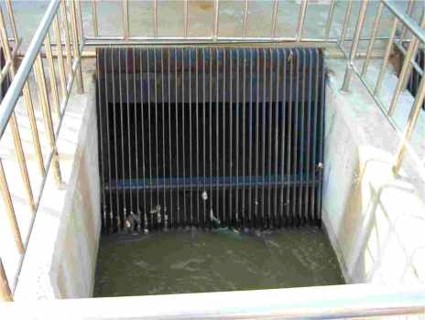
\includegraphics[width=0.7\linewidth]{Barscreen}\\

Barscreen - No rakes
\end{center}
  \end{figure}
  
 \begin{center}
    
\includegraphics[scale=0.6]{Blank}\\
\hspace{0cm} Video: Automatic Barscreen
  \end{center}
 
		\subsection{Grinding and Shredding}\index{Grinding and Shredding}

					\begin{itemize}
\begin{minipage}{\textwidth}	\item Comminutor(Grinder) consist of fixed, rotating or oscillating teeth or blades, acting together to reduce the solids to a size which will pass through fixed or rotating screens grind rags into small chunks
\item The comminutors are installed in wastewater channel and they grind the larger solids without actually removing them from the wastewater.  These devices may be installed before the screens or as a combination of screen and cutters (barmunitors).
					\end{minipage}	
					\end{itemize}
					\begin{minipage}{\textwidth}
					\begin{center}
      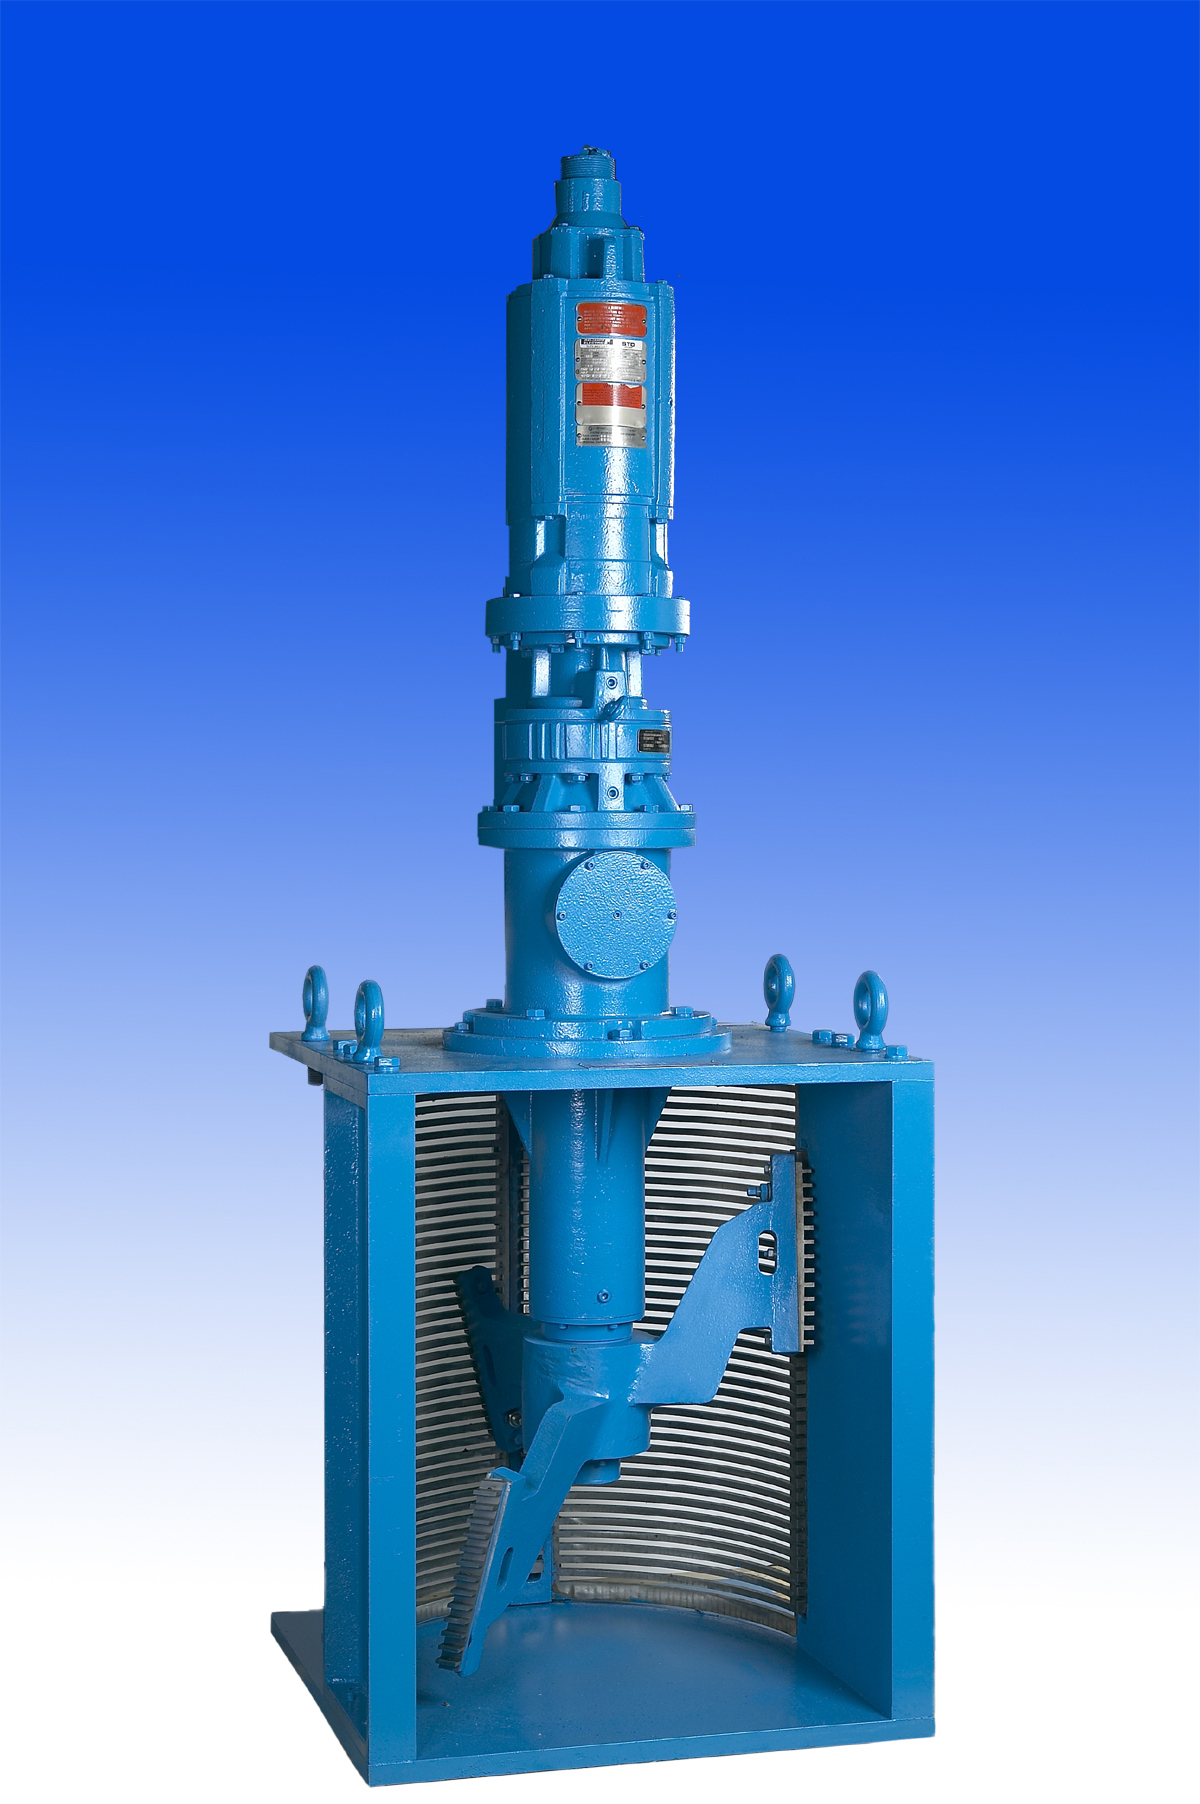
\includegraphics[width=0.3\linewidth, height=70mm]{Comminutor}\\
      Comminutor\\
\end{center}
    \end{minipage}

\begin{figure}[h]
    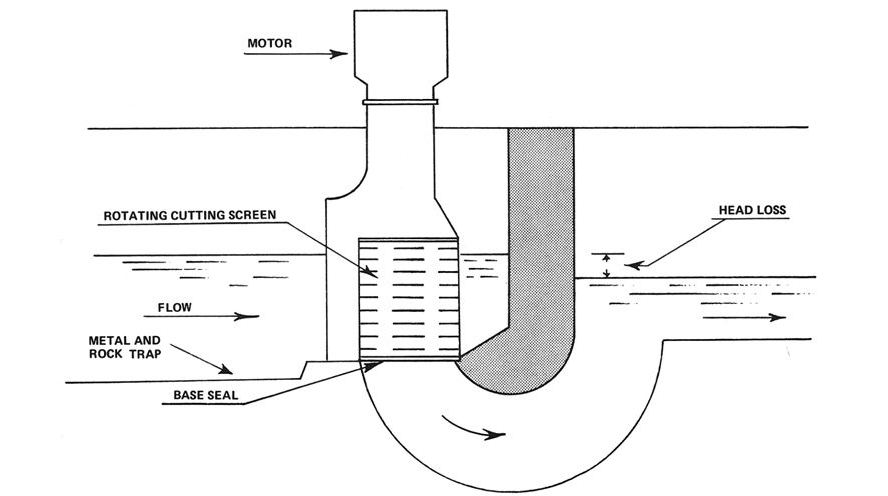
\includegraphics[width=\linewidth]{Comminutor1}\\
    \hspace{5cm}Schematic of comminutor placement in a channel\\
%    \caption{Comminutor Schematic}
  \end{figure}
  
		\subsection{Flow Measurement}\index{Flow Measurement}
					\begin{itemize}
						\item Wastewater flow to a treatment plant is not constant but varies in a diurnal (daily) pattern reflecting domestic water use activity.
						\item Continuous flow measurement is necessary in order to monitor diurnal variations in flow which may affect treatment plant efficiency.\\
						\item Devices used for flow measurement as part of the preliminary treatment can be placed in a channel or in a pipe.
					\end{itemize}

		\subsubsection{Devices for Flow Measurement in Channels}\index{Devices for Flow Measurement in Channels}

					\begin{itemize}
						\item Weirs: 
							\begin{itemize}
								\item Typically sharp crested weirs which are essentially metal plates installed perpendicular the flow.  The plate may a straight edge, a V-notch, or a trapezoidal opening.
								\item The weir plate in the channel causes an increase in the depth of the water behind the weir.  which is proportional to the flow rate.
								\item The flow rate can be determined by calculation or by reading the corresponding flow value to the depth of the water, from a chart specific for that weir. 
								
						
\begin{figure}[h!]
  \centering
  \begin{subfigure}[b]{0.4\linewidth}
    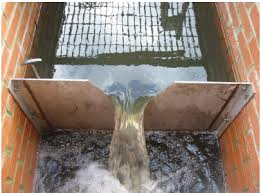
\includegraphics[width=\linewidth]{ChannelWeir}
    \caption{Weir in a channel}
  \end{subfigure}
  \hspace{1cm}
  \begin{subfigure}[b]{0.4\linewidth}
    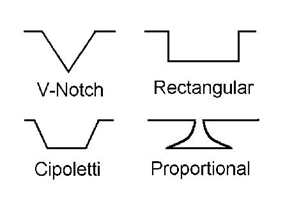
\includegraphics[width=\linewidth]{WierTypes}
    \caption{Weir types}
  \end{subfigure}
\end{figure}
								
								
								
							\end{itemize}
						\item Parshall Flume:
							\begin{itemize}
								\item Parshall flume uses a narrow section in the channel as the restriction rather than the vertical plate of a weir.
								\item Like the weir, the restriction due to the narrow section of the flume, causes an increase in the depth of the water behind the weir (head) which is proportional to the flow rate.
								\item The flow rate can be determined by calculation or by reading the corresponding flow value to the depth of the water, from a chart specific for that Parshall Flume. 
								\end{itemize}

					\end{itemize}
\begin{figure}[h!]
  \centering
  \begin{subfigure}[b]{0.4\linewidth}
    \includegraphics[width=0.75\linewidth]{parshallflume1}
    \caption{Parshall flume}
  \end{subfigure}
  \hspace{1cm}
  \begin{subfigure}[b]{0.4\linewidth}
    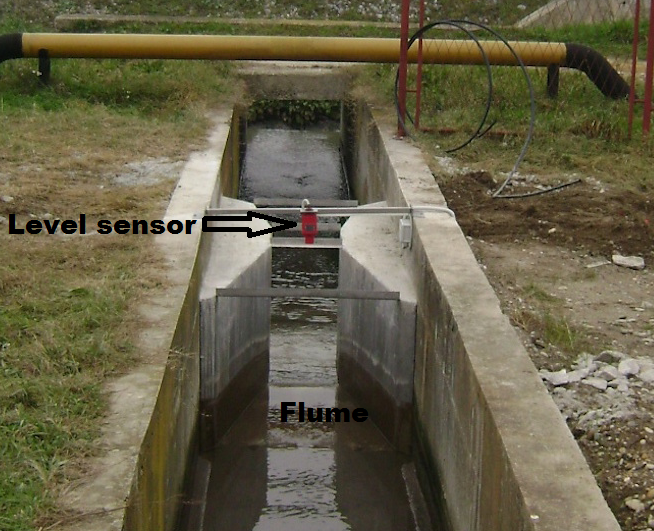
\includegraphics[width=\linewidth]{parshallflume2}
    \caption{Parshall flume with level sensor}
  \end{subfigure}
\end{figure}
		\subsubsection{Devices for Flow Measurement in Pipes}\index{Devices for Flow Measurement in Pipes}
					
					\begin{itemize}
						\item Venturi Tube:
							\begin{itemize}
								\item Measures the difference in pressure in the inlet and center section (throat)
								\item This pressure difference can then be mathematically converted to a flow rate.
								\item Works only when a pipe if flowing full
							\end{itemize}
						\item Magnetic Flow Meter (Magmeter):
							\begin{itemize}
								\item Magmeter is a pipe spool which has an electromagnetic coil surrounding it.  As the wastewater - a conducting material, flows through it, an electrical current is created proportional to the velocity of the conducting fluid (wastewater).
								\item Flow is automatically calculated by multiplying the velocity by the cross- sectional area of the pipe.
								\item Similar to the venturi meter, magmeter will read accurately only if the magmeter section of the pipe is flowing full and the wastewater is flowing through it at a certain minimum velocity.
							\end{itemize}
\begin{figure}[h!]
  \centering
  \begin{subfigure}[b]{0.4\linewidth}
    \includegraphics[width=0.9\linewidth]{magmeter1}
    \caption{Magmeter}
  \end{subfigure}
  \hspace{1cm}
  \begin{subfigure}[b]{0.45\linewidth}
    \includegraphics[width=\linewidth]{magmeter}
    \caption{Piping with magmeters}
  \end{subfigure}
\end{figure} 
					\end{itemize}
		\subsection{Grit Removal}\index{Grit Removal}
						\begin{itemize}
							\item Grit includes sand, gravel, cinder, eggshells, bone chips, seeds, coffee grounds, and large organic particles, such as food waste.
							\item Purpose of Grit removal:
								\begin{itemize} 
									\item to protect mechanical equipment from abrasion and abnormal wear 
									\item to reduce clogging caused by deposition of grit particles in pipes and channels, and 
				\item to prevent loading the treatment plant with inert matter that might interfere with the operation of treatment units such as anaerobic digester and aeration tanks.
			\end{itemize}
		\item Removal of organic material along with the grit is undesirable for two reasons:
			\begin{enumerate}
				\item It causes odor issues, and 
				\item Organic matter is a potential source of energy (digester gas)
			\end{enumerate}
		\item Grit Disposal: Grit removed is typically landfilled.
		\item Grit Volume:  The volume of grit collected measured in ft$^3$/MG.
		\item The rate of grit collection can range from 0.5 ft$^3$/MG to 30 ft$^3$/MG.
		\item Wastewater plants having a combined collection system must deal with much larger volumes of grit.
\end{itemize}
\subsubsection{Grit Removal Systems}\index{Grit Removal Systems}



			\begin{itemize}
			
					\item \noindent\textsc{Horizontal grit chambers:}

					\begin{itemize}
						\item These are rectangular channels 30 to 60 feet long and the water detention time is between 45 to 90 seconds
						\item Water passing through these channels is maintained at a relatively constant \hl{velocity of about 1 feet per second (fps)} which allows for the grit to settle while keeping the lighter organic material to stay in suspension and continue on into the primary clarifiers.
					\end{itemize}
	

						\item \noindent\textsc{Aerated grit chambers:}
	
					\begin{itemize}
						\item The 1 fps velocity is maintained by using aerators to create a rolling flow in the tank.
						\item Aeration is achieved using diffusers located on the bottom of one side of the grit chamber.
						\item Aerated grit chambers help create aerobic conditions in septic sewage. Aerobic conditions help improve the settleability of the sludge and increase both BOD and suspended solids removal in the primary clarifiers.
						\item Much larger and deeper than non-aerated units.
						\item The detention times are increased to 3 to 5 minutes.
					\end{itemize}

\begin{figure}[h!]
  \centering
  \begin{subfigure}[b]{0.46\linewidth}
    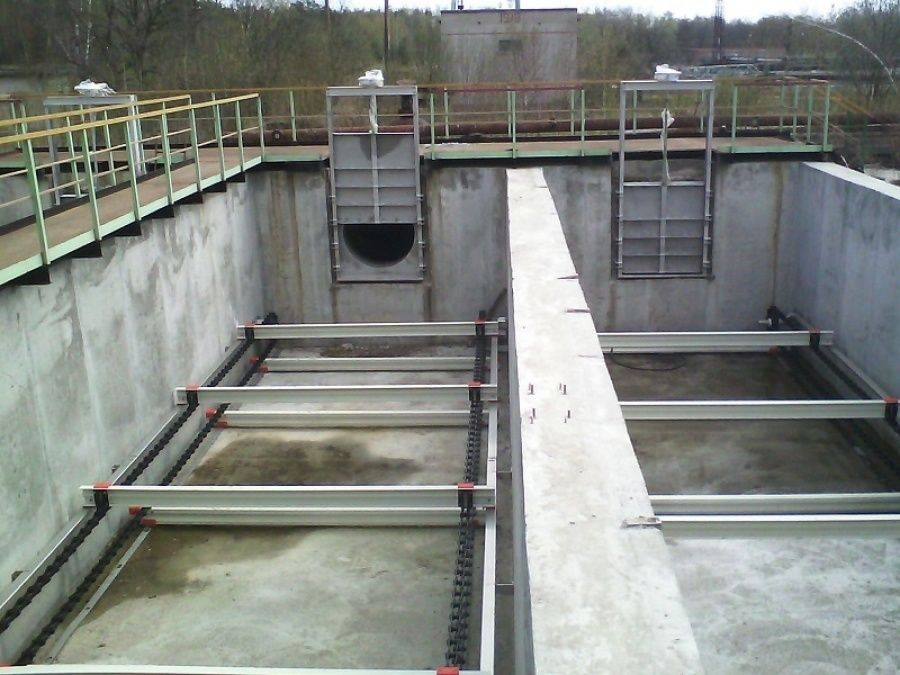
\includegraphics[width=0.8\linewidth]{HorizontalGritChamber}
    \caption{Horizontal grit chamber}
  \end{subfigure}
  \hspace{0.2cm}
  \begin{subfigure}[b]{0.5\linewidth}
    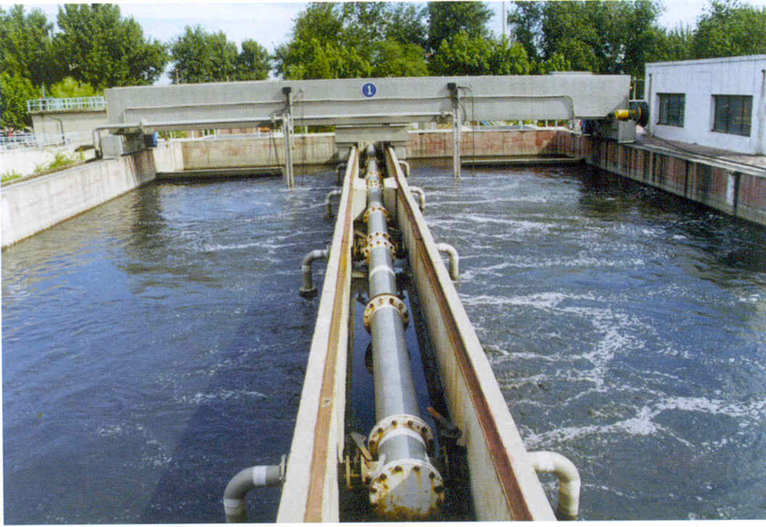
\includegraphics[width=0.8\linewidth]{AeratedGritChamber}
    \caption{Aerated grit chamber}
  \end{subfigure}
\end{figure} 					


						\item \noindent\textsc{Cyclonic/Vortex grit chamber:}


					\begin{itemize}
						\item The wastewater flows into a cylinder that tapers to a cone at one end.
						\item The flow whirls around the inside of the cylinder like a cyclone which causes the heavy grit to be slinged to the outside and it ultimately settles to the bottom from where it is withdrawn.
					\end{itemize}

\begin{figure}[h!]
  \centering
  \begin{subfigure}[b]{0.47\linewidth}
    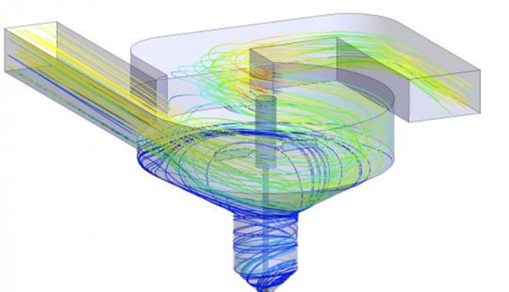
\includegraphics[width=0.8\linewidth]{VortexGritChamber1}
    \caption{Vortex grit chamber design}
  \end{subfigure}
  \hspace{0.2cm}
  \begin{subfigure}[b]{0.43\linewidth}
    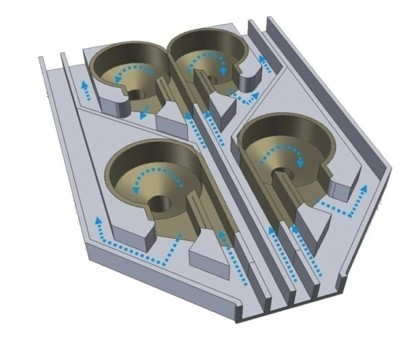
\includegraphics[width=0.8\linewidth]{VortexGritChamber}
    \caption{Vortex grit chamber installed}
  \end{subfigure}
\end{figure} 
	
\subsubsection{Grit Removal}\index{Grit Removal}		

		
			\begin{itemize}
				\item In the cyclonic/vortex grit chamber, the grit is scoured with water and is removed using pumps
				\item For the horizontal and aerated grit systems:
					\begin{itemize}
						\item Mechanical augers at the bottom of the grit chamber move the grit to one end of the tank where grit slurry pumps can pump it out of the tank to a grit separator.
						\item In some cases steep bottom slope is provided which will collect the grit at Central Point of Removal.
						\item Grit Removal is achieved by air pumps for small aerated grit chambers.
						\item Grit can also be removed by tubular conveyors, buckets type collectors, elevators screws conveyors, grit pumps and clam shell buckets
					\end{itemize}
			\end{itemize}
						\end{itemize}
%		\end{itemize}

\subsection{Flow Control}\index{Flow Control}	
	\begin{itemize} 
		\item Flow control is critical for grit removal, specifically for the horizontal and aerated grit chambers as excessive or inadequate velocities would lead to poor grit removal or cause excessive organic material settling along with the grit, respectively
		\item As the wastewater flows vary diurnally, it is important that velocity of the wastewater in the grit chamber should be maintained nearly constant - near 1 fps.
		
\begin{figure}[h]
    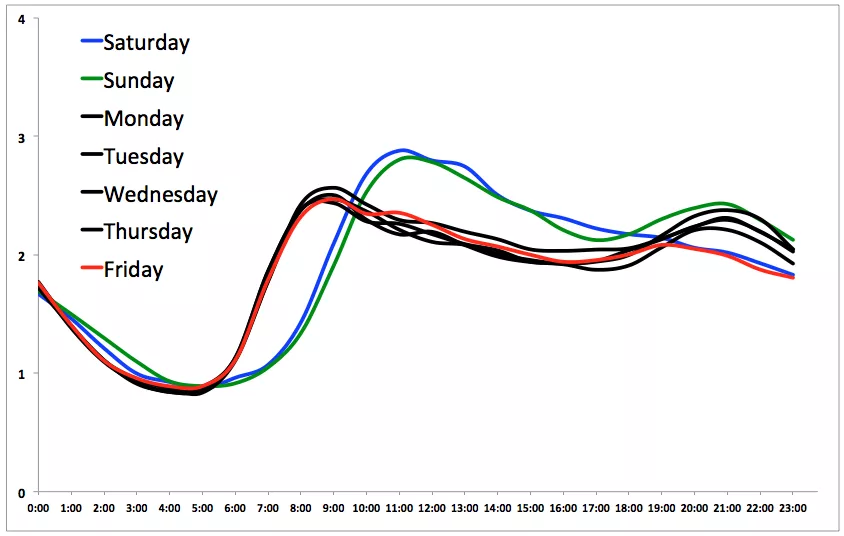
\includegraphics[width=\linewidth]{DiurnalFlow}\\
\begin{center}
Diurnal wastewater flow profile \\
\end{center}
%    \caption{Comminutor Schematic}
  \end{figure}		

		\item Constant velocity in a grit chamber is achieved by providing a \hl{proportional (Sutro) weir} at the outlet end of grit chamber.
		\item The shape of the opening between the plates of a proportional weir is made in such a way that the discharge is directly proportional to liquid depth in grit chamber resulting in maintaining a constant velocity of water even a the flow changes.
	\end{itemize}
\begin{figure}[h!]
  \centering
  \begin{subfigure}[b]{0.5\linewidth}
    \includegraphics[width=0.8\linewidth]{Sutroweir1}
    \caption{Proportional weir design}
  \end{subfigure}
  \hspace{1cm}
  \begin{subfigure}[b]{0.35\linewidth}
    \includegraphics[width=0.8\linewidth]{Sutroweir}
    \caption{Installed Proportional weir}
  \end{subfigure}
\end{figure} 

\subsection{Pre-aeration}\index{Pre-aeration}	
	\begin{itemize}
		\item Pre-aeration of the wastewater as part of the preliminary treatment may be provided as a separate process or increased detention time in an aerated grit chamber.
		\item Pre-aeration provides the follwoing benefits:
			\begin{itemize}
				\item freshens up wastewater by dissolving oxygen thereby reducing the wastewater septicity
				\item reduction of septicity allows for better settling - solids and BOD removal, in the following primary treatment process
				\item promotes grease separation which facilitates its removal during primary treatment
			\end{itemize}
	\end{itemize}
\subsection{Flow Equalization}\index{Flow Equalization}	

	\begin{itemize}
		\item Flow equalization involves storing a portion of peak flows for release during low-flow periods
		\item It prevents surges and allows for the operation of processes at design flows thus allowing for optimal physical, biological and chemical processes to take place.
		\item It results in saving capital costs as the processes may be built with a treatment capacity which is less than the peak flows
	\end{itemize}

\section{Preliminary Treatment Math Problems}\index{Preliminary Treatment Math Problems}

Preliminary Treatment math problems relate to the following:

\subsection{Channel Velocity and Flow Rate}\index{Channel Velocity and Flow Rate}
Flow Rate - Q (volume/time) = velocity (distance or length traveled /time) * surface area\\
Velocity is the speed at which the water is flowing.  It is measured in units of length/time – ft./sec.\\
Velocity of water flowing through can be calculated by dividing the flow rate by area of the flow stream.\\
\vspace{0.5cm}
$Velocity \enspace \dfrac{length}{time}= \dfrac{flow \enspace rate(\dfrac{volume \enspace or \enspace cubic \enspace length}{time})}{surface \enspace area \enspace in \enspace the \enspace direction \enspace of \enspace flow-square \enspace length}$\\
\vspace{0.5cm}
\textbf{For a flow in a channel:}\\
\vspace{0.5cm}
\hl{Example Problems:}\\
\begin{enumerate}[1.]
\item Calculate the velocity of a 14 MGD flow in a 6 ft wide channel with a water depth of two feet.\\
\begin{center}
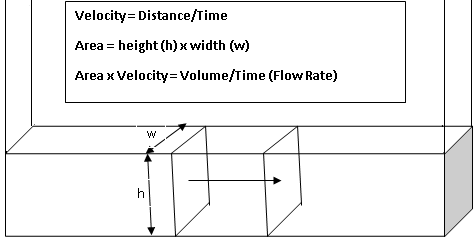
\includegraphics[scale=0.5]{ChannelFlow3}
\end{center}
$Flow (Q) = Velocity (V) * Area (A)$\\
$\implies 14 \dfrac{MG}{day}* \dfrac{10^6 gal}{MG} * \dfrac{ft^3}{7.48 gal}*\dfrac{day}{24*60*60} = V \dfrac{ft}{sec}* 6 ft * 2 ft \implies 21.7 \dfrac{ft^3}{sec}= 12V\dfrac{ft^3}{sec}$\\
$\implies V \dfrac{ft}{sec}= \dfrac{21.7}{12}= \boxed{1.8\dfrac{ft}{sec}}$\\

\item Calculate the flow, in gpd, that would pass through a grit chamber 2 feet wide, at a depth of 6 inches, with a velocity of 1 ft /sec\\
Solution:\\
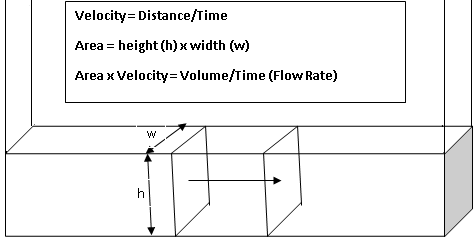
\includegraphics[scale=0.5]{ChannelFlow3}\\
$Q=V*A$\\
$Q=1\dfrac{ft}{s}*(2*0.5)ft^2=1\dfrac{ft^3}{s}$\\
$Q=1\dfrac{\cancel{ft^3}}{\cancel{s}}*\dfrac{(1440*60)\cancel{s}}{day}*7.48\dfrac{gal}{\cancel{ft^3}}=\boxed{646,272\dfrac{gal}{day}}$
\vspace{0.5cm}
\item A wastewater channel is 3.25 feet wide and is conveying a wastewater flow of 3.5 MGD. The wastewater flow is 8 inches deep. Calculate the velocity of this flow.\\
Solution:\\
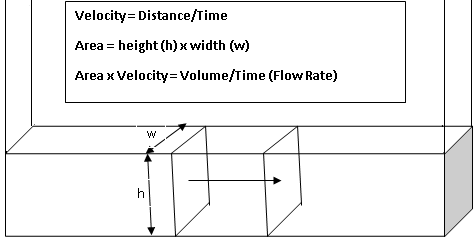
\includegraphics[scale=0.5]{ChannelFlow3}\\
$Q=V*A \implies V=\dfrac{Q}{A}$\\
$\implies V\dfrac{ft}{s}=\dfrac{3.5\dfrac{\cancel{MG}}{\cancel{day}}*\dfrac{1000000\cancel{gal}}{\cancel{MG}}*\dfrac{ft^{\cancel{3}}}{7.48\cancel{gal}}*\dfrac{\cancel{day}}{(1440*60)s}}{(3.25*0.75)\cancel{ft^2}}=\boxed{2.2\dfrac{ft}{s}}$
\vspace{0.5cm}
\item A plastic float is dropped into a wastewater channel and is found to travel 10 feet in 4.2 seconds. The channel is 2.4 feet wide and is flowing 1.8 feet deep. Calculate the flow rate of this wastewater in cubic feet per second.\\
Solution:\\
$Q=V*A$\\
$\implies Q\Big(\dfrac{ft^3}{s}\Big)=\dfrac{10ft}{4.2s}*(2.4*1.8)ft^2=\boxed{10.3\dfrac{ft^3}{s}}$
\end{enumerate}

\subsection{Grit Removal Rates}\index{Grit Removal Rates}
\emph{Typical grit removal ranges from 0.5 to 30 ft$^3$/MG}\\
\vspace{0.3cm}
\hl{Example Problems:}\\
\begin{enumerate}[1.]
\item At a wastewater treatment plant which receives a flow rate of 650,000 gallons per day, a total of 50 cubic feet of grit was removed for the month. Calculate the rate of grit removal assuming 30 days in a month.\\
Solution:\\
$Grit Removal\dfrac{ft^3}{MG}=50\dfrac{ft^3}{ \cancel{month}}*\dfrac{\cancel{month}}{30\cancel{days}}*\dfrac{\cancel{day}}{650,000\cancel{gal}}*1,000,000\dfrac{\cancel{gal}}{MG}=\boxed{2.6\dfrac{ft^3}{MG}}$
\end{enumerate}
%----------------------------------------------------------------------------------------------%
\chapterimage{Week3Clarifier1.jpg} % Chapter heading image

\chapter{Primary Treatment}

%\section{Background}\index{Background}
\begin{itemize}
\item Synonyms:  primary treatment basin, primary clarifier, sedimentation basin, primaries, clarifier

	
		\item Primary treatment is after preliminary treatment and 				before secondary treatment
		\item Its two main objectives are: 
			\begin{itemize}
				\item Remove settleable solids
				\item Remove floatable solids
			\end{itemize}
		\item This is a physical process which relies on the physical 			properties - how heavy or light the suspended solids particles 		are to effect its separation
		\item Provides quiescent conditions for the influent 					wastewater for the heavier solids to settle and the lighter 			solids to float
		\item Removes settleable solids and floatables
		\item Settled solids are removed as sludge from the bottom of 			the clarifier
		\item Floatable solids including oil and grease are also 				removed, as scum from the surface\\
		\item The shape of the primary clarifier is either rectangular 		or circular
	
		\item Effective solids removal in the primary clarifiers will 			reduce the loading on the expensive secondary treatment 				process.
		\item The amount of solids removed during primary treatment 			may be enhanced by chemical addition - ferric or ferrous 				chloride as a coagulant and anionic polymer as the flocculant.  		This is called Chemically Enhanced Primary Treatment (CEPT).

			\begin{center}
				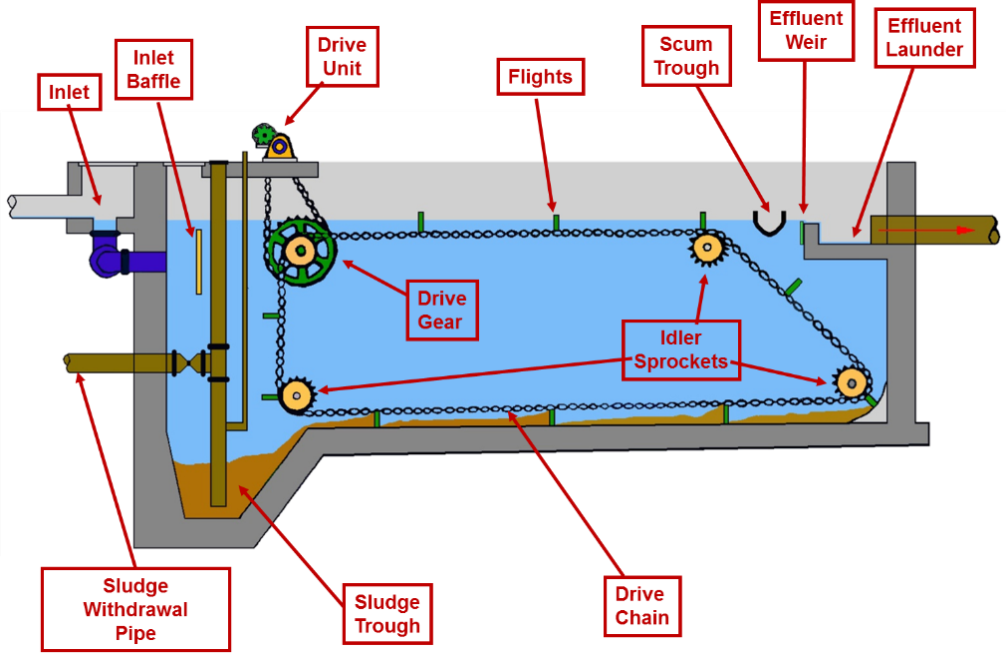
\includegraphics[scale=0.9]{RectangularClarifier}\\
				Cross section of a Rectangular Clarifier\\

				
\includegraphics[scale=0.1]{Blank}\\
				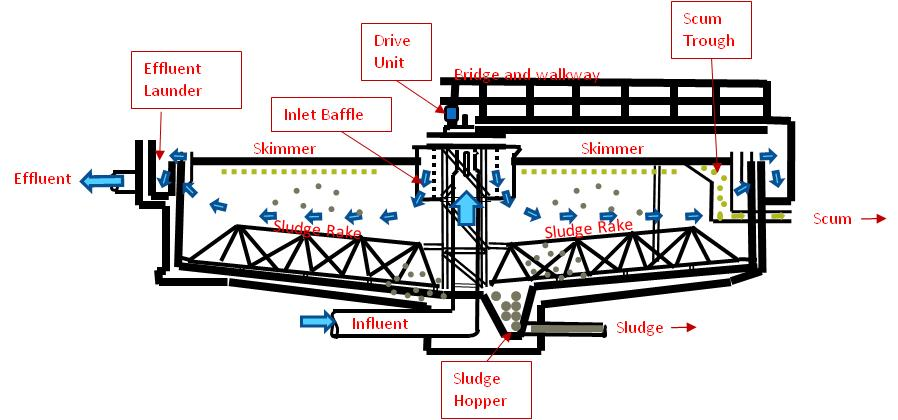
\includegraphics[scale=0.6]{CircularClarifierAI}\\
				Schematic cross section of a circular clarifier\\
				\includegraphics[scale=0.1]{Blank}\\
				\includegraphics[scale=0.5]{CircularClarifier3}\\
				Cross section of a circular clarifier\\
			\end{center}
				\includegraphics[scale=0.03]{Blank}\\
\item \textbf{Typical Removal Rates:}\\
\begin{itemize}
\item \hspace{10mm} BOD removal – 25\% to 40\% and about 60\% with CEPT
\item \hspace{10mm} Suspended solids (SS) removal – 40\% to 60\% and about 75\% with CEPT
\item \hspace{10mm} Settleable Solids removal - $>$90\%
\end{itemize}
\end{itemize}

\section{Clarifier Zones}\index{Clarifier Zones}
				
\subsection{Inlet Zone}\index{Inlet Zone}		
				\begin{itemize}
					\item Inlet Zone is where the water enters the end 					of a rectangular tank, or the center of a circular 					or square tank.
					\item The Inlet Zone is designed to accomplish two 					objectives:
						\begin{enumerate}
							\item Reduce the velocity (dissipate 									energy in the incoming water)
							\item Distribute the flow evenly
						\end{enumerate}
					\item The inlet zone is equipped with a baffle.  					Inlet baffle reduces the velocity of the 							influent flow, prevent short circuiting which 							could cause solids being carried over to secondary 					treatment.  
						\begin{itemize}
							\item Circular tanks are equipped with a 								collar-type circular baffle that directs 								the water down as it enters the center of 								the tank.
							\item Rectangular tanks will have a plate 								baffle in front of the opening for the 									wastewater flow into the clarifier and 									another baffle just upstream - a 										perforated wall or a picket fence type 									baffle that spreads the water laterally 								across the inlet end of the tank.\\


\begin{figure}[h!]
  \centering
  \begin{subfigure}[b]{0.4\linewidth}
    \includegraphics[width=0.8\linewidth]{InfluentBaffle}
    \caption{Rectangular clarifier influent baffle}
  \end{subfigure}
  \hspace{1cm}
  \begin{subfigure}[b]{0.4\linewidth}
    \includegraphics[width=\linewidth]{CircularClarifierInfluentBaffle}
    \caption{Circular clarifier influent baffle}
  \end{subfigure}
\end{figure}	
	
%							\begin{center}
%							\includegraphics[scale=0.65]												{InfluentBaffle}\\
%							Rectangular clarifier influent baffle
%							\end{center}
%							
%														\begin{center}
%							\includegraphics[scale=0.65]												{CircularClarifierInfluentBaffle}\\
%							Circular clarifier influent baffle
%							\end{center}	
						\end{itemize}
				\end{itemize}

\subsection{Settling Zone}\index{Settling Zone}
			\begin{itemize}
				\item This is the largest portion of the tank where 					solids settle.
				\item The water velocity is reduced to 0.03-0.05 fps 					and the detention time is about 1.5 to 2 hours. 
				\item A clarifier is said to be short circuiting if 					the velocity of the water is greater in some sections 					than in others. The water passing through the higher 					velocity region will have a reduced detention time and 				settleable solids will carry through with this water 					as it goes over the weir.  Short circuiting is 							prevented by appropriately designing inlet baffles and weir plates (at the Outlet Zone).
			\end{itemize}

\subsection{Sludge Zone}\index{Sludge Zone}
			\begin{itemize} 
				\item Sludge zone is the bottom of the tank where the 					settled sludge collects and compacts.
				\item Sludge blanket depth should be measured and 						sludge should be removed at least every shift. A 						desirable blanket depth is typically established and 					the sludge pumping rate and regimen is established to 					maintain that desired sludge blanket level.
				\item Sludge rakes push the sludge to one end or the 					center of the tank so that it can be pumped out. 
				\item The rake drive is usually equipped with a torque 				indicator. A shear pin in the drive shaft will break 					to prevent damage to the gearbox or drive shaft. 
				\item Failure to remove sludge often enough will 						result in the sludge becoming septic releasing gas 						bubbles which hinders the sludge settling and also 						result in causing odor problems.
				\item The sludge from the primary clarifiers needs to 					be stabilized prior to its disposal.  The sludge 						(solids) from the primary clarifiers are mixed with 					the solids from the secondary treatment process and 					stabilized typically using a sludge digestion process. 
			\end{itemize}
\subsection{Skimming Zone}\index{Skimming Zone}

			\begin{itemize}
				\item The skimming zone is at the surface of the tank 					for scum removal
				\item Lighter solids and greases float to the surface 					of the clarifier as scum
				\item In Circular Clarifiers:  Floating matter is 						skimmed by a skimmer arm that is supported by the 						sludge rake and rotates with it around the tank. The 					floating matter is pushed over the beach plate by the 					wipers attached to the skimmer arm and into a scum box 				attached to the tank wall.\\
				\item In Rectangular Clarifiers:  The flights act as 							skimmers when the chain brings them to the surface and 				pushes the scum towards the scum troughs.  The scum 					trough may be designed to rotate (tip) periodically 					for the scum to flow in from the water surface.\\
							
				\item The scum collected from the primary clarifiers is sent 				to the digester for treatment along with the sludge 					removed.\\ 

				\vspace{1cm}
									\begin{center}
					\includegraphics[scale=0.06]{RotatingScumTrough}\\
					Rectangular clarifier scum trough\\
									\includegraphics[scale=0.02]{Blank}\\
				\end{center}	

				\item The flights in the rectangular clarifier are supported 				at the top by two parallel rails running along the 						length of the clarifier.\\
				\item There are wear plates (strips) installed at the 						clarifer bottom and on top of the rails to prevent the 				flights from riding directly on those surfaces.  To 					reduce friction, the flights have a wearing shoe 						attached.  
				\item Both the wear strip and the wearing shoe 					are disposable items and are replaced at fixed 							intervals.\\			
				\begin{center}
					\includegraphics[scale=0.07]												{RectangularClarifierComponents}\\
					Rectangular clarifier flights\\
				\end{center}						  
\end{itemize}

\subsection{Outlet Zone}\index{Outlet Zone}
			\begin{itemize}
				\item  This is the part of the clarifier where the 						settled water leaves to go to the secondary treatment 					processes.
				\item A channel called the effluent launder collects 					the effluent flow and directs it to the primary 						effluent piping. 
				\item Weirs are installed along the edge of the effluent launder channel to skim the water evenly off the surface of the tank. The most common type of effluent weir is a V-notch (or saw-tooth) weir.   A V-	notch weir is a plate that has notches, about 2-3 						inches deep, cut in it every 6-8 inches. If the weir is clean and level, it will remove water evenly all 					the way around the edge of the tank. This minimizes 					the upward velocities near the effluent launder and 					improves removal efficiencies. If the weir plate is not level or part of the weir becomes clogged with 				slime or debris, short-circuiting will result because 					more water will pass over the low side or the clean notches of the weir. Short-circuiting will cause poor 					settling and uneven sludge blanket buildup.
				\item In rectangular tanks the water leaves at the end 	opposite the influent.
												  
				\item In circular  tanks the water leaves at the edge of the tank.
				\item Also, in the circular clarifiers, an effluent baffle, just upstream of the weir, 					is installed to prevent floating solids from going 						over the weir.
				\begin{center}
					\includegraphics[scale=0.04]												{CircularClarifierComponents1}\\
					Circular clarifier skimmer arm, effluent baffle and v-notch weir\\
				\end{center}
				
			\vspace{0.8cm}
					\begin{center}
					\includegraphics[scale=0.07]												{RectangularClarifierWeir}\\
					Rectangular clarifier v-notch weir and launder\\
				\end{center}			
												  
			\end{itemize}


\section{Sludge Pumping}\index{Sludge Pumping}

	\begin{itemize}
		\item The sludge pumping from the clarifier must be adequate 			to prevent sludge from going septic. Septic sludges are much 			more difficult to thicken or de-water and cause odor issues. 
		\item Primary sludge normally averages 4-6\% solids. 
		Generally positive displacement pumps are used for primary 				sludge
		\item The pumping cycles must be designed to provide the 				thickest sludge possible.
		\item Excessive pumping or pumping without building solids to 			build up leads to pumping thinner (more water) sludge.
	\end{itemize}
\section{Design Parameters}\index{Design Parameters}
	\begin{itemize}
	\setlength\itemsep{1em}
		\item \textbf{Clarifier depth} – 8 to 12 feet
		\item \textbf{Hydraulic or surface loading}
			\begin{itemize}
			\item This rate is important to ensure good settleable 					solids removal efficiency
			\item It is expressed in terms of gallons per day per 					square foot (gpd/sq ft) of tank surface area
			\item Typical surface loading rate used for the design of 				primary clarifiers range between 300 to 1,400 gpd/sq ft, 				depending on the nature of the solids and the treatment 				requirements. Lower loading rates are frequently used in 				small plants in cold climates. In warm regions, low rates 				may cause excessive detention which could lead to 						septicity.
			\end{itemize}
	\end{itemize}
\section{Math Problems}\index{Math Problems}

Types of Math Problems Related to Primary Sedimentation 

%\item Finding the clarifier hydraulic or surface loading rate
%\item Finding the clarifier detention time
%\item Finding the clarifier weir overflow rate
%\item Finding the clarifier removal efficiency
%\item Solids removal calculations
%\end{enumerate}
%\begin{enumerate}

\subsection{Hydraulic or Surface Loading Rate}\index{Hydraulic or Surface Loading Rate}

The hydraulic or surface loading rate measures how rapidly wastewater moves through the primary clarifier.  It is measured in terms of the number of gallons flowing each day through one square foot surface area of the clarifier. 
$$Clarifier \enspace hydraulic \enspace loading \enspace 	\Big(\dfrac{gpd}{ft^2}\Big) =\dfrac{Clarifier \enspace influent 	\enspace flow (gpd)}{Clarifier \enspace surface \enspace area 	(ft^2)}$$ 
		Rectangular clarifier surface area  = width * length\\
		Circular clarifier surface area  = 0.785 * Diameter$^2 $\\
\subsection{Detention Time}\index{Detention Time}

Detention time is the length of time that wastewater stays in the settling tank is called the detention time.  It is also the time it takes for a unit volume of wastewater to pass entirely through a primary clarifier\\
$$Clarifier \enspace detention \enspace time \enspace (hr) = 	\dfrac{ Clarifier \enspace volume (cu.ft \enspace or \enspace gal)}{Influent \enspace flow \enspace (cu.ft \enspace or \enspace gal)/hr)}$$
Rectangular clarifier volume = width * length * depth of water\\
Circular clarifier volume = 0.785 * Diameter$^2$ * depth of water\\
Typically volume is calculated in cu. ft and influent flow is given in gallons.  Use 7.48 gal/ft$^3$ conversion factor to convert volume in cu. ft to gallons.\\

\subsection{Weir Overflow Rate}\index{Weir Overflow Rate}
The weirs at the end of the primary clarifier allow for the even distribution of the the outlet flow across the entire length of the weir.  An adequate length of weir is needed to ensure smooth and even flow of wastewater over the weirs.  Weir overflow rate measures the number of gallons of wastewater per day flowing over one foot of weir. 

		$$Weir \enspace over \enspace flow \enspace rate \Big(\dfrac{gpd}{ft}\Big) =\Big(\dfrac{Clarifier \enspace influent \enspace  flow (gpd)}{Total \enspace effluent 					\enspace weir \enspace length \enspace (ft)}\Big)$$
		Circular clarifier weir length = 3.14 * Diameter\\

\hl{Example problem for (a), (b) and (c) above:}\\
		\vspace{0.2cm}
A circular clarifier receives a flow of 11 MGD.  If the clarifier is 90 ft. in diameter and is 12 ft. deep, what is: a) the hydraulic/surface loading rate, b) clarifier detention time in hours, and c) weir overflow rate?\\
		\vspace{0.2cm}
a) Hydraulic/surface loading rate:\\
$Clarifier \enspace hydraulic \enspace loading \enspace 	\Big(\dfrac{gpd}{ft^2}\Big) ==\dfrac{\dfrac{11\cancel{MG}}{{day}}*\dfrac{10^6gal}{\cancel{MG}}}{0.785*90^2 ft^2}=\boxed{1,730gpd/ft^2}$\\
		\vspace{0.5cm}
b) Clarifier detention time:\\
$Clarifier \enspace detention \enspace time \enspace (hr) = 	\dfrac{ Clarifier \enspace volume (cu.ft \enspace or \enspace gal)}{Influent \enspace flow \enspace (cu.ft \enspace or \enspace gal)/hr)}$\\
		\vspace{0.2cm}
$Clarifier \enspace detention \enspace time \enspace (hr) = 	\dfrac{(0.785*90^2*12)\cancel{ft^3}}{\dfrac{11\cancel{MG}}{\cancel{day}}*\dfrac{10^6\cancel{gal}}{\cancel{MG}}*\dfrac{\cancel{ft^3}}{7.48\cancel{gal}}*\dfrac{\cancel{day}}{24hrs}}=\boxed{1.2hrs}$\\
		\vspace{0.5cm}
c) Weir overflow rate:\\
		\vspace{0.2cm} 
$Weir \enspace overflow \enspace rate \Big(\dfrac{gpd}{ft}\Big) =\dfrac{\dfrac{11\cancel{MG}}{{day}}*\dfrac{10^6gal}{\cancel{MG}}}{3.14*90 ft}=\boxed{38,924gpd/ft}$\\

\subsection{Removal Efficiency}\index{Removal Efficiency}		
Primary sedimentation removes suspended wastewater solids which includes BOD.  The efficiency of the primary is established as the percentage of the amount of parameter removed.  The parameter may quantified as mass (lbs) or as concentration (mg/l).

$$Removal \enspace efficiency (\%) = \dfrac{Parameter  \enspace In - Parameter  \enspace Out}{Parameter \enspace In} * 100$$

For TSS removal:\\
$$TSS \enspace Removal \enspace efficiency (\%) = \dfrac{TSS  _{In} \enspace(mg/l)  - TSS_{Out} \enspace(mg/l)  }{TSS _{In} \enspace(mg/l)  } * 100$$

For BOD removal:\\
$$BOD \enspace Removal \enspace efficiency (\%) = \dfrac{BOD_{In} \enspace(mg/l)  - BOD_{Out} \enspace(mg/l)  }{BOD _{In} \enspace(mg/l)  } * 100$$
\subsection{Solids Removal}\index{Solids Removal}	

\hl{\textbf{Type 1 Problems:}  These involve calculating lbs of solids removed given any two of the following TSS parameters - inlet concentration, outlet concentration and removal efficiency.}\\
a. If the inlet and outlet concentrations are given, calculate the mg/l of TSS removed using: 
$$TSS_{removed} = TSS_{in}(mg/l) - TSS_{out} (mg/l) $$
Then knowing the flow, use the lbs formula to calculate the lbs solids removed.

b. If either inlet or outlet concentration is given along with the clarifier removal efficiency, using the removal efficiency calculate the unknown outlet concentration (if only the inlet is given) or the inlet concentration (if only the outlet is given)\\
i) If inlet and removal efficiency is given, calculate the outlet by subtracting the product of inlet and removal efficiency from the inlet.
$$TSS_{out}=TSS_{in} - (TSS_{in}*\%Removal)$$
Example if the removal efficiency is 60\% and the inlet concentration is 300mg/l: $$TSS_{out}=300 - 300*0.6=120mg/l$$
ii) If outlet and removal efficiency is given, calculate the inlet concentration by dividing the outlet by (1-removal efficiency).\\
$$TSS_{in}=\dfrac{TSS_{out}}{1-\%Removal}$$
Example if the removal efficiency is 60\% and the outlet concentration is 120mg/l: $$TSS_{in}=\dfrac{120}{1-0.6}=300mg/l$$ 

Note:  You may derive the above formulas by algebraically manipulating: $\%Removal=\dfrac{TSS_{in} -TSS_{out}}{TSS_{in}}$\\
\hl{Example Problem:}\\
How many lbs of solids are removed daily by a primary clarifier treating a 6 MGD flow if the average influent TSS concentration is 300 mg/l and the clarifier TSS removal efficiency is 67\%.\\
$TSS_{out}=(300mg/l - 300*0.67)=99mg/l$\\
$lbs \enspace solids \enspace  removed = (300-99)mg/l*8.34*6MGD=\boxed{10,058 \enspace lbs \enspace solids \enspace removed \enspace per \enspace day}$\\
\vspace{0.5cm}
\hl{\textbf{Type 2 Problems:}  These involve calculating the amount of sludge pumping given the solids removed.  The solids removed from the primary clarifier is sludge with a typical solids concentration of about 3\% to 5\%.}\\
Given the amount of total solids removed and given the sludge concentration, the volume of sludge pumping can be calculated as follows:  $$\dfrac{ft^3\enspace sludge\enspace pumped}{ day}= \dfrac{lbs \enspace solids \enspace (removed)}{day} * \dfrac{1 \enspace lb \enspace sludge}{(\%)\enspace lbs \enspace solids}*\dfrac{gal \enspace sludge}{8.34lb \enspace sludge}*\dfrac{ft^3 \enspace sludge}{7.48 \enspace gal} $$
So for the solids removed in the above example, if the primary sludge has 5\% solids, the required sludge pumping can be calculated as:
$$\dfrac{ft^3\enspace sludge}{day}= \dfrac{10,058 \enspace \cancel{lbs \enspace solids}}{day} * \dfrac{1 \enspace \cancel{lb \enspace sludge}}{0.05\enspace \cancel{lbs \enspace solids}}*\dfrac{\cancel{gal \enspace sludge}}{8.34\cancel{lb \enspace sludge}}*\dfrac{ft^3 \enspace sludge}{7.48 \enspace \cancel{gal}}=\boxed{3,224\dfrac{ft^3 \enspace sludge}{day}} $$

\chapterimage{QuizIcon.jpg}
\chapter{Week 3 Module Assessment Quiz}

1. An inadequate detention time in a primary clarifier would result in increased solids pumping to digesters\\

a. True \\
b. False \\

\vspace{0.3cm}
2. It is common for primary clarifiers to remove 80-85\% of the BOD and 90-95\% of the TSS.\\

a. True \\
b. False \\

\vspace{0.3cm}
3. A $\rule{1cm}{0.15mm}$ is used in the wastewater treatment plant to remove debris such as large rocks, branches, pieces of lumber, leaves, paper, tree roots etc. from the influent.\\

a. Comminutor \\
b. Bar Screen \\
c. Belt filter \\
d. Grit chamber \\

\vspace{0.3cm}
4. Grit is composed mostly of which of the following substances?\\

a. Grease \\
b. Colloidal solids \\
c. Rubber goods \\
d. Inorganics \\
e. Plastics \\

\vspace{0.3cm}
5. The following device is used to measure the flow of wastewater:

a. Comminutor \\
b. Comparator \\
c. Parshall flume \\
d. Sluice gate \\
\vspace{0.3cm}

6. If a 90 ft diameter primary clarifier operating at water depth of 20 ft is treating a 12 MGD flow, calculate the surface loading rate (gal/(day-sq.ft)\\


\vspace{0.3cm}
7. If a clarifier has a volume capacity of 0.25 MG, what is the detention time in hours if it receives a flow of 3 MGD\\


\vspace{0.3cm}
8. A grit chamber is 2 feet 4 inches wide. When wastewater is flowing 8 inches deep in this channel, the flow velocity is found to be 1.6 ft per second. Calculate flow in MGD.\\


\vspace{26cm}
\textbf{Answers:}\\
1.	b.  
\vspace{0.3cm}

2.	b.  

\vspace{0.3cm}
3.	b.  

\vspace{0.3cm}
4.	d.  

\vspace{0.3cm}
5.	c. \\ 

\vspace{0.3cm}
6.	Solution:\\
\vspace{0.3cm}
$Clarifier \enspace hydraulic \enspace loading \enspace 	\Big(\dfrac{gpd}{ft^2}\Big) =\dfrac{\dfrac{12\cancel{MG}}{{day}}*\dfrac{10^6gal}{\cancel{MG}}}{0.785*90^2 ft^2}=\boxed{1,887gpd/ft^2}$\\

\vspace{0.3cm}
7.	Solution:\\
\vspace{0.3cm}
$Clarifier \enspace detention \enspace time \enspace (hr) = 	\dfrac{ Clarifier \enspace volume (MG)}{Influent \enspace flow \enspace (MG/hr)}$\\
\vspace{0.5cm}
$Clarifier \enspace detention \enspace time \enspace (hr) = 	\dfrac{0.25\cancel{MG}}{\dfrac{3\cancel{MG}}{\cancel{day}}*\dfrac{\cancel{day}}{24hrs}}=\boxed{2hrs}$\\
\vspace{0.3cm}
8.	Solution:\\
\vspace{0.3cm}
\includegraphics[scale=0.5]{ChannelFlow3}\\
$Q=V*A$\\
$Q=1.6\dfrac{ft}{s}*\Big(\dfrac{28}{12}*\dfrac{8}{12}\Big)ft^2=2.49\dfrac{ft^3}{s}$\\
$Q=2.49\dfrac{\cancel{ft^3}}{\cancel{s}}*\dfrac{(1440*60)\cancel{s}}{day}*7.48\dfrac{\cancel{gal}}{\cancel{ft^3}}\dfrac{MG}{\cancel{gal}}=\boxed{1.61MGD}$



%\pagebreak
%\begin{center}
%|
%\vspace{10cm}
%
%BLANK PAGE
%\end{center}
%\pagebreak


%
%
\part{Week 4}
% \documentclass{article}
% %\usepackage[english]{babel}%
% \usepackage{graphicx}
% \usepackage{tabulary}
% \usepackage{tabularx}
% \usepackage[normalem]{ulem}
% \usepackage{cancel}
% \usepackage{tikz} 
% \usepackage{pdflscape}
% \usepackage{colortbl}
% \usepackage{lastpage}
% \usepackage{multirow}
% \usepackage{enumerate}
% \usepackage[shortlabels]{enumitem}
% \usepackage{color,soul}
% \usepackage{pdflscape}
% \usepackage{hyperref}
% %\usepackage[table]{xcolor}
% \usepackage{rotating}
% \usepackage{amsmath}
% \usepackage{fixltx2e}
% \usepackage{framed}
% \usepackage{mdframed}
% \usepackage[T1]{fontenc}
% \usepackage[utf8]{inputenc}
% \usepackage{textcomp}
% \usepackage{siunitx}
% \usepackage{ifthen}
% \usepackage{fancyhdr}
% \usepackage{gensymb}
% \usepackage{newunicodechar}
% \usepackage[document]{ragged2e}
% \usepackage[margin=1in,top=1.1in,headheight=57pt,headsep=0.1in]
% {geometry}
% \usepackage{ifthen}
% \usepackage{fancyhdr}
% \everymath{\displaystyle}
% \usepackage[document]{ragged2e}
% \usepackage{fancyhdr}
% \everymath{\displaystyle}
% \usepackage{empheq}

% \usepackage[most]{tcolorbox}

% \usepackage{booktabs} % Required for nicer horizontal rules in tables


% \usepackage{enumitem}

% %\usepackage[table,xcdraw]{xcolor}
% \usetikzlibrary{arrows}
% \linespread{2}%controls the spacing between lines. Bigger fractions means crowded lines%
% %\pagestyle{fancy}
% %\usepackage[margin=1 in, top=1in, includefoot]{geometry}
% %\everymath{\displaystyle}
% \linespread{1.3}%controls the spacing between lines. Bigger fractions means crowded lines%
% %\pagestyle{fancy}
% \pagestyle{fancy}
% \setlength{\headheight}{56.2pt}

% \definecolor{myblue}{rgb}{.8, .8, 1}
% \newcommand*\mybluebox[1]{%
% \colorbox{myblue}{\hspace{1em}#1\hspace{1em}}}

% \chead{\ifthenelse{\value{page}=1}{\includegraphics[scale=0.3]{SCC}\\ \textbf \textbf Wastewater Constituents Analysis \& Laboratory Methods}}
% \rhead{\ifthenelse{\value{page}=1}{}{}}
% \lhead{\ifthenelse{\value{page}=1}{}{Wastewater Constituents Analysis \& Laboratory Methods}}
% \rfoot{\ifthenelse{\value{page}=1}{Module 1: WATR 048 - Spring 2019}{Module 1: WATR 048 - Spring 2019}}

% \lfoot{Shabbir Basrai}
% \cfoot{Page \thepage\ of \pageref{LastPage}}
% \renewcommand{\headrulewidth}{2pt}
% \renewcommand{\footrulewidth}{1pt}
% \begin{document}
% %\begin{empheq}[box=\mybluebox]{align}
% %a&=b\\
% %E&=mc^2 + \int_a^a x\, dx
% %\end{empheq}

% \newlist{steps}{enumerate}{1} % Defines "Steps" for enumerate as Step 1, Step 2 etc.
% \setlist[steps, 1]{label = Step \arabic*:} % Defines "Steps" for enumerate as Step 1, Step 2 etc.

% \setlist{nolistsep} % Reduce spacing between bullet points and numbered lists


%_______________________________________________________________________________________________________________________________________%
\chapterimage{IntroductionSecondaryTreatmentImage.jpg} % Chapter heading image

\chapter{Introduction to Secondary Treatment}
\begin{itemize}
\item While preliminary and primary treatment processes are designed primarily to remove solids from wastewater, secondary treatment is for the removal of organics.
\item Secondary treatment involves:
\begin{itemize}
\item biological conversion of the dissolved and suspended organics in wastewater into biomass, and
\item physical settling (separation) process where the solids including the biomass formed during secondary treatment is separated and removed from the treated wastewater.
\end{itemize}

\item With the removal of gross solids in the preliminary treatment followed by removable of settleable solids in the primary clarifiers and the removal of dissolved and suspended organics in the secondary treatment processes, the wastewater is considered treated.
\item Secondary treated wastewater is typically disposed or treated further for reuse or disposal (depending upon the end use/application and the NPDES permit stipulations).
\item The solids (biomass) removed from the secondary treatment is typically mixed with the solids from primary treatment and stabilized using a solids treatment process like sludge digestion prior to its disposal.
\end{itemize}
\vspace{1cm}

\textbf{Secondary treatment process incorporates one of the following three approaches:}


\section{Fixed film system}\index{Fixed Film System}	

\begin{itemize}
\item Here the microorganisms responsible for the treatment, grow on substrates such
as rocks, sand or plastic.
\item When the wastewater is spread over the substrate, the microorganisms up-take the organics present in the wastewater
\item Example of this secondary treatment process include trickling filters and rotating biological contactors\\
\end{itemize}

\section{Suspended Growth System}\index{Suspended Growth System}
\begin{itemize}
\item In this type of secondary treatment, the microbes are suspended in the
wastewater flow being treated. 
\item Air or oxygen is supplied to maintain an aerobic environment and to keep the microorganisms in suspension. 
\item Example of this secondary treatment approach include the activated sludge treatment process 
\end{itemize}

\section{Pond System}\index{Pond System}
Similar to the suspended growth, stabilization ponds are large man made bodies of water which treat wastewater using mainly natural processes including sunlight, algae and microorganisms.




\chapterimage{TFChapterImage1.jpg} % Chapter heading image

\chapter{Trickling Filters}




\section{Theoretical Background}\index{Theoretical Background}
		
Trickling filter is a fixed film secondary treatment process wherein the organic content of the wastewater is removed using biological growth attached to an inert media such as lava rock or plastic\\			
\begin{itemize}
\item In a trickling filter, the wastewater is sprayed evenly on the surface of the media with a rotary type distributor with orifices
\item The wastewater percolates through the media bed, where it comes in contact with biological slime growth – zoogleal film (zooglea)
\item The aerobic biomass - bacteria, protozoa and other microoorganisms in the zooglea capture and consume the suspended and dissolved organics from the wastewater.
\item The microorganisms metabolize the organics and in the process produce more microbial mass resulting in increasing the thickness of the zoogleal layer.
\item The thickness of the zoogleal layer can only increase to a point until the wastewater flow – hydraulic load, shears the slime layer – “sloughs off” and is carried out as part of the effluent flow as sloughing.
\item The treated wastewater cascades from the bottom of the media into the underdrain system – lower portion of the TF comprised of columns which support the media base.  The underdrain has a sloping floor to direct the cascading water into a center channel .
\item The clarifier allows for the separation (settling) of the  of the solids (sloughed off material).  The settled solids is removed - typically pumped to a digester and the clarified effluent flows out of the clarifier.
\item The source of oxygen to support the aerobic growth is from the oxygen dissolved in the wastewater as it is sprayed over the media and from the air currents due to the downward flow of the wastewater and the temperature difference between ambient and the interior of the trickling filter.  Forced ventilation system may be designed as part of the trickling filter

\item Word trickling “filter” is a misnomer - no filtration is involved
\item Advantage includes process simplicity and lower costs
\item Disadvantage include BOD removal efficiency of only about 80-85%
\item The media may be rock, slag, coal, bricks, redwood blocks, molded plastic, or any other sound durable material.
\item The media depth ranges from about three to eight feet for rock media trickling filters and 15 to 30 feet for synthetic media.
\item The media needs to be uniformly sized and have adequate empty spaces (voids) to ensure maintaining aerobic condition necessary for the survival of biomass.  

\item Pre-fabricated (synthetic) media - similar to the one shown below, has an advantage over the "dumped" type media such as lava rock of providing a greater surface area per volume upon which the zoologeal film may grow while providing ample void space for the free circulation of air.

\item Sometimes, due to inadequate hydraulic loading, portions of the zoogleal layer may become too thick and oxygen cannot penetrate its full depth, causing odor issues.

\end{itemize}


\section{Trickling Filter Recirculation}\index{Trickling Filter Recirculation}

Recirculation - where a portion of the treated wastewater is returned back as the feed to the TF.  The parameter recirculation ratio is calculated to quantify the recirculation flow.  Recirculation ratio is a ratio of the recirculated flow - Q$_R$ to the influent flow Q$_I$. Recirculation ratios typically vary from 0.5 to 4.
\begin{center}
\includegraphics[scale=0.5]{TFrecirculation}
\end{center}
Recirculation is beneficial for the following reasons:
\begin{itemize}
\item It improves the removal efficiency by increasing the contact time of the zoogleal layer with the wastewater
\item During low flows it prevents the trickling filter from drying out
\item It dilutes any toxic loadings
\item It promotes oxygen transfer and reduces ponding
\item The increased hydraulic loading promotes uniform sloughing, prevents ponding, improves ventilation through the filter and reduces potential for snail and filter fly breeding
\end{itemize}
\section{Operation of Multiple Trickling Filters}\index{Operation of Multiple Trickling Filters}

Multiple trickling filters can be operated in series or in parallel:\\
\begin{itemize}
\item Series operation in which the flow from one flows into the next.
\begin{center}
\includegraphics[scale=0.5]{TFSeries1}
\end{center}  
\begin{itemize}
\item For high strength loading and for nitrification
\end{itemize}
\item Parallel operation in which the trickling filters that are operated side by side.
\begin{center}
\includegraphics[scale=0.6]{TFParallel1}
\end{center}
\begin{itemize}
\item For winter operation - prevents freezing in the TF
\end{itemize}
\end{itemize}

\section{Parameters for monitoring and operating trickling filters}\index{Parameters for monitoring and operating trickling filters}



\begin{enumerate}
\item Hydraulic loading is expressed as gpd/$ft^2$
\item BOD Removal (\%)
\item Organic loading lbs BOD/day/ 1000 cu ft
\item Recirculation ratio
\end{enumerate}


\section{Classifying Trickling Filters}\index{Classifying Trickling Filters}			
Trickling filters are classified according to the hydraulic and organic loading applied to the  filter\\

\subsection{Low-rate filter}\index{Low-rate filter}

\begin{itemize}
\item The standard rate or low rate trickling filters (LRTF) are relatively simple treatment units that normally produce a consistent effluent quality even with varying influent strength
\item They are generally not provided with recirculation of effluent
\item Depending upon the dosing system, wastewater is applied intermittently with rest periods which generally do not exceed five minutes at the designed rate of waste flow. 
\item While there is some unloading or sloughing of solids at all times, the major unloadings usually occur several times a year for comparatively short Periods of time.
\end{itemize}

     Hydraulic loading is 25 - 100 gal/day/sq. ft\\
     BOD Removal (\%) 	50 – 80\%\\
     Organic loading is 5 - 25 lbs BOD/day/1000 cu ft\\

\subsection{High-rate filter}\index{High-rate filter}

\begin{itemize}
\item The most important element of a high-rate trickling filter is the provision where a part of the settled treated effluent is pumped to the PST or to the filter.  This is termed as \textbf{Recirculation}
\item High-rate filters are usually characterized by higher hydraulic and organic loadings than low-rate filters
\item The higher BOD loading is accomplished by applying a larger volume of waste per unit surface area of the filter.  \item As a result of the higher flow velocities a more continuous and uniform sloughing of excess zoogleal growth occurs
\end{itemize}

     Hydraulic loading is 100 - 1000 gal/day/sq. ft\\
     BOD Removal (\%) 	65 - 85\%\\
     Organic loading is 25 - 100 lbs BOD/day/ 1000 cu ft\\
			
\subsection{Roughing filter}\index{Roughing filter}

\begin{itemize}
\item Roughing filters are high rate type filters designed with plastic packing
\item In most cases roughing filters are used to treat wastewater prior to secondary treatment
\item One of the advantages of roughing filter is low energy requirement for BOD removal of high strength wastewaters as compared to activated sludge process because the energy required is only for pumping the influent wastewater and recirculation flows
\end{itemize}



\section{Trickling Filter Operational Issues}\index{Trickling Filter Operational Issues}

\subsection{Ponding}\index{Ponding}


If the voids in the media get plugged, flow can collect on the surface in ponds.
Correction:
spraying the surface with high pressure water stream
stopping a rotary distributor over the ponded area
hand-stir the media or open the voids
dose the filter with chlorine for several hours

\subsection{Odors}\index{Odors}


\begin{itemize}
\item Corrective measures should be taken immediately if foul odors develop
\item presence of foul odors indicates anaerobic conditions are predominant
\item Check the under drain system for obstructions or heavy biological growths
\item increase the recirculation rate to provide more oxygen to the filter bed and increase sloughing 
\item keep slime growths off of sidewalks and inside walls of the filter to reduce the odor
\end{itemize}

\subsection{Trickling Filter Flies - Psychoda}\index{Trickling Filter Flies - Psychoda}

\begin{itemize}
\item tiny, gnat-size filter fly, or Psychoda - primary nuisance insect
\item Correction methods include
\begin{itemize}
\item Increase recirculation rate
\item keep orifice openings clear
\item apply insecticides to filter walls
\item dose filter with chlorine
\item keep weeds and tall grass cut around filter
\end{itemize}
\end{itemize}


\subsection{Cold weather problems}\index{Cold weather problems}

\begin{itemize}
\item ice can form on the media of the filter
\item Correction methods include:
\begin{itemize}
\item decrease recirculation to the filter (influent is usually warmer than recycled flows)
\item construct wind screens
\item operate two-stage filters in parallel rather than in series
\end{itemize}
\end{itemize}


\section{Math Problems}\index{Math Problems}

Trickling filter problems involve calculation of the following:

\subsection{Hydraulic or surface loading}\index{Hydraulic or surface loading}

\begin{itemize}
\item Hydraulic or surface loading is expressed as gpd/$ft^2$
\item \hl{The gpd is the total flow (Q$_T$)to the filter - primary influent flow + recirculated flow(Q$_T$= Q$_I$ + Q$_R$)}\\
\end{itemize}
			\hl{Example Problem:}\\
The total influent flow (including recirculation) to a trickling filter is 1.89 MGD. If the trickling filter is 80 ft in diameter, what is the hydraulic loading in gpd/sq ft on the trickling filter?\\
\vspace{0.2cm}
Solution:\\
\vspace{0.2cm}
$Hydraulic \enspace loading \enspace \dfrac{gpd}{ft^2}=\dfrac{(1.89*10^6)gpd}{(0.785*80^2)ft^2} =\boxed{376\dfrac{gpd}{ft^2}}$
			
			
\subsection{BOD and TSS Removal}\index{BOD and TSS Removal}
BOD and  removal is based upon the TF influent and effluent concentrations.\\
\vspace{0.2cm}
$\% Removal=\dfrac{In_{conc}-Out_{conc}}{In_{conc}}*100$\\
			\hl{Example Problem:}\\
The suspended solids concentration entering a trickling filter is 236 mg/l. If the suspended solids concentration of the trickling filter effluent is 33 mg/l, what is the suspended solids removal efficiency of the trickling filter?\\
\vspace{0.2cm}
Solution:\\
\vspace{0.2cm}
$\% Removal=\dfrac{236 mg/l-33 mg/l}{236 mg/l}*100=\boxed{86\%}$

\subsection{Organic Loading}\index{Organic Loading}

			\begin{itemize}
\item Organic loading to a trickling filter is typically expressed as lbs BOD/(day-1000 cu ft).  \item The lbs/day BOD value is the BOD loading from the primary effluent.
\item The 1000 ct. ft is the volume of the media.  
\item The media volume is calculated by multiplying the TF surface area by the media height.  
\item As the dimensions are typically given in ft., calculate the volume in $ft^3$ and then divide the calculated volume by 1000 to give the volume in units of 1000$ft^3$\\
\end{itemize}
\hl{Example Problem:}\\
A trickling filter, 70 ft in diameter with a media depth of 6 ft, receives a flow of 0.78 MGD. If the BOD concentration of the primary effluent is 167 mg/L, what is the organic loading on the trickling filter in lbs BOD/day/1000 cu ft?\\
Solution:  $Organic \enspace loading:\dfrac{lbs \enspace BOD}{day-1000ft^3}=\dfrac{lbs \enspace BOD \enspace feed \enspace to \enspace TF \enspace per \enspace day}{volume \enspace in \enspace 1000ft^3}$\\
$=\dfrac{\dfrac{(0.78*167*8.34)lbs \enspace BOD}{day}}{(0.785*70^2*6)ft^3*\dfrac{1000ft^3}{1000ft^3}}=\boxed{\dfrac{47 lbs \enspace BOD}{day-1000 ft^3}}$

\subsection{Recirculation Ratio}\index{Recirculation Ratio}


$Recirculation \enspace Ratio (R_R)=\dfrac{Recirculated \enspace Flow (Q_R)}{Influent  \enspace  Flow (Q_I)}$\\
\vspace{0.5cm}
$Recirculation \enspace Ratio (R_R)=\dfrac{Total \enspace Flow (Q_T) - Influent \enspace Flow (Q_I)}{Influent  \enspace  Flow (Q_I)}$\\
\vspace{0.5cm}
$Total \enspace Flow (Q_T) = Influent \enspace Flow (Q_I)*(Recirculation \enspace Ratio(R_R) +1)$
Make sure $Q_R$, $Q_T$ and $Q_I$ units are the same in a given problem

\hl{Example Problems:}\\
\begin{enumerate}
\item The influent to the trickling filter is 1.61 MGD. If the recirculated flow is 2.27 MGD, what is the recirculation ratio?\\
\vspace{0.2cm}
Solution:  $R_R=\dfrac{Q_R}{Q_I}=\dfrac{2.27}{1.61}=\boxed{1.4}$\\
\vspace{0.2cm}
\item A trickling filter has a total flow of 32 MGD.  If the recirculation ratio is 0.8, what is the primary effluent flow to the TF?\\
\vspace{0.2cm}
Solution:\\
\vspace{0.2cm}
$Total \enspace Flow (Q_T) = Influent \enspace Flow (Q_I)*(Recirculation \enspace Ratio(R_R) +1)$\\
$\implies 32 MGD=Q_I*(0.8+1)\implies Q_I=\dfrac{32}{1.8}=\boxed{17.8 MGD}$
\end{enumerate}
\newpage
\chapterimage{QuizIcon.jpg}
\chapter{Week 4 Module Assessment Quiz}

1. The main purpose of the trickling filter media is to provide nutrients to the zoogleal mass growing on it\\

a. True \\
b. False \\
\vspace{0.3cm}

2. The advantage of trickling filter over the activated sludge lies in its BOD removal efficiency 

a. T\\

b. F\\

\vspace{0.3cm}

3. A good reason to run a trickling filter in the series mode of operation is:\\

a. During cold weather to prevent ice formation \\
b. When the influent BOD loading is low \\
c. When the influent BOD loading is high \\
d. When the weather is warm \\

\vspace{0.3cm}
4. If a trickling filter has been operating with a hydraulic loading (including some recirculation) of 10 to 12 MGD and organic loading of about 80 pounds of BOD per 1,000 cu. ft./day the treatment efficiency will usually increase if the recirculation is increased. This might be attributed to:

a. The increased recirculation wears down the soluble BOD to finer particles \\
b. The increased flow more completely wets and contacts all of the slime surfaces in the filter so the food to effective microorganism ration is less as in an activated sludge process \\
c. The grazing population of warm and other organisms in the filter is flushed out before they consume the slime bacteria \\
d. The increased flow more completely fills the under drains so cold updrafts are eliminated\\ 
e. The statement is just poppycock put out by power companies to get us to use more electricity to run pumps \\
\vspace{0.3cm}

5. The primary organisms responsible for treating wastewater in the trickling filter process are:\\

a. Anaerobic bacteria \\
b. Anoxic bacteria \\
c. Facultative bacteria \\
d. Aerobic bacteria \\
\vspace{0.3cm}

6. Sloughing from a trickling filter refers to\\

a. A process whereby wastewater is recirculated over the filter. \\
b. Bypassing of the filter. \\
c. The breaking of the filter stone as a result of weathering and the sluicing of small stone particles to the final settling tank. \\
d. The discharge of slime growth with the filter effluent. \\

\vspace{0.3cm}
7. Which of the following is not a benefit of recirculation in the trickling filter process?\\

a. Dilutes high strength or toxic wastes. \\
b. Helps prevent septic conditions in trickling filter \\
c. Helps prevent excessive sloughing \\
d. Helps control odors, ponding and filter flies \\

\vspace{0.3cm}
8. Calculate the organic load in lbs of BOD/day/1000 cu. ft. for a trickling filter 50 ft in diameter and eight (8) ft deep. Given a flow of 250,000 gpd, and a 150 mg/l BOD concentration of the primary effluent feed to the trickling filter.\\

a. 2 lbs/day/1000 cu. ft. \\
b. 5 lbs/day/1000 cu. ft. \\
c. 20 lbs/day/1000 cu. ft. \\
d. 50 Ibs/day/1000 cu. ft. \\
\vspace{0.3cm}

9. A trickling filter plant operating at a recirculation ratio of 1 receives a raw wastewater flow of 2 MGD. This means that the flow being applied to the filter would be:

a. 4mgd. \\
b. 1mgd \\
c. 3mgd \\
d. 2mgd \\
e. 6mgd \\


\vspace{1cm}
\textbf{Answers:}\\
1.	b.  

\vspace{0.3cm}
2.	b.  

\vspace{0.3cm}
3.	c.  
\vspace{0.3cm}

4.	b.  

\vspace{0.3cm}
5.	d.  

\vspace{0.3cm}
6.	d.  
\vspace{0.3cm}

7.	c.  
\vspace{0.3cm}
\newpage
8.	c.  

\vspace{0.3cm}

Solution:\\
\vspace{0.5cm}
$Organic \enspace loading:\dfrac{lbs \enspace BOD}{day-1000ft^3}=\dfrac{lbs \enspace BOD \enspace feed \enspace to \enspace TF \enspace per \enspace day}{volume \enspace in \enspace 1000ft^3}$\\
\vspace{0.5cm}
$=\dfrac{\dfrac{(0.25*150*8.34)lbs \enspace BOD}{day}}{(0.785*50^2*8)ft^3*\dfrac{1000ft^3}{1000ft^3}}=\boxed{\dfrac{20 lbs \enspace BOD}{day-1000 ft^3}}$
\vspace{0.3cm}
9.	c.  

\vspace{0.3cm}

Solution:\\
\vspace{0.5cm}
$Recirculation \enspace Ratio (R_R)=\dfrac{Recirculated \enspace Flow (Q_R)}{Influent  \enspace  Flow (Q_I)}$\\
\vspace{0.5cm}
$ \implies 1=\dfrac{Recirculated \enspace Flow (Q_R)}{2MGD} \implies Recirculated \enspace Flow (Q_R)=2MGD$\\
$\implies Flow \enspace to \enspace TF= Recirculated \enspace Flow (Q_R)+Influent  \enspace  Flow (Q_I)=2+2=\boxed{4MGD}$

\part{Week 5}
% \documentclass{article}
% %\usepackage[english]{babel}%
% \usepackage{graphicx}
% \usepackage{tabulary}
% \usepackage{tabularx}
% \usepackage[normalem]{ulem}
% \usepackage{cancel}
% \usepackage{tikz} 
% \usepackage{pdflscape}
% \usepackage{colortbl}
% \usepackage{lastpage}
% \usepackage{multirow}
% \usepackage{enumerate}
% \usepackage[shortlabels]{enumitem}
% \usepackage{color,soul}
% \usepackage{pdflscape}
% \usepackage{hyperref}
% %\usepackage[table]{xcolor}
% \usepackage{rotating}
% \usepackage{amsmath}
% \usepackage{fixltx2e}
% \usepackage{framed}
% \usepackage{mdframed}
% \usepackage[T1]{fontenc}
% \usepackage[utf8]{inputenc}
% \usepackage{textcomp}
% \usepackage{siunitx}
% \usepackage{ifthen}
% \usepackage{fancyhdr}
% \usepackage{gensymb}
% \usepackage{newunicodechar}
% \usepackage[document]{ragged2e}
% \usepackage[margin=1in,top=1.1in,headheight=57pt,headsep=0.1in]
% {geometry}
% \usepackage{ifthen}
% \usepackage{fancyhdr}
% \everymath{\displaystyle}
% \usepackage[document]{ragged2e}
% \usepackage{fancyhdr}
% \everymath{\displaystyle}
% \usepackage{empheq}

% \usepackage[most]{tcolorbox}

% \usepackage{booktabs} % Required for nicer horizontal rules in tables


% \usepackage{enumitem}

% %\usepackage[table,xcdraw]{xcolor}
% \usetikzlibrary{arrows}
% \linespread{2}%controls the spacing between lines. Bigger fractions means crowded lines%
% %\pagestyle{fancy}
% %\usepackage[margin=1 in, top=1in, includefoot]{geometry}
% %\everymath{\displaystyle}
% \linespread{1.3}%controls the spacing between lines. Bigger fractions means crowded lines%
% %\pagestyle{fancy}
% \pagestyle{fancy}
% \setlength{\headheight}{56.2pt}

% \definecolor{myblue}{rgb}{.8, .8, 1}
% \newcommand*\mybluebox[1]{%
% \colorbox{myblue}{\hspace{1em}#1\hspace{1em}}}

% \chead{\ifthenelse{\value{page}=1}{\includegraphics[scale=0.3]{SCC}\\ \textbf \textbf Wastewater Constituents Analysis \& Laboratory Methods}}
% \rhead{\ifthenelse{\value{page}=1}{}{}}
% \lhead{\ifthenelse{\value{page}=1}{}{Wastewater Constituents Analysis \& Laboratory Methods}}
% \rfoot{\ifthenelse{\value{page}=1}{Module 1: WATR 048 - Spring 2019}{Module 1: WATR 048 - Spring 2019}}

% \lfoot{Shabbir Basrai}
% \cfoot{Page \thepage\ of \pageref{LastPage}}
% \renewcommand{\headrulewidth}{2pt}
% \renewcommand{\footrulewidth}{1pt}
% \begin{document}
% %\begin{empheq}[box=\mybluebox]{align}
% %a&=b\\
% %E&=mc^2 + \int_a^a x\, dx
% %\end{empheq}

% \newlist{steps}{enumerate}{1} % Defines "Steps" for enumerate as Step 1, Step 2 etc.
% \setlist[steps, 1]{label = Step \arabic*:} % Defines "Steps" for enumerate as Step 1, Step 2 etc.

% \setlist{nolistsep} % Reduce spacing between bullet points and numbered lists


%_______________________________________________________________________________________________________________________________________%
\chapterimage{Week5Ponds.jpg} % Chapter heading image

\chapter{Stabilzation Ponds}
% Chapter heading image

\begin{itemize}
\item Stabilization ponds and lagoons are bodies of water which treat wastewater using mainly natural processes including sunlight, algae and microorganisms for treating wastewater\\
\item While ponds are shallow and man-made, lagoons are bodies of water confined within natural boundaries.\\
\end{itemize}


\section{Advantages of ponds}\index{Advantages of ponds}	

\begin{itemize}	
\item Cheap to build and operate
\item Low maintenance and electrical costs
\item Do not require highly trained operational personnel
\item Provide treatment that can be equal to some secondary treatment processes and have fewer sludge handling issues.\\
\end{itemize}


\section{Disadvantages of ponds}\index{Disadvantages of ponds}	
\begin{itemize}	
\item Land intensive
\item Effluent quality varies with seasonal temperature changes
\item Suspended solids levels that can create regulatory problems.
\item System upsets almost always result in odor problems and recovery times may be weeks or months.
\item Not appropriate for colder climates
\end{itemize} 

\section{Types of Ponds}\index{Types of Ponds}	

\subsection{Anaerobic Ponds}\index{Anaerobic Ponds}	

\begin{itemize}	
\item Typically for treating raw sewage
\item Designed for BOD removal
\item 10-14 feet deep. 
\item High strength wastewater may be treated
\item Utilize anaerobic bacteria to break down the organic waste. 
\item Septic conditions in the lagoon and odors associated with septic sewer gases particularly hydrogen sulfide and its rotten egg odor. 
\item Most of the decomposition is accomplished by acid forming bacteria. 
\item The pH in these lagoons is usually below 6.5. 
\item They are total retention and do not have an effluent discharge. 
\item The anaerobic pond must be de-sludged approximately once every 2 to 5 years
\item Organic loading of 200-1000 lbs. $BOD_5$ per acre per day
\end{itemize}

\subsection{Facultative Ponds}\index{Facultative Ponds}	

\begin{itemize}
\item Typically for secondary treatment - BOD removal
\item Are about 4-7 feet deep
\item 15-50 lbs $BOD_5$ per acre per day.
\item Facultative bacteria are responsible for most of the treatment that occurs in these ponds (facultative bacteria can live under both aerobic and anaerobic conditions)
\item Most common design for lagoon systems that are used to treat raw wastewater. 
\item Designed for a BOD loading rate of 20-35 pounds per acre per day – about 1 surface acre for about 300 – 400 people
\item Suspended solids settle to the bottom of the pond where there is less dissolved oxygen.  
\item The facultative bacteria will become anaerobic to digest these solids. Circulation in the pond will eventually bring these bacteria to the surface where high levels of dissolved oxygen exist. When this occurs, the bacteria will become aerobic to stabilize the dissolved organics that are present.
\item The algae that grow in the lagoon are critical to the successful stabilization of the organic load. 
\item The algae will take in carbon dioxide ($CO_2$) and, through photosynthesis, use it to create sugars and release dissolved oxygen ($O_2$) that is used by the aerobic bacteria. Facultative lagoon levels should always maintain at least 4 feet of water in the pond.
\item Unused CO$_2$ will react with water to form carbonic acid - which would reduce the pH unless consumed
\item When the sun goes down, photosynthesis stops. Since there is no uptake of carbon dioxide at night, the pH of the lagoon will slowly drop back to 6.8-7.0.
\item During the day the pH will gradually rise to about 7.2 – 7.6 as the $CO_2$ is consumed
\item \hl{The lowest pH will be just before dawn} 
\item An indication of an overloaded pond is its low pH as the $CO_2$ produced by the bacteria is not consumed by the algae quickly enough
\item Detention times range from 30-60 days. Raising or lowering the operating level can change detention times
\item Sludge removal need is rare.  Sludge can be removed by using a raft-mounted sludge pump or by draining and dewatering the pond and removing the sludge with a front-end loader.
\end{itemize} 

				\begin{sidewaysfigure}
\begin{center}
\includegraphics[scale=0.8]{StabilizationPond}\\
Facultative pond schematic
\end{center}
				\end{sidewaysfigure}
				
\subsection{Aerobic Stabilization Ponds}\index{Aerobic Stabilization Ponds}
	
Aerobic stabilization ponds are also known as: \hl{maturation}, \hl{polishing} or \hl{finishing} Pond
\begin{itemize}
\item Typically for tertiary treatment
\item Designed for pathogen removal
\item Shallow - only about 3 feet deep. 
\item They are most often the final cells in a multi-staged pond system
\item They are also used as polishing ponds for tertiary treatment of trickling filter plant effluent.
\item Usually the effluent is directed into a second pond where the sludge can settle 
\item Their shallow depth allows sunlight to penetrate to the bottom of the pond to encourage algae growth and aerobic conditions throughout the pond 
\item The low solids loading found in these tertiary treatment applications means that these ponds normally have no sludge zone
\item These ponds may be mechanically aerated 
\item Aerobic polishing ponds are designed for 15-20 pounds BOD/acre/day
\item Aerobic ponds are typically designed for pathogen removal
\item Aerobic lagoon levels should always maintain at least 18 inches of water in the pond
\end{itemize}



\section{Ponds Operations and Maintenance}\index{Ponds Operations and Maintenance}

\begin{itemize}
\item Ponds and lagoons are designed as continuous discharge, controlled discharge, or no discharge.
\begin{itemize}
\item In controlled discharge ponds the wastewater is held for long periods of time before discharging. 

\item No-discharge ponds the inflow rate needs to be equal or exceed the rates of evaporation and/or percolation. 
\end{itemize}
\item Short-circuiting in a pond may be caused by poor design of inlet and outlet piping arrangements or by uncontrolled growth of water weeds.
\item Stagnant water will breed mosquitoes and can result in anaerobic conditions developing that can cause odor issues 
\item Dikes need to be maintained
\item Aquatic plants and weeds must be removed from the water. 
\item Reeds will create stagnant areas along the edge of the pond and need to be removed
\item To start a new pond, two feet of water is typically added prior to fresh starting wastewater feed. 
\item Sodium nitrate can be used to help recover from an odor-causing upset. The nitrates ($NO_3$) will provide a source of chemically bound oxygen for the bacteria to use instead of dissolved oxygen.
\item Scum control may be required
\end{itemize}

\section{Math Problems}\index{Math Problems}

\subsection{Pond Area}\index{Pond Area}

Formula: \hl{$Pond \enspace Area=Width * Length$}\\
\vspace{0.2cm}
also,     \hl{$Pond \enspace Area=\dfrac{Pond \enspace Volume}{Pond \enspace Depth}$}\\
\vspace{0.2cm}
\hl{Example Problem:}\\
A pond is 260 ft. long and 80 ft. wide. What is the area of this pond in acres?\\ 
\vspace{0.2cm}
Solution:\\
\vspace{0.2cm}
$(260*80)ft^2*\dfrac{acre}{43,560ft^2}=\boxed{0.48acre}$

\subsection{Solids Loading Rate}\index{Solids Loading Rate}


Formula: \hl{$Pond \enspace TSS \enspace loading \enspace rate =  \dfrac{lbs \enspace TSS}{day}$}  \\
\vspace{0.3cm}
\hl{Example Problem:}\\
\vspace{0.3cm}

The influent flow to a pond is 10,000 gallons/hour with a suspended solids concentration of 142mg/L in the raw wastewater.  How many lbs of suspended solids are sent to the pond daily?
\\
Solution:\\
\vspace{0.3cm}
$\dfrac{lbs \enspace TSS}{day}=10,000\dfrac{gal}{hr}*\dfrac{24hrs}{day}*\dfrac{MG}{1,000,000gal}*142\dfrac{mg}{l}*8.34=\boxed{284\dfrac{lbs \enspace TSS}{day}}$

\vspace{0.3cm}

\subsection{Organic Loading Rate}\index{Organic Loading Rate}

\vspace{0.3cm}
Formula: \hl{$Pond \enspace organic \enspace loading \enspace rate =  \dfrac{lbs \enspace BOD/day}{Area (acre)}$}  \\
\vspace{0.3cm}
\hl{Example Problem:}\\
\vspace{0.3cm}
The flow to a pond is 7.2MGD. If the pond diameter is 350 ft and the BOD in the pond influent is 170mg/L, what is the organic loading to this pond in lbs BOD/day/acre?
\\
Solution:\\
\vspace{0.3cm}
$Organic \enspace loading=\dfrac{lbs \enspace BOD \enspace per \enspace day}{area \enspace (acres)}=\dfrac{(7.2MGD \enspace * \enspace 170mg/l \enspace * \enspace 8.34)}{0.785*350^2ft^2}*\dfrac{43,560ft^2}{acre}=\boxed{\dfrac{4,624lbs \enspace BOD}{day-acre}}$

\vspace{0.3cm}

\subsection{Detention time}\index{Detention time}
\vspace{0.3cm}
Formula: \hl{$Pond \enspace detention \enspace time=\dfrac{Volume}{Flow}$}\\ 
\vspace{0.3cm}
\hl{Example Problem:}\\
A 40 acre wastewater treatment pond receives a flow of 0.6 MGD. If the pond is operated at a depth of 4ft. What is the detention time of this pond?\\
Solution:\\
$Pond \enspace detention \enspace time=\dfrac{Volume}{Flow}=\dfrac{(40*4)acre-ft}{0.6*10^6\dfrac{gal}{day}*\dfrac{ft^3}{7.48gal}*\dfrac{acre-ft}{43,560ft^3}}=\boxed{87 \enspace days}$\\
\vspace{0.3cm}


\subsection{Hydraulic Loading Rate}\index{Hydraulic Loading Rate}
Formula:\hl{$Pond \enspace hydraulic \enspace loading \enspace rate \enspace \Bigg[\dfrac{in}{day}\Bigg]=\dfrac{Flow}{Area}$}\\
also, \hl{$Pond \enspace hydraulic \enspace loading \enspace rate \Bigg[\dfrac{in}{day}\Bigg]=\dfrac{Pond \enspace depth \enspace (in)}{Pond \enspace detention  \enspace time \enspace \dfrac{Volume}{Flow}}$ }\\
The second formula above is because:\\
\vspace{0.3cm}
$Hydraulic \enspace Loading \enspace (HL)=\dfrac{Flow}{Area}$\\
\vspace{0.3cm}
$Detention \enspace time \enspace (DT)=\dfrac{Vol}{Flow} \implies Flow=\dfrac{Vol}{DT} $\\
\vspace{0.3cm}
Substituting for flow in  the HL formula above:\\
\vspace{0.3cm}
$HL=\dfrac{\dfrac{Vol}{DT}}{Area}\enspace or \enspace \dfrac{Vol}{Area*DT} \enspace \implies \boxed{HL=\dfrac{Pond \enspace Depth}{DT}} \enspace as \enspace \dfrac{Vol}{Area}=Pond \enspace Depth$\\
\vspace{0.3cm}
\textbf{Example Problems:}\\
\begin{enumerate}

\item Find hydraulic loading in inches/day for a pond given the following:
\begin{itemize}
\item Pond depth = 12ft.
\item Pond volume = 1,400,000ft3
\item Pond flow = 1,000,000gal/day
\end{itemize}
Solution:\\
$Pond \enspace hydraulic \enspace loading \enspace rate \enspace \Bigg[\dfrac{in}{day}\Bigg]=\dfrac{Flow}{Area}$\\
$ \implies\dfrac{1,000,000\dfrac{gal}{day}*\dfrac{ft^3 }{7.48gal}}{\dfrac{1,400,000ft^3}{12ft}}*12\dfrac{in}{ft}=\boxed{13.8\dfrac{in}{day}}$\\
\vspace{0.3cm}
\hl{Note:  The area of the pond was found by dividing the volume (1,000,000$ft^3$) by the pond depth (12ft)}
\vspace{0.3cm}

\item Find pond hydraulic loading in inches/day when the depth of the pond is 6 ft. and the detention time is 30 days.\\
Solution:\\



$Pond \enspace hydraulic \enspace loading \enspace rate=\dfrac{Pond \enspace depth \enspace (in)}{Pond \enspace detention  \enspace time \enspace \dfrac{Volume}{Flow}}$\\
$\implies \dfrac{6*12 \enspace inches}{30 \enspace days}=\boxed{\dfrac{2.4in}{day}}$
\end{enumerate}




\chapterimage{Week5AS.jpg} % Chapter heading image

\chapter{Activated Sludge}


\section{Activated Sludge Basics}\index{Activated Sludge Basics}

Activated sludge is a secondary, biological treatment process used for the removal of suspended and dissolved organic matter from the primary treated wastewater.
\begin{itemize}
\item Utilizes an aeration basin/reactor and a secondary clarifier

\item In the presence of oxygen, aerobic bacteria in the aeration basin consume the organic matter (BOD) in wastewater for their growth and reproduction, converting BOD into bacterial cell mass along with metabolic byproducts including carbon dioxide and water

\item The aerobic bacteria is the predominant microbial life form in the aeration basin.  Other higher microbial life forms — mainly protozoa, are present along with some metazoans.

\item The microorganisms along with their metabolic byproducts and residual dead cell mass form a cluster called floc.

\item The wastewater exiting the aeration basin enters a clarifier where the floc settles.  The clear, treated secondary effluent flows out.

\item A portion of the settled activated sludge floc, is returned from the clarifier to the front of the aeration basin to seed the activated sludge treatment of the incoming primary effluent. The recycled floc is called \textbf{Return Activated Sludge (RAS)}.

\item The remaining settled floc from the clarifier is ”wasted” \textemdash transferred for solids treatment (typically using digestion) prior to its ultimate disposal. The wasted floc is called \textbf{Waste Activated Sludge (WAS)}.

\item The color of healthy activated sludge is tan to brown with an earthy/musty odor.

\begin{center}
\includegraphics[scale=0.48]{ASProcess}
\end{center}

\item For activated sludge treatment to be effective, it is critical to establish a healthy microbial population which \hl{converts the BOD} into \hl{easily separable biomass.}
\item If the biomass does not settle well in the clarifier, it will be carried out in the treated secondary effluent producing a poor quality effluent with higher solids and organic content.  \\
\end{itemize}

    \begin{mdframed}[backgroundcolor=blue!20] 
\textbf{Mixed liquor}:
\begin{itemize}
\item Mixed liquor is the mixture of raw and/or treated wastewater with the biomass.
\item Mixed liquor sample is typically taken at the end of the aeration reactor.
\item In the mixed liquor, the suspended solids comprised mostly of biomass with some undegraded and non-degradable material is called \textbf{Mixed liquor suspended solids (MLSS)}.  
\item The volatile fraction of the MLSS is termed \textbf{Mixed Liquor Volatile Solids (MLVSS)}.  \item The MLVSS is the amount of biomass as a percentage of the MLSS.  Typically, MLVSS is 70 - 80\%, implying that 70-80\% of the MLSS is volatile (organic) solids.
\end{itemize}
    \end{mdframed}

\section{Activated Sludge Process Control Parameters}\index{Activated Sludge Process Control Parameters}

\subsection{Dissolved Oxygen}\index{Dissolved Oxygen}

Maintaining adequate \textbf{Dissolved oxygen (DO)} is key to the activated sludge process.  DO is typically maintained between 0.5 to 3.0 mg/l in the aeration reactor.\\

\subsection{pH}\index{pH}

The microbiological population in the activated sludge is very sensitive to pH and needs to be maintained at neutral - 7 pH.

\subsection{Temperature}\index{Temperature}

Biological activity is temperature dependent.  Microbial activity approximately doubles for every 10$^o$C rise in temperature.\\

\subsection{Food to Mass Ratio (F:M)}\index{Food to Mass Ratio (F:M)}

In order to establish the amount of the MLSS to be maintained in the aeration tank, the parameter \textbf{Food to Mass Ratio (F:M)} is used.  F:M is the ratio of the "food" – the mass of primary effluent BOD entering the aeration basin to the mass of the microorganisms in the aeration basin \textemdash MLVSS.  Common ranges for F:M for a conventional activated sludge plant are from 0.15 to 0.5\\
\subsection{Sludge Age}\index{Sludge Age}
\begin{itemize}
\item Sludge age is the average time (days) that a sludge particle (cell) spends in the system.  \item Sludge age dictates the presence and predominance of the different types of organisms and is measured as Mean Cell Retention Time (MCRT) or Solids Retention Time (SRT).\\
\item Sludge age is the average time that a sludge particle (cell) spends in the system
\item Conventional AS process - MCRTs are in the range of 5 to 15 days
\item The desired MCRT for a given plant must be found experimentally
\item \hl{F:M and MCRT are inversely related: that is a long MCRT means a low F:M and a short MCRT means a high F:M} 
\item Both, F:M and MCRT values vary from plant to plant and are established through a trial and error process.
\item The MCRT is calculated as:\\ 
\end{itemize}

\vspace{0.2cm}
$MCRT(days) = $\\
$\dfrac{Total \enspace MLSS \enspace lbs \enspace in \enspace the \enspace aeration \enspace system \enspace (aeration \enspace tank \enspace + \enspace clarifier)}{Total \enspace amount \enspace in \enspace lbs/day \enspace of \enspace suspended \enspace solids \enspace leaving  \enspace the \enspace system \enspace(Effluent\enspace SS+ WAS \enspace solids)}$\\
\vspace{0.4cm} 
$MCRT (days) = \dfrac{MLSS \enspace in \enspace aeration \enspace tank \enspace (lbs)+MLSS \enspace in \enspace clarifier \enspace (lbs)}{Effluent \enspace suspended \enspace solids \enspace (lbs/day)+\enspace WAS \enspace SS \enspace (lbs/day)}$\\
\vspace{5mm}
\section{Sludge Settleability}\index{Sludge Settleability}

\begin{itemize}
\item A settleability test is conducted on the mixed liquor from the aeration reactor to  measure the compaction and settleability characteristics of the secondary solids.
\item In the settleability test, a 1-liter mixed liquor sample is allowed to settle for 30-minutes in a graduated cylinder $-$ settleometer. 
\item The \textbf{Sludge Volume Index (SVI)} of the sludge is calculated using results from the 30-minute settleability test and the MLSS value.
\item SVI is expressed in ml/g and it is essentially the volume (ml) of 1 gram of the MLSS after 30 minutes of settling.
\item SVI (ml/g)= $\dfrac{Settled \enspace sludge \enspace volume \enspace in \enspace ml/l \enspace after \enspace 30 \enspace min}{MLSS \enspace mg/l}*1000 \dfrac{mg}{g}$
\item SVI provides a more accurate picture of the sludge settling characteristics than settleability or MLSS alone.
\item 50 to 120 ml/g SVI value is considered optimal.
\item Higher SVI values  indicate sludge that is slow to settle and not compacting well.
\item When SVI values are approaching 200 ml/g, activated sludge process is considered to be "bulking".
\item Regular monitoring of SVI help identify changes occurring in the activated sludge process preventing settling problems before they occur.
\item Like F:M and MCRT, the optimal SVI value for each plant varies and is also established by trial and error.
\end{itemize}
\vspace{5mm}

\section{RAS and WAS Pumping Rates}\index{RAS and WAS Pumping Rates}

The RAS and WAS pumping rates are primarily to control the amount of microbes in the aeration basin and the sludge age.  RAS and WAS adjustments may be necessary to prevent solids build-up in the clarifier which may lead to solids overflowing  with the effluent. Typical RAS flow rates range from 30-100\% of the influent flow rate.

\section{Activated Sludge Microbiology}\index{Activated Sludge Microbiology}

\begin{itemize}
\item In order for it to be effective, the activated sludge process has to sustain complex set of microorganisms which not only effectively remove the organic material from the wastewater in the aeration tank but also settle and compact well in the clarifier to produce a high quality sludge with a low BOD wastewater effluent.
\item Regular microscopic examination of the activated sludge is conducted to assess the composition of the microbial population and diagnose any potential or occurring process issues.  \item As the normal aerobic bacteria present is too small to observe easily, it is the higher microbial forms - mainly the protozoans and metazoans are observed.
\item The floc in an activated sludge has a porous structure and is essentially an aggregate of bacteria and extracelular material including organic polymers - polysaccharides and other substances secreted by the microorganisms, and remnants of dead microorganisms.
\item Typically, the trophic organisms such as the protozoas and rotifers which feed on the bacteria and other particulates are generally present on the outer surface of the flocs.
\item MCRT is the key factor which establishes the organism mix in the activated sludge.  As MCRT increases, the size and complexity of the organisms increases. 
\item The types of organisms predominating in the Mixed Liquor give an indication as to the age of the sludge.
\end{itemize}


\section{Process Issues}\index{Process Issues}

\begin{itemize}
\item Straggler floc:  This condition shows small, light, and fluffy floc particles with poor settling characteristics. It occurs due to young sludge or low MCRT/MLSS levels and may be related to an inadequate microorganism population or an excessive BOD load (high F:M) which causes a log growth situation. The cells become dispersed rather than flocculated, settleability is poor, and the effluent becomes turbid. In this condition oxygen is used up quickly due to the high metabolism rate, and sludge production is high. One tell-tale sign of this condition is the production of huge amounts of a billowing white foam.

\item Pin floc:  Pin floc are larger dimension spherical particles.  When pin floc is present, the sludge settles well in the settleability test but the supernatant is cloudy. This floc consist mostly of floc-forming bacteria without a filament backbone.  This condition occurs at starvation condition when all of the influent BOD has been used up (low F:M) and the old sludge age organisms are now in endogenous respiration.

\item Rising sludge: Under this condition, sludge settles well, compacts on the bottom of the clarifier, then starts to rise in clumps and patches to the surface.  Rising sludge is typically evidenced as brown in color.  Rising sludge occurs due to either denitrification or sludge septicity due to an excessive detention time in the clarifier.  

\item Bulking and Foaming:  Typical bacteria present in activated sludge include spherical, rod shaped and filamentous.  The presence of filamentous bacteria in activated sludge provide the important structural element for the bacterial floc.  However, presence of excessive filametous bacteria results in bulking or foaming.  Bulking is is marked by poor compaction – high SVI - SVI values near or above 200 ml/g.
\item Identifying which filaments are dominating in the system through a microscopic evaluation will help the operator to understand the condition in the treatment system so that corrective changes can be made.\\
\end{itemize}


\section{Math Problems}\index{Math Problems}

\subsection{Mean Cell Residence Time}\index{Mean Cell Residence Time}


The MCRT is calculated as:\\  
\vspace{0.2cm}
$MCRT(days) = $\\
$\dfrac{Total \enspace MLSS \enspace lbs \enspace in \enspace the \enspace aeration \enspace system \enspace (aeration \enspace tank \enspace + \enspace clarifier)}{Total \enspace amount \enspace in \enspace lbs/day \enspace of \enspace suspended \enspace solids \enspace leaving  \enspace the \enspace system \enspace(Effluent\enspace SS+ WAS \enspace solids)}$\\
\vspace{0.4cm} 
$MCRT (days) = \dfrac{MLSS \enspace in \enspace aeration \enspace tank \enspace (lbs)+MLSS \enspace in \enspace clarifier \enspace (lbs)}{Effluent \enspace suspended \enspace solids \enspace (lbs/day)+\enspace WAS \enspace SS \enspace (lbs/day)}$\\
\vspace{0.3cm}
\textbf{Key Points for Solving MCRT Problems}\\
\begin{enumerate}
\item \textbf{MLSS quantification}:\\ 
\begin{itemize}
\item Pounds formula is used to calculate lbs MLSS using: i) aeration tank and the clarifier volumes, and ii) the given MLSS concentration.  
\item The MLSS concentrations for the aeration tank and the clarifier are the same.  So the given MLSS concentration applies to both - the aeration tank and the clarifier
\item Make sure it is the MLSS concentration that you are using not the MLVSS concentration.  
\item If MLSS concentration is not given but instead MLVSS concentration is given, you will need to find the MLSS concentration by dividing the MLVSS conc. by the mixed liquor volatile solids, as MLVSS(conc.) = MLSS * \% volatile solids
\end{itemize}

\item \textbf{Suspended solids quantification}:\\ 
\begin{enumerate}
\item \textbf{Effluent suspended solids}
\begin{itemize}
\item Effluent suspended solids can be quantified using the pounds formula - using the effluent flow (in MGD) and the effluent suspended solids concentration.
\end{itemize}
\item \textbf{WAS suspended solids}
\begin{itemize}
\item Use pounds formula given the WAS flow (make sure it is in MG) and the WAS SS concentration
\item Note that the WAS and RAS streams have the same SS concentration.  If WAS SS concentration is not specified, use the RAS SS concentration
\end{itemize}
\end{enumerate}
\end{enumerate} 

\hl{Example Problems:}\\
\begin{enumerate}
\item In an conventional activated sludge plant  the aeration tank contains 6000 lbs of MLSS and the final clarifier contains 2300 lbs of MLSS. 1450 lbs of solids are wasted each day and 90 lbs/day of solids leave in the final effluent. Calculate the MCRT for this plant.\\
Solution:\\
\vspace{0.2cm} 
$MCRT (days) =  \dfrac{MLSS \enspace in \enspace aeration \enspace tank \enspace (lbs)+MLSS \enspace in \enspace clarifier \enspace (lbs)}{SS \enspace effluent \enspace (lbs/day)+SS \enspace WAS \enspace (lbs/day)}$\\
\vspace{0.2cm} 
$MCRT (days) =  \dfrac{6000lbs \enspace + \enspace 2300 lbs}{90lbs/day\enspace + \enspace 1450 lbs/day}=5.4=\boxed{5days}$\\
\vspace{0.3cm} 
\item A activated sludge plant treats an average influent flow of 4 MGD.  The plant has two  aeration tanks – 0.45 MG volume each and two final clarifiers – 0.2 MG volume each, and a mixed liquor suspended solids concentration averages  1800 mg/l.   The effluent suspended solids concentration averages 18 mg/L. The WAS flow is 100,000 gallons per day has a SS concentration of 6100 mg/L. Calculate the MCRT\\
Solution:\\
$MCRT (days) =  \dfrac{MLSS \enspace in \enspace aeration \enspace tank \enspace (lbs)+MLSS \enspace in \enspace clarifier \enspace (lbs)}{SS \enspace effluent \enspace (lbs/day)+SS \enspace WAS \enspace (lbs/day)}$\\
\vspace{0.3cm} 
$MLSS \enspace in \enspace aeration \enspace tank \enspace (lbs)=2*0.45*1800*8.34=13511lbs$\\
\vspace{0.3cm} 
$MLSS \enspace in \enspace clarifier \enspace (lbs)=2*0.2*1800*8.34=6005lbs$\\
\vspace{0.3cm} 
$SS \enspace effluent \enspace (lbs/day)=4MGD *18mg/l*8.34=600lbs/day$\\
\vspace{0.3cm} 
$SS \enspace WAS \enspace (lbs/day)=\dfrac{100000}{1000000}MGD *4800mg/l*8.34=4003lbs/day$\\
\vspace{0.3cm} 
Plugging in the values calculated above: $MCRT (days) =  \dfrac{13511+6005}{600+4003}=4.2=\boxed{4days}$\\
\end{enumerate}

\subsection{F:M (Food to Microorganism Ratio}\index{F:M (Food to Microorganism Ratio}

\begin{itemize}
\item This parameter ratios the food – the mass of primary effluent BOD entering the aeration basin to the mass of the microorganisms - \textbf{MLVSS}, in the aeration basin.
\item \textbf{Only the mass of the microorganisms (MLVSS) in the aeration basin is used – the mass of microorganisms in the secondary clarifier is not considered}
\item Common ranges for F/M for a conventional activated sludge plant are from 0.15 to 0.5. 
\item The optimum F/M varies from plant to plant and can be determined by trial and error.
\item The F:M may be used to determine the concentration of mixed liquor suspended solids to be maintained in the aeration tank.
\item Generally, low F/M ratios should be carried during the colder months as the microorganism activity (metabolism) is lower.
\item F:M and MCRT are inversely related: that is a long MCRT means a low F:M and a short MCRT means a high F:M
\end{itemize}
F:M=$\dfrac{amount \enspace of \enspace food \enspace coming \enspace in}{amount \enspace of \enspace microorganisms \enspace present}$\\
\vspace{0.3cm}
\hspace{0.7cm}$=\dfrac{(lbs/day) \enspace primary \enspace effluent  \enspace BOD \enspace entering \enspace the  \enspace aeration \enspace tank}{(lbs) \enspace MLVSS \enspace in \enspace the  \enspace aeration \enspace tank}$\\
\vspace{0.3cm}
\textbf{Key Points for Solving F:M Problem}\\
\begin{enumerate}
\item \textbf{Quantifying F:}
\begin{itemize}
\item use the pounds formula to calculate the lbs/day of BOD in the primary effluent.\\
lbs/day BOD = Primary eff. flow (MGD)* Primary eff. BOD concentration (mg/l) * 8.34\\
\end{itemize}
\item \textbf{Quantifying M:}
\begin{itemize}
\item The concentration of the microorganisms is assumed to be the same as the MLVSS concentration
\item \textbf{Only the mass of the microorganisms (MLVSS) in the aeration basin is used – the mass of microorganisms in the secondary clarifier is not considered} 
\item lbs MLVSS may be calculated using pounds formula using the volume of the aeration tank (in MG) and the MLVSS concentration
\item If the MLVSS concentration is not given, it can be calculated from the MLSS and MLSS \% volatile matter (solids) concentration\\
MLVSS = MLSS * \% MLSS volatile solids
\end{itemize}


\hl{Example Problem:}\\
\begin{enumerate}[i.]
\item A conventional activated sludge plant receives an average flow of 5.5 MGD. The influent BOD to the plant averages 230mg/l and the primary effluent BOD average 160 mg/l. The 1 MG aeration tank has an MLSS concentration of 2800 mg/L and the MLVSS volatile solids content is 75\%. Calculated the F:M ratio for this plant.
\vspace{0.3cm}
Solution:\\
\vspace{0.3cm}
F=5.5*160*8.34=7339lbs/day BOD\\
M=1*2800*0.75*8.34=17514lbs MLVSS\\
F:M=$\dfrac{7339}{17514}=\boxed{0.41}$\\

Note:  The 160 mg/l BOD concentration of the primary effluent was used for the F calculation and not 230mg/l - which is the BOD concentration of the flow coming into the plant\\
\end{enumerate}


\subsection{Sludge Volume Index (SVI)}\index{Sludge Volume Index (SVI)}

\begin{itemize}
\item SVI measures the settleability and compactibility of the secondary sludge
\item It is calculated using results from the 30-minute settleability test and the MLSS concentration
\item SVI is expressed in ml/g and it is essentially the volume (ml) of 1 gram of the MLSS after 30 minutes of settling
\item it provides a more accurate picture of the sludge settling characteristics than settleability or MLSS alone
\item 50 to 120 ml/gm SVI value is considered
optimal. Higher SVI values indicate sludge that is slow to settle and not compacting well. When SVI
values are approaching 200 ml/gm, activated sludge process is considered to be "bulking".
\end{itemize}
\end{enumerate}
SVI (ml/g)= $\dfrac{Settled \enspace sludge \enspace volume \enspace in \enspace ml/l \enspace after \enspace 30 \enspace min}{MLSS \enspace mg/l}*1000 \dfrac{mg}{g}$\\
\vspace{0.3cm}
\textbf{Key Points for Solving SVI Problems}\\
\begin{itemize}
\item For the settling test MLSS is typically settled in a 1 liter settleometer.  The volume of the settled solids is therefore read as ml/L.  So if for any reason a larger or smaller volume of the mixed liquor sample is taken, the settle solids value should commensurate with the volume of the MLSS sample.  For example, if a 2 liter settleometer is used and if the solids settle to 400 ml in that settleometer, the ml/L will be 400ml/2L or 200ml/L
\item For some problems, the settled solids volume is provided as a percentage (\%).  So if a 1-liter settlometer is used and the settled solids volume is reported as 25\%, it implies a settled sludge volume of 250ml/L
\end{itemize} 
\hl{Example Problem:}\\
\begin{enumerate}[i.]
\item In an aeration tank, the MLSS is 2500 mg/l and recorded 30-minute settling test indicates 230 ml/L.  What is the sludge volume index?\\
\vspace{0.3cm}
Solution:\\
SVI=$\dfrac{230ml/l}{2500mg/l}*1000\dfrac{mg}{g}=\boxed{92ml/g}$
\end{enumerate}

\chapterimage{QuizIcon.jpg}
\chapter{Week 5 Module Assessment Quiz}



1. Activated sludge is an anaerobic process\\

a. True \\
b. False \\


\vspace{0.3cm}
2. SVI is a measure of the sludge volume that needs to be wasted\\

a. True \\
b. False \\


\vspace{0.3cm}
3. The F in the F to M ratio refers to the pounds of mixed liquor volatile suspended solids under aeration in an activated sludge plant.\\

a. True \\
b. False \\

\vspace{0.3cm}

4. Algae is primarily responsible for the effective working of an anaerobic pond

\vspace{0.3cm}
a. True \\
b. False \\


\vspace{0.3cm}
5. A one acre wastewater treatment pond operated at a depth of 3 feet holds approximately 1 million gallons.\\

a. True \\
b. False \\

\vspace{0.3cm}

6. Facultative ponds are anaerobic on the bottom and aerobic near the surface. \\

a. True \\
b. False \\

\vspace{0.3cm}

7. A 2.5 acre stabilization pond is operated at a depth of five (5) ft. What is the pond detention time if the flow to the pond is 18,000 cu. ft/day?\\

\vspace{0.3cm}
a. 0.02 days \\
b. 6 days\\ 
c. 30.3 days \\
d. 10 days \\

\vspace{0.3cm}

8. A 5 acre stabilization pond is operated at a depth of five (5) ft. What is the pond detention time if the flow to the pond is 30,000 cu. ft/day?\\

\vspace{0.3cm}
a. 0.03 days \\
b. 7.3 days\\ 
c. 36.3 days \\
d. 12 days\\ 

\vspace{0.3cm}

9. Calculate the F to M ratio given the following.\\
Plant flow- 0.8 MGD\\
Aerator vol- 200,000 gal.\\
Clarifier Volume-175,000 gal\\
Primary eff BOD- 120 mg/L\\
MLVSS conc. -1950 mg/L\\


\vspace{0.3cm}


\vspace{0.3cm}
10. At an activated sludge wastewater treatment plant receiving 3.25 MGD, the final effluent suspended solids concentration averages 21.2 mg/L. What would the calculated MCRT value be when the aeration basin carries 2,050 mg/L MLSS and wastes 0.0550 MGD. The waste activated sludge has a concentration of 7,980 mg/L. The aeration tank has a volume of 1.00 MG and the secondary clarifier has an operational volume of 0.250 MG.\\

\vspace{0.3cm}
a. 2.5 days \\
b. 5.0 days\\ 
c. 7.5 days \\
d. 15 days \\
e. 42 days \\

\vspace{1cm}
\textbf{Answers:}\\
1.	b.  \\

\vspace{0.3cm}
2.	b. \\ 


\vspace{0.3cm}
3.	b. \\ 


\vspace{0.3cm}
4.	b.  \\


\vspace{0.3cm}
5.	a. \\ 


\vspace{0.3cm}
6.	a.\\  


\vspace{0.3cm}
7.	c. \\ 
\vspace{0.3cm}
Solution:\\
\vspace{0.3cm}
$Pond \enspace detention \enspace time=\dfrac{Volume}{Flow}=\dfrac{(2.5*5)acre-ft}{18,000\dfrac{ft^3}{day}*\dfrac{acre-ft}{43,560ft^3}}=\boxed{30 \enspace days}$\\ 

\newpage
8.	c.  \\
\vspace{0.3cm}
Solution:\\
$Pond \enspace detention \enspace time=\dfrac{Volume}{Flow}=\dfrac{(5*5)acre-ft}{30,000\dfrac{ft^3}{day}*\dfrac{acre-ft}{43,560ft^3}}=\boxed{36.3 \enspace days}$\\

\vspace{0.3cm}
9.	a.  \\

Solution:\\
\vspace{0.3cm}
$F:M=\dfrac{(lbs/day) \enspace primary \enspace effluent  \enspace BOD \enspace entering \enspace the  \enspace aeration \enspace tank}{(lbs) \enspace MLVSS \enspace in \enspace the  \enspace aeration \enspace tank}$\\
\vspace{0.3cm}
$F:M=\dfrac{120*0.8*8.34}{1950*0.2*8.34}=\boxed{0.25}$\\

\vspace{0.3cm}
10.	b.  \\
\vspace{0.3cm}
Solution:\\
\vspace{0.3cm}
$MCRT (days) =  \dfrac{MLSS \enspace in \enspace aeration \enspace tank \enspace (lbs)+MLSS \enspace in \enspace clarifier \enspace (lbs)}{SS \enspace effluent \enspace (lbs/day)+SS \enspace WAS \enspace (lbs/day)}$\\
\vspace{0.3cm} 
$MLSS \enspace in \enspace aeration \enspace tank \enspace (lbs)=1*2050*8.34=17,097lbs$\\
\vspace{0.3cm} 
$MLSS \enspace in \enspace clarifier \enspace (lbs)=0.25*2050*8.34=4,274.3lbs$\\
\vspace{0.3cm} 
$SS \enspace effluent \enspace (lbs/day)=3.25MGD *21.2mg/l*8.34=574.6 lbs/day$\\
\vspace{0.3cm} 
$SS \enspace WAS \enspace (lbs/day)=0.055MGD *7,980mg/l*8.34=3,660.4lbs/day$\\
\vspace{0.3cm} 
Plugging in the values calculated above: $MCRT (days) =  \dfrac{17,097.6+4,274.3}{574.6+3,660.4}=4.8=\boxed{5 \enspace days}$\\
\vspace{0.2cm}





% \section{Theorems}\index{Theorems}
\part{Week 6}
% \documentclass{article}
% %\usepackage[english]{babel}%
% \usepackage{graphicx}
% \usepackage{tabulary}
% \usepackage{tabularx}
% \usepackage[normalem]{ulem}
% \usepackage{cancel}
% \usepackage{tikz} 
% \usepackage{pdflscape}
% \usepackage{colortbl}
% \usepackage{lastpage}
% \usepackage{multirow}
% \usepackage{enumerate}
% \usepackage[shortlabels]{enumitem}
% \usepackage{color,soul}
% \usepackage{pdflscape}
% \usepackage{hyperref}
% %\usepackage[table]{xcolor}
% \usepackage{rotating}
% \usepackage{amsmath}
% \usepackage{fixltx2e}
% \usepackage{framed}
% \usepackage{mdframed}
% \usepackage[T1]{fontenc}
% \usepackage[utf8]{inputenc}
% \usepackage{textcomp}
% \usepackage{siunitx}
% \usepackage{ifthen}
% \usepackage{fancyhdr}
% \usepackage{gensymb}
% \usepackage{newunicodechar}
% \usepackage[document]{ragged2e}
% \usepackage[margin=1in,top=1.1in,headheight=57pt,headsep=0.1in]
% {geometry}
% \usepackage{ifthen}
% \usepackage{fancyhdr}
% \everymath{\displaystyle}
% \usepackage[document]{ragged2e}
% \usepackage{fancyhdr}
% \everymath{\displaystyle}
% \usepackage{empheq}

% \usepackage[most]{tcolorbox}

% \usepackage{booktabs} % Required for nicer horizontal rules in tables


% \usepackage{enumitem}

% %\usepackage[table,xcdraw]{xcolor}
% \usetikzlibrary{arrows}
% \linespread{2}%controls the spacing between lines. Bigger fractions means crowded lines%
% %\pagestyle{fancy}
% %\usepackage[margin=1 in, top=1in, includefoot]{geometry}
% %\everymath{\displaystyle}
% \linespread{1.3}%controls the spacing between lines. Bigger fractions means crowded lines%
% %\pagestyle{fancy}
% \pagestyle{fancy}
% \setlength{\headheight}{56.2pt}

% \definecolor{myblue}{rgb}{.8, .8, 1}
% \newcommand*\mybluebox[1]{%
% \colorbox{myblue}{\hspace{1em}#1\hspace{1em}}}

% \chead{\ifthenelse{\value{page}=1}{\includegraphics[scale=0.3]{SCC}\\ \textbf \textbf Wastewater Constituents Analysis \& Laboratory Methods}}
% \rhead{\ifthenelse{\value{page}=1}{}{}}
% \lhead{\ifthenelse{\value{page}=1}{}{Wastewater Constituents Analysis \& Laboratory Methods}}
% \rfoot{\ifthenelse{\value{page}=1}{Module 1: WATR 048 - Spring 2019}{Module 1: WATR 048 - Spring 2019}}

% \lfoot{Shabbir Basrai}
% \cfoot{Page \thepage\ of \pageref{LastPage}}
% \renewcommand{\headrulewidth}{2pt}
% \renewcommand{\footrulewidth}{1pt}
% \begin{document}
% %\begin{empheq}[box=\mybluebox]{align}
% %a&=b\\
% %E&=mc^2 + \int_a^a x\, dx
% %\end{empheq}

% \newlist{steps}{enumerate}{1} % Defines "Steps" for enumerate as Step 1, Step 2 etc.
% \setlist[steps, 1]{label = Step \arabic*:} % Defines "Steps" for enumerate as Step 1, Step 2 etc.

% \setlist{nolistsep} % Reduce spacing between bullet points and numbered lists


%_______________________________________________________________________________________________________________________________________%
\chapterimage{Week6Digester.png} % Chapter heading image

\chapter{Digestion}


\section{Importance of Digestion}\index{Importance of Digestion}

		\begin{itemize}
		\item Solids (sludge) generated from the wastewater treatment processes contain organic compounds and also constituents that are beneficial plant nutrients. 
		\item However, the organic solids present in the sludge include pathogens and are also not stable (will putrefy)
		\item Thus, prior to the beneficial reuse of wastewater sludge or its disposal, sludge must be treated – stabilized to prevent odors and protect public health
		\item Additionally, if sludge is stabilized using anaerobic digestion, it  allows for the conversion of organic solids to yield valuable energy source - digester gas
		\end{itemize}
Sludge stabilization process results in the following:
		\begin{enumerate}
		\item Reduction in amount of solids - reducing biosolids hauling costs
		\item Pathogen reduction
		\item Odor reduction
		\item Reduction in vector attraction
		\item Product with beneficial reuse
		\end{enumerate}

Most common processes involved in sludge stabilization include:

		\begin{enumerate}
		\item Digestion - Aerobic or anaerobic
		\item Lime or alkaline stabilization
		\item Composting
		\item Long term storage in lagoons
		\item Thermal processes
		\item Incineration
		\end{enumerate}
		\begin{itemize}
		\item \hl{Sludge digestion is a microbiological process and is the most common sludge stabilization method}.
		\item There are two major sludge digestion processes:
			\begin{itemize}
			\item aerobic digestion which utilizes aerobic microorganisms, and produces carbon dioxide as a byproduct
			\item anaerobic digestion which utilizes anaerobic microorganisms and it produces digester gas as a byproduct.
			\item Digester gas is typically composed of 60-65\% methane gas with the remainder being mostly carbon dioxide ($CO_2$) and is useful because of its potential use as fuel - energy recovery from wastewater.
			\end{itemize}
		\end{itemize}

\section{Anaerobic Digestion Process Basics}\index{Anaerobic Digestion Process Basics}

		\begin{itemize}
		\item Solids removed from the primary and secondary treatment processes is fed to the digesters.  
		\item The sludge feed to the digesters range between 3 – 6\% total solids which typically contain 70\% organic solids
		\item The anaerobic digester is typically a large cylindrical concrete tank and is operated as a continuous process at a fixed volume\\ $\implies$ as sludge is fed into the digester it displaces an equal amount of sludge which leaves the digester.
\begin{center}
\includegraphics[scale=0.50]{DigesterFixedCover}\\
\textbf{Anaerobic Digester}\\
\end{center}
		\item The sludge typically occupies 70 - 90\% of the total digester volume and the methane carbon dioxide gas mixture occupies the headspace from where it is withdrawn also on a continuous basis.
		\item In the anaerobic digestion process microorganisms convert volatile matter into mainly methane (CH$_4$) and carbon dioxide (CO$_2$)
		\item The sludge content of the digesters is kept mixed and maintained in a constant temperature range using external heating.
		\item The activity and type of bacteria present in the digester is dictated by the operating temperature of the digester.
		\item Anaerobic digestion can be in the following three temperature ranges, each of which has its own unique microbiology.\\
			\begin{enumerate}[1. ]
			\item Psychrophilic digester:  Digester is maintained between 50  - 65 F.  Sludge detention time - 50 to 180 days
			\item Mesophilic digesters: – Digester is most commonly operated  between 95 – 98 F and the typical number of days required for digestion is between 15 to 30 days.\\
			\item Thermophilic digesters:  These digesters’ optimal operating temperatures range is between 113   135 F and it typically requires 5 to 12 days.\\
			\end{enumerate}     
		\item These organic solids are measured as volatile solids (VS).  
		\item The volatile solids content of the sludge entering and leaving the digester are measured to quantify the solids removal in the digester
		 \item Breakdown of volatile matter in the sludge ultimately into methane (CH$_4$) and carbon dioxide (CO$_2$) occurs in multiple steps involving different groups of microorganisms as follows:\\
			\begin{enumerate}[Step 1.]
			\item Hydrolysis:  Here the microorganisms breakdown complex organic matter in the sludge - carbohydrates, proteins, lignin, and lipids into simpler compounds including sugars, soluble fatty acids and amines.\\
			\item Acid Formation:  The simpler compounds formed in Step 1 are converted to organic acids by acid forming bacteria\\
			\item Methane Formation: The organic acids formed in Step 2 are converted into methane and carbon dioxide by methane forming bacteria.\\
			\end{enumerate}
		\item Gas production ranges between 10 to 16 cubic feet per pound of volatile matter destroyed and the gas production remains stable over time.
		\item Low gas production indicates problems - toxicity, temperature, volatile acid to alkalinity ratio, mixing, or feed rates.
		\end{itemize}
\section{Digester Calculations}\index{Digester Calculations}
\subsection{Sludge Pumping}\index{Sludge Pumping}
			
				\hl{Example Problems:}\\
					\begin{enumerate}
						\item A primary clarifier receives an average flow of 12 MGD containing 280mg/L of TSS.  This clarifier typically removes 75\% TSS  and produces a 3.5\% sludge and the sludge pump is rated to pump 35 cu.ft/min.
							\begin{enumerate}[a.]
								\item How many pounds of TSS is removed in the clarifier?

								\item How many cu.ft of sludge at the given 3.5\% sludge needs to be pumped per day to remove the solids?

								\item How many minutes would the sludge pump need to be operational each day to pump the required amount of sludge - calculated from ii.  above?

								\item For how many minutes each hour the sludge pump should be programmed to operate (Given the number of minutes the pump need to operate per day calculated from iii. above) ?\\
							\end{enumerate}
						Solution:\\
							\begin{enumerate}[a.]
								\item $lbs \enspace solids \enspace removed=(280*0.75)mg/l*12MGD*8.34=\boxed{21,017 \enspace lbs \enspace solids \enspace per \enspace day}$\\
								\vspace{0.5cm}
								\item $\dfrac{21,017 \enspace lbs \enspace solids}{day} = \dfrac{x \enspace \cancel{ft^3\enspace sludge}}{day} *\dfrac{7.48 \enspace \cancel{gal \enspace sludge}}{\cancel{ft^3 \enspace sludge}}* \dfrac{0.035 \enspace lbs \enspace solids}{1 \enspace \cancel{ {lb \enspace sludge}}}*\dfrac{8.34 \enspace \cancel{lb \enspace sludge}}{\cancel{gal \enspace sludge}}$\\
								\vspace{0.5cm}
								$\dfrac{x \enspace ft^3\enspace sludge}{day}= \dfrac{21,017}{0.035*834*7.48}=\boxed{9,626\dfrac{ft^3 \enspace sludge}{day}} $\\
								\vspace{0.5cm}
								\item $\dfrac{9,626 \enspace ft^3 \enspace sludge}{day}*\dfrac{min}{35 \enspace ft^3 \enspace sludge}=\boxed{\dfrac{275 \enspace minutes}{day}}$\\
								\vspace{0.5cm}
								\item $\dfrac{275 \enspace minutes}{day}*\dfrac{day}{24 \enspace hrs}=\boxed{\dfrac{11.4 \enspace minutes}{hr}}$\\
							\end{enumerate}
								\vspace{0.2cm}
						\item Calculate the lbs/day of solids removed in a primary clarifier treating a 5 MGD flow with an average influent and effluent TSS concentrations of 250 mg/l and 98 mg/l respectively.
						\vspace{0.2cm}
						Solution:\\
						\vspace{0.2cm}
						$\dfrac{lbs}{day}=5 MGD *(250-98)\dfrac{mg}{l}*8.34 = \boxed{6338\dfrac{lbs}{day}}$
				\end{enumerate}
\subsection{Digester VS or Organic Loading}\index{Digester VS or Organic Loading}				
				\hl{Example Problems:}\\

				\begin{enumerate}
					\item How many pounds of TS and VS are pumped to a digester each day if the digester receives 10,000 gpd of sludge at 5\% solids concentration with an average VS\% of 75\%?\\
					Solution:\\

					Digester TS loading (lbs/day)\\
					\vspace{0.3cm}
						$
							\dfrac{lbs \enspace TS}{day}
							=
							\dfrac{10,000 \enspace gal \enspace sludge}{day}
							*
							\dfrac{(8.34*0.05) lbs \enspace TS )}{gal \enspace sludge}
							=4,170
							\dfrac{lbs \enspace TS}{day}
						$
						\\
						\vspace{0.3cm}
						Digester VS loading (lbs/day)\\
						\vspace{0.3cm}
						$=4,170 	\dfrac{lbs \enspace TS}{day}*0.75\dfrac{lbs \enspace VS}{lb \enspace TS}=\boxed{3,128 \dfrac{lbs \enspace VS}{day}}$
						\vspace{0.5cm}
						\item An anaerobic digester is 37’ in diameter and 27’ deep with a 5,000 gallon daily sludge flow. The sludge is 6\% solids and 66\% volatile solids.  What is the volatile solids loading in pounds per cubic foot per day?
							
							
						Solution:\\
						{
						$
							Digester \enspace volatile \enspace solids 			\enspace loading \enspace rate = 					\dfrac
							{
							Digester \enspace Loading 
								\dfrac
								{
								lbs \enspace VS
								}
								{
								day
								}
							}
							{
							Digester \enspace volume (V)ft^3
							}
						$
						}\\
						\begin{center}
						\includegraphics[scale=1]{DigesterWOCDimensions_1}
						\end{center}

						{
						$=\dfrac
							{
								5000
								\dfrac
									{gal \enspace sludge}
									{day}
								*(8.34*0.06*0.66) 
								\dfrac
									{lbs \enspace VS}
									{gal \enspace  sludge}
							}
							{
								(\dfrac
									{\pi}
									{4}*37^2*27)ft^3
							}
						=\boxed
							{
								0.057 \dfrac
									{lbs \enspace VS}
									{day-ft^3}
							}
						$}
				\end{enumerate}
\subsection{Total volatile solids (VS) reduction}\index{Total volatile solids (VS) reduction}	
				\begin{itemize}
					\item This provide a measure of the organic matter content removed and converted into digester gas in the digester. 
					\item Higher volatile solids reduction implies higher gas production and lower biosolids hauling costs.\\
					\item The VS reduction of the digester is provided by the Van Kleeck equation \\ 

					$$Digester \enspace VS \enspace reduction (\%)=\dfrac{VS_{in}-VS_{out}}{VS_{in}-VS_{in}*VS_{out}}*100$$

					\item Digester volatile solids concentration is typically expressed as a percentage of the sludge total solids.\\
					\item 70\% VS which means that 70\% of the total solids is volatile solids.
					\item \hl{The value of $VS_{in}$ and $VS_{out}$ for the digester VS reduction (Van Kleek) equation above should be in fraction and not as a percentage.}\\
					\vspace{0.2cm}
					A value of 0.7 should be used in the equation if the VS concentration is 70\%. Likewise, as 0.525 if the VS concentration is 52.5\%.\\
					\vspace{0.2cm}
					Applying this equation to calculate the digester VS reduction if the inlet sludge VS averages 75\% and the outlet sludge is 58\%?\\
					\vspace{0.3cm}
					\hl{Example Problem:}\\
					Calculate the \% VS reduction in a digester given the volatile solids content of the influent sludge to the digester is 70\% and the volatile solids content of the sludge leaving the digester is 52.5\%\\
					Solution:  $Digester \enspace VS \enspace reduction (\%)=\dfrac{0.7-0.525}{0.7-0.7*0.525}*100=\boxed{ 53\%}$\\
					\vspace{0.2cm}
				\end{itemize}

\chapterimage{Week6Chlorination.jpg} % Chapter heading image

\chapter{Chlorination}


\begin{itemize}
\item Treated wastewater effluent is disinfected prior to its discharge into a water body inorder to destroy pathogens primarily to prevent spread of waterborne disease and minimize public health problems
\item Chlorine is a very effective disinfectant and is the most widely used disinfectant for wastewater 
\item Chlorine disinfection is a practical and economical means for disinfecting large quantities of wastewaters which have been treated to various degrees. 
\item However, due to its toxicity, associated risk factors and its rising cost, use of ultraviolet light and ozone for wastewater disinfection is on the rise
\end{itemize}


\section{Forms of Chlorine}\index{Forms of Chlorine}

\begin{itemize}
	\item Due to safety issues related to the use of chlorine gas, 			\textbf{hypochlorites} are often used in lieu of chlorine
	\item Types of hypochlorites
	\begin{itemize}
	\item Sodium hypochlorite (NaOCl) comes in a liquid form which contains up to 12.5\% chlorine
	\item Calcium hypochlorite (Ca(OCl)$_2$), also known as HTH, is a solid which is mixed with water to form a hypochlorite solution. Calcium hypochlorite is 65-70\% concentrated.
	\end{itemize}
	\item Hypochlorites decompose in strength over time while in storage. Temperature, light, and physical energy can all break down hypochlorites before they are able to react with pathogens in water. 

\end{itemize} 

\section{Chlorine Properties}\index{Chlorine Properties}

\begin{itemize}
\item Chlorine is a yellowish-green gas at room temperature and atmosphric pressure
\item Chlorine gas can be pressurized and cooled to its liquid form for making it easy to ship and store. 
\item When liquid chlorine is released, it quickly turns into a gas that stays close to the ground (being heavier than air) and spreads rapidly.
	\item 	While it is not explosive or flammable, as a liquid or gas it can react violently with many substances 
	\item Chlorine is only slightly soluble in water (0.3 to 0.7\% by weight.) 
	\item Chlorine gas has a greenish-yellow color 
	\item It has a characteristic disagreeable and pungent odor, similar to chlorine-based laundry bleaches, and is detectable by smell at concentrations as low as 0.2 to 0.4 ppm
	\item It is about two and a half times as heavy as air
	\item One volume of liquid chlorine yields about 460 volumes of chlorine gas. 
	\item Liquid chlorine is amber in color and is about one and a half times as heavy as water 
	\item Chlorine is an irritant to the eyes, skin, mucous membranes, and the respiratory system 
\end{itemize}


\section{Chlorine Storage and Safety}\index{Chlorine Storage and Safety}


\subsection{Chlorine Delivery}\index{Chlorine Delivery}

\begin{itemize}
\item Typically for smaller plants chlorine gas is shipped in  pressurized steel cylinders - 150 lb or 2000 lb (ton cylinder) size
\item Larger plants may get their chlorine supply in rail tank cars
\item The daily chlorine usage is typically established based upon the weighing of the chlorine containers.
\end{itemize}


\subsection{Chlorine Leak Response}\index{Chlorine Leak Response}
\begin{itemize}
	\item Typically for smaller plants chlorine gas is shipped in  pressurized steel cylinders - 150 lb or 2000 lb (ton cylinder) size.  Larger plants may get their chlorine supply in rail tank cars.  
	\item The daily chlorine usage is typically established based upon the weighing of the chlorine containers.
	\item The withdrawal rates from a chlorine cylinder is based on the temperature of the liquid in the cylinder, and thus the pressure of the gas. 
	\item As chlorine gas is withdrawn from the cylinder, it absorbs the heat from the surroundings.
	\item For low withdrawal rates, heat will be able to be transferred from the surrounding air to the container in time so that there is no drop in temperature or pressure, 
	\item If the chlorine withdrawal is larger, the air will not be able to transfer the heat quickly enough and the temperature (and pressure) of the chlorine will drop, thus resulting in a lower feed rate. 
	\item If high enough and prolonged enough, this can even result in ice formation around the outside of the container, further decreasing the withdrawal rate. 
	\item The most effective way to increase withdrawal rate from a single container is to circulate the surrounding air with a fan. Again, never apply heat to the containers.
	\item If chlorine gas escapes from a container or system, being heavier than air, it will seek the lowest level in the building or area
	\item Only trained staff with access to proper personal protection equipment (PPE) including self-contained breathing apparatus, should handle the chlorine cylinders and address chlorine leak issues 
	\item When a leak is suspected, it is recommended that ammonia vapors be used to find the source. When ammonia vapor using a rag or brush, is directed at a leak, a white cloud will form. To produce ammonia vapor, a plastic squeeze bottle containing about 5 \% ammonia, aqua ammonia (ammonium hydroxide solution) should be used. A weaker solution such as household ammonia may not be concentrated enough to detect minor leaks
	\item All safety equipment should be located outside of the chlorine room and be easily accessed by all personnel
	\item Small leaks around valve stems can usually be corrected by tightening the packing nut or closing the valve. A leak can also be reduced by removing the chlorine as rapidly as possible
	\item If it cannot be added to the process there are several chemicals which can be used to absorb the chlorine gas. For example, chlorine can be absorbed by using 1$frac{1}{4}$ pounds of caustic soda or hydrated line, or 3 pounds of soda ash per pound of chlorine. 
	\item If the leaking container can be moved, it should be transported to an outdoors area where minimal harm will occur. Keep the leaking part the most elevated so that gaseous chlorine will leak rather than liquid chlorine.
	\item If the leak is large, all persons in the adjacent area must be warned and evacuated. Only authorized persons equipped with the proper breathing apparatus, and protective measures to the eyes and body should investigate. 
	\item As water is not an efficient absorbent for chlorine and the fact that chlorine reacts with water to form very corrosive hydrochloric acid, never apply water to a leak or consider submerging a chlorine cylinder (for example, in a pond or tank), since it will probably float.
	\item Remember to keep windward of the leak.
	\item As chlorine cylinders pressure increases with temperature, as a safety measure the chlorine cylinders are fitted with fusible plug which melts between 158$^o$ and 165$^o$ F.
	\item Keep chlorine cylinder or container emergency repair kits available. Be familiar with their use and location.
	\item Leaks at fusible plugs and cylinder valves requires special handling and emergency equipment. The chlorine supplier must be notified immediately
	\item Pin hole leaks in cylinder walls or ton tanks can usually be stopped by mechanical pressure applications (clamps, turnbuckles, etc.). This only temporary and may require your ingenuity.
	\item Leaking containers cannot be shipped.
	\item In general, daily inspection of all chlorine cylinders will avoid major problems
\end{itemize}

\subsection{Chlorine Reactions Related to Disinfection}\index{Chlorine Reactions Related to Disinfection}
\textbf{Chlorine reacts with water to form hypochlorous and hydrochloric acids}\\
Cl$_2$ \hspace{0.8cm}	+ \hspace{0.3 cm}	 H$_2$O		\hspace{0.8cm} $\iff$ 
\hspace{0.8cm} HOCl	\hspace{0.8cm}	 +	\hspace{0.8cm}	 HCl \\
chlorine \hspace{0.8cm}	water \hspace{1.8cm}		 hypochlorous acid	\hspace{0.1cm}	 hydrochloric acid\\ 
	\vspace{0.5cm}
	\begin{itemize}
		\item Hypochlorous acid dissociates in water to form the hydrogen and hypochlorite ions\\
 HOCl \hspace{1.8 cm} $\iff$ \hspace{1.8 cm} H$^+$ \hspace{1.8cm} + 	\hspace{0.8cm}OCl$^-$\\ 
hypochlorous acid  \hspace{1.9 cm}      hydrogen ion   \hspace{1.5cm}           hypochlorite ion

		\begin{itemize}
			\item Hypochlorous acid is the most effective form of chlorine available to kill microorganisms
			\item Hypochlorite ions is much less efficient disinfectant
		\end{itemize}

		\item The concentration of hypochlorous acid and hypochlorite ions in chlorinated water will depend on the water's pH
		\begin{itemize}
			\item A higher pH facilitates the formation of more hypochlorite ions and results in less hypochlorous acid in the water
		\end{itemize}
		\item A significant percentage of the chlorine is still in the form of hypochlorous acid even between pH 8 and pH 9
		\end{itemize}



\section{Chlorine Disinfection}\index{Chlorine Disinfection}

\begin{itemize}
\item When chlorine is added to a wastewater flow, it will first react or combine with certain organic and inorganic substances present, prior to acting on pathogens.  The amount of chlorine used up as part of these reactions is referred to as the \textbf{chlorine demand}\\

\item The \textbf{free chlorine} remaining after the chlorine demand is satisfied, is the strongest form of chlorine available for disinfection.  

\item Chlorine combined with ammonia (as chloramines) and organic compounds (as chloroorganic compounds), known as \textbf{combined chlorine} also exhibit disinfecting properties - albeit weaker than the free chlorine.

\item \text{Total residual chlorine} is the sum of free chlorine and combined chlorine and it is the residual chlorine concentration which represents the amount of chlorine available for disinfection 

\item \textbf{Chlorine Demand = Applied Chlorine Dose - Chlorine Residual}\\ Chlorine residual should be the basis of measuring the effectiveness of chlorine disinfection

\item Chlorine residuals are measured in the field using a colorimeteric method.  In the laboratory, chlorine residuals are measured typically using: 1) Amperometric Titration, or 2) Iodometric Titration

\item Chlorine dosage is typically established from either bench scale laboratory testing, or actual measurement of field results. 

\item Since field conditions, particularly the mixing element, are not as well controlled as laboratory tests, the actual dosage is expected to be generally higher than from that established in the laboratory. 

\item Even though residual chlorine concentration can be used for establishing the effectiveness of disinfection, the ultimate effectiveness of disinfection can be monitored by conducting bacteriological testing.

\end{itemize}

\section{Factors Affecting Chlorine Disinfection Efficiency}\index{Factors Affecting Chlorine Disinfection Efficiency}

The disinfection efficiency of chlorine depends on the following factors:\\
\begin{itemize}
	\item pH:  Disinfection is more efficient at a low pH when large quantities of hypochlorous acid are present than at a high pH when hypochlorite ions is the dominant species in the water
	\item Concentration:  Contact Time Ratio (CT):  For effective chlorine disinfection both sufficient chlorine dosages – concentration (C) as well as contact time (T) are necessary.  There may be a substantial residual but if CT factor is not adequate, disinfection may not be effective. Generally both of these factors must be worked out experimentally for a given system
	\item Temperature:  Colder temperatures are less favorable for disinfection. 
Proper contacting or mixing or agitation:  This is necessary to make sure that the chlorine applied contacts or reaches the microbial cells
	\item Organic and inorganic material present:  The chlorine used by these organic and inorganic reducing substances including metal ions, organic matter and ammonia, is defined as the chlorine demand.  So that the amount of chlorine that has to be added to wastewater for different purposes will also vary.
\item Even though residual chlorine concentration can be used for establishing the effectiveness of disinfection, the ultimate effectiveness of disinfection can be monitored by conducting bacteriological testing.
\end{itemize}
		
\section{Dechlorination}\index{Dechlorination}
\begin{itemize}
\item Dechlorination is the process of removing residual chlorine from disinfected wastewater prior to discharge into the environment
\item Dehlorination is necessary to mitigate the toxic effect of chlorine on the receiving waters.  
\item Sulfur dioxide is most commonly used for dechlorination.
\item Other chemicals used for sodium bisulfite, sodium sulfite and sodium thiosulfate.
\end{itemize}

\section{Math Problems}\index{Math Problems}

\subsection{Establishing Chlorine Dosage}\index{Establishing Chlorine Dosage}

\hl{Example Problems:}
\begin{enumerate}
\item Calculate how many pounds per day of chlorine should be used to maintain a dosage of 12 mg/l at a 5.0 MGD flow.\\
Solution:\\
$lbs/day=conc. (mg/l)*flow(MGD)*8.34$\\
$lbs/day=12*5*8.34=\boxed{500.4lbs/day}$\\

\subsection{Calculating Dosage/Residual/Demand Concentrations}\index{Calculating Dosage/Residual/Demand Concentrations}

\hl{Example Problems:}
\item If 80 pounds of chlorine are applied each day to a flow of 1.5 MGD, what is the dosage in mg/l?\\
Solution:\\
Applying the pounds formula:\\  $lbs/day=conc. (mg/l)*flow(MGD)*8.34$\\
$\implies conc. (mg/l)=\dfrac{lbs/day}{flow(MGD)*8.34}=\dfrac{80}{1.5*8.34}=\boxed{6.4mg/l}$

\item How many pounds per day of chlorine will be required to disinfect a secondary effluent flow of 1.68 MGD if the chlorine demand is found to be 8.5 mg/l and a residual of 3 mg/l is desired?
Chlorine dosage = chlorine demand + chlorine residual\\
$chlorine \enspace dosage=8.5+3=11.5mg/l$\\
$lbs/day=conc. (mg/l)*flow(MGD)*8.34=1.68*11.5*8.34=\boxed{161.2lbs/day}$\\
\end{enumerate}


\newpage
\chapterimage{QuizIcon.jpg}
\chapter{Week 6 Module Assessment Quiz}



1. Anaerobic digester gas is composed mostly of:\\

a. Carbon dioxide and hydrogen sulfide \\
b. Methane and carbon dioxide \\
c. Methane and hydrogen sulfide \\
d. Methane and carbon monoxide \\
e. Methane and ammonia \\
\vspace{0.3cm}

2. Thermophilic digestion would take place in:\\

a. Imhoff tanks \\
b. lagoons \\
c. a sanitary sewer system \\
d. unheated anaerobic digester \\
e. anaerobic digester with temperatures over l00 $^\circ$ F \\

\vspace{0.3cm}
3. A chlorine cylinder valve is thought to be leaking. If ammonia vapor is passed over the valve, the presence of a leak is indicated by\\

a. A hissing noise. \\
b. A white cloud.\\ 
c. An odor of hydrogen sulfide. \\
d. Red smoke \\
\vspace{0.3cm}

4. A chlorine residual is often maintained in a plant effluent:\\

a. to keep the chlorinator working. \\
b. for control of fluctuation of wastewater flow. \\
c. for testing purposes. 
d. to protect the bacteriological quality of the receiving water. \\
e. None of the above. \\
\vspace{0.3cm}

5. At what level should the exhaust be drawn off in a chlorination room?\\

a. At chest height. \\
b. At least two feet above the height of the chlorine cylinder. \\
c. Near the ceiling. \\
d. Near the floor. \\

\vspace{0.3cm}
6. Calculate the VS loading to the digester in lbs/day if 25,000 gallons of sludge containing 4.5\% TS with and average VS content of 76\% is fed to the digester\\

a. 7,131 lbs/day \\
b. 17,432 lbs/day \\
c. 19,256 lbs/day \\
d. 26,244 lbs/day \\
\vspace{0.3cm}

7. How many lbs per day of chlorine is required to maintain a dosage of 12 mg/l for a 5 MGD flow?\\

\vspace{0.3cm}


8. Jar testing shows that the chlorine demand of an effluent is 12.5 mg/l. In order to assure disinfection, a residual of 1.0 mg/l is required. How many pounds of chlorine must be fed per 1MGD to assure disinfection?\\

\vspace{0.3cm}

9. Calculate the \% VS reduction in a digester given the volatile solids content of the feed sludge to the digester is 76\% and the volatile solids content of the sludge leaving the digester is 55\%\\




\vspace{1cm}
\textbf{Answers:}\\
1.	b.  \\

\vspace{0.3cm}
2.	e.  \\

\vspace{0.3cm}
3.	b.  \\

\vspace{0.3cm}
4.	d.  \\

\vspace{0.3cm}
5.	d.  \\

\vspace{0.3cm}
6.	a.  \\
\vspace{0.3cm}
Solution:\\
$\dfrac{25,000 \enspace Gal}{day}*\dfrac{8.34 \enspace lbs \enspace sludge}{Gal}* \dfrac{(0.045*0.76) \enspace lbs \enspace VS \enspace feed}{lb \enspace sludge}=\boxed{\dfrac{7,131 \enspace lbs \enspace VS }{day} } $\\
\vspace{0.3cm}
7.	Ans.  500.4\\
 
Solution:\\
$lbs/day=conc. (mg/l)*flow(MGD)*8.34$\\
$lbs/day=12*5*8.34=\boxed{500.4lbs/day}$\\

\vspace{0.3cm}
8.	Ans.  112.6\\

\vspace{0.3cm}
Solution: \\
$ chlorine \enspace dosage = chlorine \enspace demand \enspace + \enspace chlorine \enspace residual$\\
$\implies chlorine \enspace dosage = (12.5 \enspace + \enspace 1 )mg/l=13.5 mg/l$\\
$lbs/day=13.5(mg/l)*1(MGD)*8.34=\boxed{112.6 lbs/day}$\\

\vspace{0.3cm}
9.	Ans.  61.4\\
Solution:\\
$Digester \enspace VS \enspace reduction (\%)=\dfrac{0.76-0.55}{0.76-0.76*0.55}*100=\boxed{ 61.4\%}$\\






% This is an example of theorems.
\part{Week 7}
% \documentclass{article}
% %\usepackage[english]{babel}%
% \usepackage{graphicx}
% \usepackage{tabulary}
% \usepackage{tabularx}
% \usepackage[normalem]{ulem}
% \usepackage{cancel}
% \usepackage{tikz} 
% \usepackage{pdflscape}
% \usepackage{colortbl}
% \usepackage{lastpage}
% \usepackage{multirow}
% \usepackage{enumerate}
% \usepackage[shortlabels]{enumitem}
% \usepackage{color,soul}
% \usepackage{pdflscape}
% \usepackage{hyperref}
% %\usepackage[table]{xcolor}
% \usepackage{rotating}
% \usepackage{amsmath}
% \usepackage{fixltx2e}
% \usepackage{framed}
% \usepackage{mdframed}
% \usepackage[T1]{fontenc}
% \usepackage[utf8]{inputenc}
% \usepackage{textcomp}
% \usepackage{siunitx}
% \usepackage{ifthen}
% \usepackage{fancyhdr}
% \usepackage{gensymb}
% \usepackage{newunicodechar}
% \usepackage[document]{ragged2e}
% \usepackage[margin=1in,top=1.1in,headheight=57pt,headsep=0.1in]
% {geometry}
% \usepackage{ifthen}
% \usepackage{fancyhdr}
% \everymath{\displaystyle}
% \usepackage[document]{ragged2e}
% \usepackage{fancyhdr}
% \everymath{\displaystyle}
% \usepackage{empheq}

% \usepackage[most]{tcolorbox}

% \usepackage{booktabs} % Required for nicer horizontal rules in tables


% \usepackage{enumitem}

% %\usepackage[table,xcdraw]{xcolor}
% \usetikzlibrary{arrows}
% \linespread{2}%controls the spacing between lines. Bigger fractions means crowded lines%
% %\pagestyle{fancy}
% %\usepackage[margin=1 in, top=1in, includefoot]{geometry}
% %\everymath{\displaystyle}
% \linespread{1.3}%controls the spacing between lines. Bigger fractions means crowded lines%
% %\pagestyle{fancy}
% \pagestyle{fancy}
% \setlength{\headheight}{56.2pt}

% \definecolor{myblue}{rgb}{.8, .8, 1}
% \newcommand*\mybluebox[1]{%
% \colorbox{myblue}{\hspace{1em}#1\hspace{1em}}}

% \chead{\ifthenelse{\value{page}=1}{\includegraphics[scale=0.3]{SCC}\\ \textbf \textbf Wastewater Constituents Analysis \& Laboratory Methods}}
% \rhead{\ifthenelse{\value{page}=1}{}{}}
% \lhead{\ifthenelse{\value{page}=1}{}{Wastewater Constituents Analysis \& Laboratory Methods}}
% \rfoot{\ifthenelse{\value{page}=1}{Module 1: WATR 048 - Spring 2019}{Module 1: WATR 048 - Spring 2019}}

% \lfoot{Shabbir Basrai}
% \cfoot{Page \thepage\ of \pageref{LastPage}}
% \renewcommand{\headrulewidth}{2pt}
% \renewcommand{\footrulewidth}{1pt}
% \begin{document}
% %\begin{empheq}[box=\mybluebox]{align}
% %a&=b\\
% %E&=mc^2 + \int_a^a x\, dx
% %\end{empheq}

% \newlist{steps}{enumerate}{1} % Defines "Steps" for enumerate as Step 1, Step 2 etc.
% \setlist[steps, 1]{label = Step \arabic*:} % Defines "Steps" for enumerate as Step 1, Step 2 etc.

% \setlist{nolistsep} % Reduce spacing between bullet points and numbered lists


%_______________________________________________________________________________________________________________________________________%
\chapterimage{Week7Safety.png} % Chapter heading image

\chapter{Safety}
\section{Wastewater Treatment Hazards}\index{Wastewater Treatment Hazards}
There are many hazards encountered in wastewater treatment operations.  The hazards and their respective mitigation measures are as follows:\\
\subsection{Hazardous Chemicals}\index{Hazardous Chemicals}
\begin{itemize}
\item Hazardous chemicals are used throughout wastewater treatment plants and in collection systems. 
\item To understand the dangers of these chemicals and to take adequate steps OSHA requires that the chemical manufacturer, distributor, or importer provide Safety Data Sheets (SDSs) (formerly MSDSs or Material Safety Data Sheets) for each hazardous chemical to downstream users to communicate information on hazards related to that particular chemical or product.
\item Employers must ensure that the SDSs are available and readily accessible to employees for all hazardous chemicals in their workplace.
\item The SDS includes information such as the properties of each chemical; the physical, health, and environmental health hazards; protective measures; and safety precautions for handling, storing, and transporting the chemical.\\
\end{itemize}
\subsection{Hazardous Gasses}\index{Hazardous Gasses}
\begin{itemize}
\item A summary of the properties and effects of hazardous gases found in wastewater operations is provided in the table below.
\item To safeguard against the potential impacts of these gases, employees are required to follow practices including donning appropriate Personal Protective Equipment (PPE) and utilizing respiratory protection\\
\end{itemize}
\begin{center}
\includegraphics[scale=0.6]{SafetyHazardousGases4}\\ 
\end{center}

\subsection{Falls}\index{Falls}
\begin{itemize}
\item Falls are one of the leading causes of injuries and deaths on the job.  Fall protection is a combination of methods and devices used to protect workers from falling off, onto, or through working levels. 
\item Fall protection methods and devices are typically divided into two categories: those that prevent falls and those that arrest falls. 
\item Examples of fall protection methods and devices include rails, guards, guardrails, barriers, fall-arrest systems, safety nets, hole covers, and various work practices and procedures.
\end{itemize}
\begin{center}
\includegraphics[scale=0.8]{SafetyFallProtection1}\hspace{1cm} \includegraphics[scale=0.8]{SafetyFallProtection2}\\
\end{center}
\section{Noise}\index{Noise}
\begin{itemize}
\item Noise as a hazard is sound that is especially loud or impacting. 
\item A wastewater treatment plant has equipment that produces high noise levels both continuously and intermittently. 
\item As such, it is important to be aware of this hazard and to take preventive steps to reduce exposure to damaging noise levels by wearing effective hearing protection and to minimize the duration of the exposure to the noise.
\end{itemize}

\subsection{Electrical Hazards}\index{Electrical Hazards}
\begin{itemize}
\item Ordinary 120-V electricity can be fatal; most wastewater facility electrical systems operate at 120 to 4000 V or more.  
\item All voltages should be considered dangerous and potentially life threatening.  
\item Safe working rules and practices that should be followed when working on electrical systems
\item Before working on an electrical system, perform a job hazard analysis to determine any potential hazards and methods of abating those hazards
\end{itemize}


\subsection{Rotating and Moving Equipment}\index{Rotating and Moving Equipment}

\begin{itemize}
\item All rotating and moving equipment should be guarded. 
\item The best method for preventing machinery-related injuries is through use of equipment guards enforced through engineering and administrative controls.   
\item The best way to prevent this type of injury is to install point-of-operation guards that prevent contact with ingoing nip points, pinch points, rotating parts, flying chips, and sparks.
\end{itemize}
\begin{center}
\includegraphics[scale=0.6]{SafetyMachineGuarding}\\
\end{center}

\subsection{Heat Stress}\index{Heat Stress}
\begin{itemize}
\item Heat stress falls into two categories: heat illness and heat stroke. 
\item Both are serious conditions and should not be taken lightly. 
\item Heat stress can result from: 
\begin{itemize}
\item High temperature and humidity, dehydration from low fluid consumption
\item Direct sun exposure (with no shade) or extreme heat, 
\item Limited air movement (no breeze or wind), 
\item Physical exertion, Use of bulky protective clothing and equipment, 
\item Poor physical condition or ongoing health problems, 
\item Some medications
\item Pregnancy
\end{itemize}
\end{itemize} 


\section{Safety Practices}\index{Safety Practices}
\subsection{Lockout - Tagout (LOTO)}\index{Lockout - Tagout (LOTO)}

When conducting routine inspections, repairs and maintenance activities, requires meeting the mandates of \hl{Occupational Safety  Hazard Administration(OSHAs) Lock-Out/Tag-Out (LOTO) program}\\
which is designed to prevent injury or fatalities.  It involves preventing an equipment from accidentally starting up and release of all stored energy.  Hazardous energy sources include: 
\begin{itemize}
\item Electrical 
\item Mechanical
\item Hydraulic
\item Pneumatic 
\item Chemical 
\item Thermal  
\item Other energy
\end{itemize}

The LOTO involves established and documented procedures specific to an equipment or machinery.  It typically comprises of:\\
\begin{itemize}
\item Notifying affected employees
\item Stopping and isolating the equipment
\item Releasing stored energy
\item Verification of the isolation and de-energization
\item Placing lock-out devices which use a positive means such as a lock, either key or combination type, to hold an energy isolating device in the safe position and prevent the energizing of a machine or equipment
\item Appropriately tagging the devices to indicate its non-operation and that it may not be operated until the tagout device is removed
\end{itemize}

\subsection{Personal Protective Equipment (PPE)}\index{Personal Protective Equipment (PPE)}
Employees depend on personal protective equipment to protect themselves from hazards and perform daily duties. PPE includes but is not limited to safety glasses, face shields, hard hats, gloves, foot protection, and durable and disposable chemical-protective clothing. Respirators and fall protection might also be required. However, respirators and fall protection fall under separate OSHA standards. \\

\subsection{Confined Space Entry}\index{Confined Space Entry}
OSHA defines a confined space as an area that:
\begin{itemize} 
\item is large enough and so configured that an employee's body can enter and perform assigned work
\item has limited or restricted means for entry or exit; and
\item is not designed for continuous employee occupancy.
\end{itemize}
A permit-required confined space is defined as a confined space that:
\begin{itemize} 
\item contains or has a potential to contain a hazardous atmosphere
\item contains a material that potentially could engulf an entrant
\item has an internal configuration that could trap or asphyxiate an entrant through inwardly converging walls or a floor that slopes downward and tapers to a smaller cross-section
\item contains any serious safety or health hazard
\end{itemize}

Potentially dangerous atmospheric conditions which can exist in confined spaces include: 
\begin{itemize}
\item Oxygen level: Some gasses are heavier than air and so will fill up a confined space, which forces oxygen out.  The oxygen concentration must not fall below 19.5\% at any time.  In plants where pure oxygen is used there is a potential hazard due to high the oxygen concentration.  Oxygen concentration greater than 23\% increases the risk of ignition and fire
\item Explosive conditions:  Many gasses are explosive when present in certain ratios with oxygen. These ratios are defined by the upper explosive limit(UEL) and the lower explosive limit (LEL).  The minimum concentration of a particular combustible gas or vapor necessary to support its combustion in air is defined as the Lower Explosive Limit (LEL) for that gas. Below this level, the mixture is too “lean” to burn. The maximum concentration of a gas
or vapor that will burn in air is defined as the Upper Explosive Limit (UEL). Above this level, the mixture is too “rich” to burn.  The range between the LEL and UEL is known as the flammable range for that gas or vapor.  
\item Toxic conditions:  This condition could potentially exist due to the presence of gasses such as carbon dioxide, chlorine and hydrogen sulfide.  
\end{itemize}


\includepdf[pages=-]{oshasds.pdf}
\includepdf[pages=-]{anhydammoniasds.pdf}
\end{document}
% \subsection{Several equations}\index{Theorems!Several Equations}
% This is a theorem consisting of several equations.

% \begin{theorem}[Name of the theorem]
% In $E=\mathbb{R}^n$ all norms are equivalent. It has the properties:
% \begin{align}
% & \big| ||\mathbf{x}|| - ||\mathbf{y}|| \big|\leq || \mathbf{x}- \mathbf{y}||\\
% &  ||\sum_{i=1}^n\mathbf{x}_i||\leq \sum_{i=1}^n||\mathbf{x}_i||\quad\text{where $n$ is a finite integer}
% \end{align}
% \end{theorem}

% \subsection{Single Line}\index{Theorems!Single Line}
% This is a theorem consisting of just one line.

% \begin{theorem}
% A set $\mathcal{D}(G)$ in dense in $L^2(G)$, $|\cdot|_0$. 
% \end{theorem}

% %------------------------------------------------

% \section{Definitions}\index{Definitions}

% This is an example of a definition. A definition could be mathematical or it could define a concept.

% \begin{definition}[Definition name]
% Given a vector space $E$, a norm on $E$ is an application, denoted $||\cdot||$, $E$ in $\mathbb{R}^+=[0,+\infty[$ such that:
% \begin{align}
% & ||\mathbf{x}||=0\ \Rightarrow\ \mathbf{x}=\mathbf{0}\\
% & ||\lambda \mathbf{x}||=|\lambda|\cdot ||\mathbf{x}||\\
% & ||\mathbf{x}+\mathbf{y}||\leq ||\mathbf{x}||+||\mathbf{y}||
% \end{align}
% \end{definition}

% %------------------------------------------------

% \section{Notations}\index{Notations}

% \begin{notation}
% Given an open subset $G$ of $\mathbb{R}^n$, the set of functions $\varphi$ are:
% \begin{enumerate}
% \item Bounded support $G$;
% \item Infinitely differentiable;
% \end{enumerate}
% a vector space is denoted by $\mathcal{D}(G)$. 
% \end{notation}

%------------------------------------------------

% \section{Remarks}\index{Remarks}

% This is an example of a remark.

% \begin{remark}
% The concepts presented here are now in conventional employment in mathematics. Vector spaces are taken over the field $\mathbb{K}=\mathbb{R}$, however, established properties are easily extended to $\mathbb{K}=\mathbb{C}$.
% \end{remark}

% %------------------------------------------------

% \section{Corollaries}\index{Corollaries}

% This is an example of a corollary.

% \begin{corollary}[Corollary name]
% The concepts presented here are now in conventional employment in mathematics. Vector spaces are taken over the field $\mathbb{K}=\mathbb{R}$, however, established properties are easily extended to $\mathbb{K}=\mathbb{C}$.
% \end{corollary}

%------------------------------------------------

% \section{Propositions}\index{Propositions}

% This is an example of propositions.

% \subsection{Several equations}\index{Propositions!Several Equations}

% \begin{proposition}[Proposition name]
% It has the properties:
% \begin{align}
% & \big| ||\mathbf{x}|| - ||\mathbf{y}|| \big|\leq || \mathbf{x}- \mathbf{y}||\\
% &  ||\sum_{i=1}^n\mathbf{x}_i||\leq \sum_{i=1}^n||\mathbf{x}_i||\quad\text{where $n$ is a finite integer}
% \end{align}
% \end{proposition}

% \subsection{Single Line}\index{Propositions!Single Line}

% \begin{proposition} 
% Let $f,g\in L^2(G)$; if $\forall \varphi\in\mathcal{D}(G)$, $(f,\varphi)_0=(g,\varphi)_0$ then $f = g$. 
% \end{proposition}

%------------------------------------------------

% \section{Examples}\index{Examples}

% This is an example of examples.

% \subsection{Equation and Text}\index{Examples!Equation and Text}

% \begin{example}
% Let $G=\{x\in\mathbb{R}^2:|x|<3\}$ and denoted by: $x^0=(1,1)$; consider the function:
% \begin{equation}
% f(x)=\left\{\begin{aligned} & \mathrm{e}^{|x|} & & \text{si $|x-x^0|\leq 1/2$}\\
% & 0 & & \text{si $|x-x^0|> 1/2$}\end{aligned}\right.
% \end{equation}
% The function $f$ has bounded support, we can take $A=\{x\in\mathbb{R}^2:|x-x^0|\leq 1/2+\epsilon\}$ for all $\epsilon\in\intoo{0}{5/2-\sqrt{2}}$.
% \end{example}

% \subsection{Paragraph of Text}\index{Examples!Paragraph of Text}

% \begin{example}[Example name]
% \lipsum[2]
% \end{example}

%------------------------------------------------

% \section{Exercises}\index{Exercises}

% This is an example of an exercise.

% \begin{exercise}
% This is a good place to ask a question to test learning progress or further cement ideas into students' minds.
% \end{exercise}

%------------------------------------------------

% \section{Problems}\index{Problems}

% \begin{problem}
% What is the average airspeed velocity of an unladen swallow?
% \end{problem}

%------------------------------------------------

% \section{Vocabulary}\index{Vocabulary}

% Define a word to improve a students' vocabulary.

% \begin{vocabulary}[Word]
% Definition of word.
% \end{vocabulary}

%----------------------------------------------------------------------------------------
%	PART 3
%----------------------------------------------------------------------------------------

%\part{Analysis and Testing}

%----------------------------------------------------------------------------------------
%	CHAPTER 3
%----------------------------------------------------------------------------------------
%\input{WastewaterAnalysisandLaboratoryMethods.tex}
% \chapterimage{chapter_head_1.pdf} % Chapter heading image

% \chapter{Presenting Information}

% \section{Table}\index{Table}

% \begin{table}[h]
% \centering
% \begin{tabular}{l l l}
% \toprule
% \textbf{Treatments} & \textbf{Response 1} & \textbf{Response 2}\\
% \midrule
% Treatment 1 & 0.0003262 & 0.562 \\
% Treatment 2 & 0.0015681 & 0.910 \\
% Treatment 3 & 0.0009271 & 0.296 \\
% \bottomrule
% \end{tabular}
% \caption{Table caption}
% \label{tab:example} % Unique label used for referencing the table in-text
% %\addcontentsline{toc}{table}{Table \ref{tab:example}} % Uncomment to add the table to the table of contents
% \end{table}

% Referencing Table \ref{tab:example} in-text automatically.

% %------------------------------------------------

% \section{Figure}\index{Figure}

% \begin{figure}[h]
% \centering\includegraphics[scale=0.5]{placeholder.jpg}
% \caption{Figure caption}
% \label{fig:placeholder} % Unique label used for referencing the figure in-text
% %\addcontentsline{toc}{figure}{Figure \ref{fig:placeholder}} % Uncomment to add the figure to the table of contents
% \end{figure}

% Referencing Figure \ref{fig:placeholder} in-text automatically.

%----------------------------------------------------------------------------------------
%%	BIBLIOGRAPHY
%%----------------------------------------------------------------------------------------
%
%\chapter*{Bibliography}
%\addcontentsline{toc}{chapter}{\textcolor{ocre}{Bibliography}} % Add a Bibliography heading to the table of contents
%
%%------------------------------------------------
%
%\section*{Articles}
%\addcontentsline{toc}{section}{Articles}
%\printbibliography[heading=bibempty,type=article]
%
%%------------------------------------------------
%
%\section*{Books}
%\addcontentsline{toc}{section}{Books}
%\printbibliography[heading=bibempty,type=book]
%
%%----------------------------------------------------------------------------------------
%%	INDEX
%%----------------------------------------------------------------------------------------
%
%\cleardoublepage % Make sure the index starts on an odd (right side) page
%\phantomsection
%\setlength{\columnsep}{0.75cm} % Space between the 2 columns of the index
%\addcontentsline{toc}{chapter}{\textcolor{ocre}{Index}} % Add an Index heading to the table of contents
%\printindex % Output the index

%----------------------------------------------------------------------------------------

\end{document}
